\documentclass[twoside,12pt]{report}
\usepackage[polish]{babel}
\usepackage[utf8]{inputenc}
\usepackage[T1]{fontenc}
\usepackage{times} % czcionka
\usepackage{graphicx}
\usepackage{pdfpages} % insert external PDF
\usepackage[unicode]{hyperref} % url
\usepackage{listings} % lstlisting
\usepackage{fancyhdr} % header and footer
\usepackage{indentfirst} % first paragraph ident
\usepackage{blindtext} % lorem impsum
\usepackage{geometry}
\usepackage[justification=centering]{caption}
\usepackage{tabularx}
\usepackage{tikz} % image stuff

\widowpenalty=10000
\clubpenalty=10000
\brokenpenalty 10000 
\sloppy

\geometry{a4paper,left=35mm,right=25mm,top=25mm,bottom=25mm}

\addto\captionspolish{ %
\renewcommand{\headrulewidth}{0.1pt}
\renewcommand{\chaptername}{Rozdział}
\renewcommand{\contentsname}{Spis treści}
\renewcommand{\figurename}{Rys.}
\renewcommand{\tablename}{Tablica}
\renewcommand{\lstlistingname}{Listing}
\renewcommand{\listfigurename}{Spis rysunków}
\renewcommand{\listtablename}{Spis tabel}
\renewcommand{\lstlistlistingname}{Spis listingów}
\renewcommand{\bibname}{Bibliografia}
}

\linespread{1.3} % Jeśli chcesz używać interlinii równej 1,5 jako wartość należy wstawić "1.3".

\pagestyle{fancy}
\fancyhf{}
\fancyhead[LE,RO]{\rightmark}
\fancyfoot[LE,RO]{\thepage}
\setlength{\headheight}{15.13202pt}
\setlength{\parindent}{1.5em}
\setlength{\emergencystretch}{3em}
\urlstyle{rm}

\let\oldsection\chapter
\def\chapter{\cleardoublepage\oldsection}

\newtheorem{definition}{Definicja} % przykład nowego środowiska 

\lstset{
    language=xml,
    captionpos=b,
    tabsize=3,
%    rulesepcolor=\color{gray},
%    keywordstyle=\color{blue}\bf,
%    stringstyle=\color{red},
    basicstyle=\ttfamily\footnotesize,
    breaklines=true
    }

\begin{document}

\includepdf[pages={1,2}]{doc/titlepage.pdf}
\tableofcontents	% generuje spis treści ze stronami

\chapter{Wstęp}\label{rozdz.wstep} 
W poniższym rozdziale zostały opisane motywy wyboru tematu pracy dyplomowej. Omówiono najważniejsze aspekty problemu optymalizacji ruchu drogowego oraz przedstawiono cel niniejszej pracy magisterskiej. Na zakończenie przybliżono strukturę pracy wraz z~krótkim omówieniem kolejnych jej rozdziałów.

\section{Problematyka optymalizacji ruchu drogowego}
Problemy komunikacji w~dzisiejszych miastach są wszystkim znane. Zatory drogowe i~,,korki'' w~godzinach szczytu są chlebem powszednim. Pomimo wielu prób i~sposobów rozwiązania powyższego problemu, wciąż nie istnieje metoda jednoznacznie rozstrzygająca tę kwestię. Bezspornie dotyczy to wszystkich miast na świecie. Z~teoretycznego punktu widzenia, jedynym rozwiązaniem jest komunikacja publiczna. Oczywistym jest jednak, że nigdy nie będzie możliwa sytuacja, gdy wszyscy mieszkańcy zrezygnują ze swoich pojazdów. Dodatkowo, wiele osób i~usług wymaga oddzielnej formy transportu. W~obliczu tych faktów miasta decydują się na rozwój swojej infrastruktury drogowej. Budowa nowych tras oraz poszerzanie starych przynosi nadzieję mniejszych zatorów, a~co za tym idzie, szybszego przejazdu do celu. Niestety, historia pokazuje, że takie inwestycje nie zawsze przynoszą oczekiwane korzyści.

Teorii próbujących wytłumaczyć te zjawiska, jak również dowodów, które je popierają lub obalają jest wiele. Jedną z~najpopularniejszych oraz taką, która została wykorzystana w~niektórych miastach na świecie jest \textbf{paradoks Braessa}~\cite{braess}. Jest to twierdzenie matematyczne orzekające, że w~pewnym modelu ruchu drogowego czasy podróży pojazdów mogą ulec wydłużeniu po dodaniu do sieci drogowej nowego połączenia. Ma ono również  zastosowanie w~przypadku  sieci komputerowych oraz istnieją jego analogie dla doświadczeń fizycznych.

\section{Cel pracy}
Tematem niniejszej pracy dyplomowej jest optymalizacja struktury sieci drogowej. Opierając się na wspomnianym paradoksie Braessa, sformułowany został cel pracy, którym jest stworzenie rozwiązania, dokonującego optymalizacji zadanej sieci drogowej. Optymalizację przeprowadzono poprzez wykorzystanie algorytmów genetycznych, które zakładają użycie pewnych z~góry ustalonych parametrów. Modyfikacja sieci drogowej powinna odbyć się poprzez zastosowanie założenia paradoksu, dokładniej przez zamknięcie wybranych ulic.  W~efekcie dla danej sieci drogowej, średni czas podróży powinien ulec skróceniu.

\section{Zakres pracy}
Poniżej przedstawiono zakres prac wykonanych w~celu zgłębienia tematu problematyki optymalizacji ruchu drogowego. Zaprezentowano teoretycznie zagadnienia użyte w~pracy oraz krótko przedstawiono stworzone rozwiązanie. 

\subsection{Studia literaturowe}
Badania rozpoczęto od poszukiwania źródeł traktujących o~opisywanym problemie. Paradoks Braessa został sformułowany w~1970 roku i~był od tego czasu wykorzystywany przy planowaniu przestrzeni i~infrastruktury wielu miast ~\cite{urban}. Udowodniono również jego występowanie w~innych dziedzinach życia, co czyni go jedynie bardziej interesującym. Przykładem może być eksperyment przeprowadzony przez Max Planck Institute for Dynamics and Self-Organization. Poprzez symulację, udowodniono że zjawisko to występuje w~sieciach elektrycznych, w~których produkcja energii jest zdecentralizowana \cite{elektrony}. Z~kolei badania międzynarodowego zespołu naukowców z~Institut Néel oraz IEMN\footnote{Centre national de la recherche scientifique, Francja}, INP\footnote{Institut polytechnique de Grenoble, Francja} i~UCL\footnote{Université catholique de Louvain, Belgia} w~2012 roku dowiodły występowanie paradoksu w~mezoskopowych systemach elektronowych \cite{nanoskopia}. 

\subsection{Propozcja rozwiązania problemu optymalizacji sieci drogowej}
Dla zastosowań transportu drogowego oczywistym rozwiązaniem problemu komunikacji jest stworzenie idealnej sieci odpowiadającej potrzebom danego miasta. Warto jednak zauważyć, że rozbudowa lub modyfikacja tej infrastruktury jest kosztowna i~czasochłonna.  Z~tego powodu w~niniejszej pracy dyplomowej sprawdzono rozwiązanie zaproponowane przez Braessa. Ponieważ istnieją prace negujące lub podważające paradoks~\cite{newinsights}, zdecydowano, by przy potwierdzaniu wyniku optymalizacji nie kierować się wyłącznie założeniami w~nim zawartymi. W~celu sprawdzenia jego słuszności, wybrany został zewnętrzny sposób oceniania. Taką rolę spełnia system symulacji ruchu drogowego. W~efekcie ocena rozwiązania jest niezależna od metody twierdzenia, poprzez symulację rzeczywistego ruchu w~pewnej sieci drogowej. Wynik symulacji jest jednoznaczną wartością liczbową, przedstawiającą średni czas przejazdów wszystkich pojazdów, biorących udział w~danym scenariuszu. Zakładając niezmienne plany docelowe przejazdów, poprzez manipulację strukturą drogową, dąży się oczywiście do minimalizacji średnich ich czasów.

Ponieważ nie znaleziono przesłanek wskazujących na jednoznaczną ocenę co do słuszności zamknięcia danej ulicy, w~niniejszej pracy zdecydowano się na losowe przeszukiwanie przestrzeni rozwiązań.~Jednym z~dostępnych rozwiązań w~przypadku takich poszukiwań są algorytmy genetyczne, które zostały wykorzystane w~pracy.

\subsection{Uwagi dotyczące proponowanego rozwiązania}
Paradoks Braessa nie jest jedynym twierdzeniem traktującym o~problemach komunikacyjnych miast. Wiele teorii jest opartych głównie na socjologicznych lub psychologicznych założeniach. Są to na przykład paradoks Downsa Thomsona~\cite{urban} lub prawo Lewisa Mogridge’a~\cite{lewis}. Niestety są one niemniej ważne~\cite{investigation}. Biorąc pod uwagę złożoność problemu, wynik otrzymany podczas eksperymentu nie może być dowodem ani decydującym głosem w~decyzjach dotyczących ustalania rzeczywistej sieci drogowej miasta. 

\subsection{Opis stworzonego rozwiązania}
W efekcie powyższych badań stworzono rozwiązanie, które przy pomocy algorytmów genetycznych dokonuje optymalizacji zadanej sieci drogowej. Rozwiązanie, \textbf{projekt wykonany w~ramach niniejszej pracy dyplomowej został nazwany GRoNO}, z~angielskiego \textit{Genetic Road Network Optimiser}. W~kolejnych rozdziałach pracy skrót ten będzie używany w~odniesieniu do niego.

%\section{Przegląd literatury w~dziedzinie}
%By przybliżyć temat problemów komunikacyjnych i~rozwiązania zaproponowanego przez Braessa polecamy pracę magisterską \textit{Leslie Arthura Keith Bloy}~\cite{investigation}. W~pracy zostały opisane również inne twierdzenia dotyczące ruchu drogowego. Publikacja \textit{Reducing the Effects of the Braess Paradox with Information Manipulation}~\cite{reducingtheeffects} jest bardzo dobrym uzupełnieniem tematu o~interesującą nas kwestię symulacji wieloagentowych. Prezentuje ona różnice w~wynikach dla przypadku losowego wyboru drogi przez agentów oraz tej wybranej przy użyciu inteligencji kolektywnej\footnote{ang. Collective Intelligence (COIN)}. 

%Zbiorowa praca napisana na potrzeby międzynarodowej konferencji dotyczącej technologii symulacji~\cite{reducingtheeffects} jest pozycją, która opisuje podobny do podejmowanego przez nas problem. Mianowicie skupia się na modyfikacjach drogi poprzez zmiany dostępności jej składowych.

%W zupełnie oddzielnej tematyce, algorytmów genetycznych, polecamy pozycję, która jest wstępem do tej tematyki~\cite{gene}. Pozycja zawiera bogaty zestaw problemów przykładowych wraz z~opisem ich rozwiązania. Ponadto dogłębnie opisuje ona każdy aspekt działania zastosowanych algorytmów. 

\section{Układ pracy}
Na początku niniejszej pracy przedstawione zostały zagadnienia dotyczące trudności komunikacyjnych miast oraz znane i~wykorzystywane powszechnie ich rozwiązania. Przybliżony został cel pracy wraz z~opisem zaproponowanej metody optymalizacji problemu. 

Rozdział~\ref{rozdz.teoria} zawiera opis teoretyczny zagadnień związanych z~optymalizacją sieci drogowych. Omówiony zostaje wykorzystywany paradoks Braessa. Przedstawiono metodę optymalizacji oraz wykorzystywane struktury matematyczne. Objaśniono prawa stosowane podczas ich modyfikacji.

W~rozdziale~\ref{rozdz.technologie} opisano metodę zastosowaną w~celu oceny struktury sieci drogowej. Omówiono działanie wybranego symulatora transportu drogowego. Zanalizowano wyniki uzyskane podczas próbnych symulacji i~zaprezentowano wnioski wykorzystane do konfiguracji na potrzeby optymalizacji sieci drogowej. Ostatecznie, przedstawiono użyte podczas badań miasto, które zostało dostarczone przez twórców symulatora.

Wszelkie zagadnienia teoretyczne związane ze stworzonym projektem GRoNO omówione zostają w~rozdziale~\ref{rozdz.grono-teoria}. Wymieniono biblioteki użyte w~projekcie. Krótko omówione zostają aspekty implementacji projektu oraz jego uruchomienia. Przedstawiona zostaje również struktura plików dostarczonych na płycie razem z~projektem.

Rozdziałem pracy, w~którym przedstawiono praktyczne aspekty wykonanego rozwiązania  jest rozdział~\ref{rozdz.grono-praktyka}. Omówiono parametry uruchomienia projektu GRoNO wykorzystane podczas badań wraz z~ich wartościami. Zaprezentowano wyniki optymalizacji przykładowej sieci. Rezultaty zawierają  omówienie i~analizę.

W~rozdziale~\ref{rozdz.podsumowanie}, podsumowującym, zawarte są wnioski wraz z~omówieniem wyników badań.~Prezentowane są możliwości rozwoju pracy. 

\chapter{Wybrane elementy optymalizacji struktury sieci drogowej}\label{rozdz.teoria} 
Poniższy rozdział zawiera opis teoretyczny zagadnień matematycznych wykorzystanych podczas realizacji projektu GRoNO.~Przedstawiono opis wykorzystywanego paradoksu Braessa. Następnie opisana zostaje wybrana metoda optymalizacji, czyli algorytmy genetyczne. Kolejny podrozdział opisuje teorię grafów. Przybliżono w~nim użyte struktury - grafy oraz prawa wykorzystane podczas ich modyfikacji. Na koniec przedstawiono sposób reprezentacji sieci drogowej jako grafu oraz użycia tych grafów w~algorytmach genetycznych.

\section{Paradoks Braessa}
Jak już wcześniej wspomniano, \textit{paradoks Braessa} to twierdzenie matematyczne orzekające, że w~pewnym modelu ruchu drogowego czasy podróży pojazdów mogą ulec wydłużeniu po dodaniu do sieci drogowej nowego połączenia. Autorem twierdzenia jest niemiecki matematyk Dietrich Braess~\cite{braess}. Paradoks działa w~oparciu o~model ruchu drogowego, który ma następujące cechy:

\begin{enumerate}
\item Sieć drogowa składa się ze skończenie wielu węzłów i~łączących je odcinków dróg.
\item Po sieci porusza się skończenie wiele pojazdów, a~każdy z~nich ma wyznaczony węzeł startowy i~węzeł docelowy.
\item Odcinki dróg mają przypisane sobie czasy przejazdu, przy czym czasy te mogą zależeć od liczby pojazdów pokonujących dany odcinek.
\item Układ sieci drogowej i~czasy przejazdu poszczególnych odcinków są znane pojazdom.
\item Celem pojazdów jest przejazd przez sieć z~węzłów początkowych do docelowych po trasie złożonej z~odcinków drogowych tak, by zminimalizować łączny czas ich pokonania.
\item Decyzję o~wyborze tras pojazdy podejmują indywidualnie i~niezależnie od siebie.
\end{enumerate}

\subsection{Przykładowy wyjściowy układ drogowy}
Paradoks w~oryginalnym artykule wytłumaczony jest na prostym przykładzie, który został zaprezentowany poniżej~\cite{paradox,paradox-eng}. Za punkt wyjściowy przyjmuje się pewny układ dróg o~znanych czasach przejazdów.

\subsubsection{Sieć drogowa i~auta}
Sytuacja, w~której ujawnia się paradoks Braessa jest skonstruowany z~czterech miast $A$, $B$, $X$ i~$Y$. Są one połączone odcinkami drogowymi, jak na rysunku~\ref{fig:wyjsciowy_uklad_drogowy}, z~odpowiednimi czasami przejazdu, przy czym $p$ oznacza gęstość ruchu w~tysiącach aut.

\begin{figure}[htbp]
	\centering
	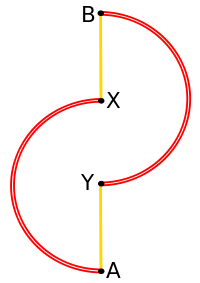
\includegraphics[width=0.35\textwidth]{img/braess1}
	\caption{Schemat przykładowego wyjściowego układu drogowego}
	\label{fig:wyjsciowy_uklad_drogowy}
\end{figure}

Poniżej znajduje się opis dostępnej sieci drogowej przedstawionej na rysunku~\ref{fig:wyjsciowy_uklad_drogowy}.

Autostrady to:\newline
AX, $t_{AX}(p) =  50 + p$ min\newline
YB, $t_{YB}(p) =  50 + p$ min\newline

Drogi lokalne to:\newline
AY, $t_{AY}(p) =  10p$ min\newline
XB, $t_{XB}(p) =  10p$ min\newline

Aut jest 6000 i~wszystkie mają za zadanie przejechać trasę z~$A$ do $B$.

\subsubsection{Analiza równowagi Nasha}
Każde auto musi zdecydować się na wybór trasy: albo $AXB$, albo $AYB$. \textbf{Równowaga Nasha} to taka sytuacja, w~której każdy z~samochodów spowoduje wydłużenie swojego czasu jazdy, zmieniając decyzję dotyczącą wyboru trasy przy niezmienionych decyzjach pozostałych aut. Jeśli $p$ i~$q$ oznaczają liczby aut w~tysiącach, pokonujących odpowiednio trasy $AXB$ i~$AYB$, to na podstawie danych do rysunku~\ref{fig:wyjsciowy_uklad_drogowy} otrzymuje się równania:

\begin{center}
\begin{math}\label{eq:nash1}
p+q = 6 \newline
t_{AX}(p)+t_{XB}(p) = t_{AY}(q) + t_{YB}(q) \newline
50+p+10p = 10q+50+q \newline
\end{math}
\end{center}

Rozwiązaniem równania jest $p=q=3$. Wynik może zostać wykorzystany do obliczenia średniego czasu przejazdu aut po dostępnej sieci drogowej. Przy tej gęstości ruchu pokonanie obu dostępnych tras zabiera $50+3+30=83$ minuty.

\subsection{Przykładowy uzupełniony układ drogowy}
Pamiętając o~początkowym stanie dróg i~średnim czasie przejazdu, układ drogowy zostaje uzupełniony o~autostradę, mającą na celu skrócenie czasu potrzebnego na podróż pomiędzy punktami w~grafie.

\subsubsection{Sieć drogowa i~auta}
Do wyjściowego układu drogowego dodana zostaje autostrada $YX$. Uzupełniony układ drogowy zaprezentowany jest na rysunku~\ref{fig:wyjsciowy_uklad_drogowy2}.

\begin{figure}[htbp]
	\centering
	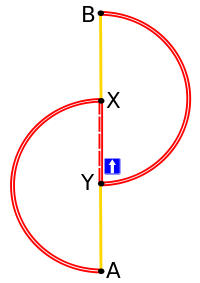
\includegraphics[width=0.35\textwidth]{img/braess2}
	\caption{Schemat przykładowego uzupełnionego układu drogowego}
	\label{fig:wyjsciowy_uklad_drogowy2}
\end{figure}

Poniżej znajduje się opis dotyczący uzupełnionego fragmentu sieci drogowej, przedstawionej na rysunku~\ref{fig:wyjsciowy_uklad_drogowy2}.

Autostrady to:\newline
YX, $t_{YX}(p) =  10 + p$ min\newline

Aut jest nadal 6000 i~wszystkie mają za zadanie przejechać trasę z~$A$ do $B$.

\subsubsection{Analiza równowagi Nasha}
Jeśli $p$, $q$ i~$r$ oznaczają liczby aut w~tysiącach pokonujących odpowiednio trasy $AXB$, $AYB$ i~$AYXB$, to na podstawie danych do rysunku~\ref{fig:wyjsciowy_uklad_drogowy2} otrzymuje się równania:

\begin{center}
\begin{math}
p+q+r = 6 \newline
t_{AX}(p)+t_{XB}(p+r) = t_{AY}(q+r) + t_{YB}(q) = t_{AY}(q+r)+t_{YX}(r)+t_{XB}(p+r)\newline
50+p+10(p+r) = 10(q+r)+50+q = 10(q+r)+ 10 + r + 10(p+r)\newline
\end{math}
\end{center}

Rozwiązaniem równania jest $p=q=r=2$. Wynik może zostać wykorzystany do obliczenia średniego czasu przejazdu aut po dostępnej sieci drogowej. Czas przejazdu dla każdej z~tych dróg wynosi wówczas $50+2+10 \cdot (2+2)=92$ minuty.

\subsection{Wyjaśnienie intuicyjne paradoksu Braessa}
Wąskim gardłem systemu są drogi lokalne, na których czas przejazdu bardzo szybko wzrasta wraz z~intensywnością ruchu. Po pojawieniu się dodatkowej drogi dostępna staje się nowa trasa, prowadząca oprócz nowego skrótu YX tylko drogami lokalnymi.

Z perspektywy całości systemu nowy odcinek drogowy odciąża ruch na autostradach, gdzie jest to mało odczuwalne, a~w~zamian jeszcze bardziej zagęszcza ruch na drogach lokalnych, powodując wydłużenie czasu podróży~\cite{conference}.

W 1983 roku Steinberg i~Zangwill przeprowadzili eksperyment, który miał na celu oszacować występowanie paradoksu Braessa. Zaskakujący wynik, dla losowo dodawanych łącz potwierdził skomplikowanie problemu. Przede wszystkim udowodnione zostało, że przy zastosowaniu odpowiednich założeń, dla dowolnej sieci transportowej możliwe jest wystąpienie paradoksu. Niestety, szacunkowo pojawienie się paradoksu Braessa jest czysto losowe~\cite{paradox-dowod}. Paradoks mimo wszystko został z~powodzeniem zastosowany w~wielu miastach na świecie:

\begin{itemize}
\item Korea Południowa, Seul. Zostało zaobserwowane przyśpieszenie ruchu w~mieście po usunięciu autostrady w~ramach projektu renowacji okolicy Cheonggyecheon.

\item Niemcy, Stuttgart. Zostały zlikwidowane drogi zbudowane w~latach 60-tych XX wieku.

\item USA, Nowy Jork. Czasowe zamknięcie ulicy 42 zniwelowało ilość zatorów w~okolicy.

\item W~2008 roku Youn, Gastner i~Jeong wykazali specyficzne drogi w~Bostonie, Nowym Jorku i~Londynie, których zamknięcie może zmniejszyć przewidywany czas podróży.

\item Kanada, Winnipeg.
\end{itemize}

\section{Klasyczny algorytm genetyczny}
Dla dużej klasy ważnych zadań nie opracowano dotąd dostatecznie szybkich algorytmów ich rozwiązywania. Dla takich zadań optymalizacji często można znaleźć wydajny algorytm, który nie gwarantuje jednak uzyskania rozwiązania optymalnego, a~tylko w~przybliżeniu optymalne. Dla niektórych trudnych zadań optymalizacji można używać algorytmów probabilistycznych jednak one również nie gwarantują, że zostanie uzyskane rozwiązanie optymalne.

Ogólnie, jakąkolwiek czynność do wykonania można przedstawić jako rozwiązywanie zadania co można z~kolei rozumieć jako przeszukiwanie przestrzeni możliwych rozwiązań.~Ponieważ zależy nam na ,,najlepszym'' rozwiązaniu, można uważać to zadanie za proces optymalizacji. W~małych przestrzeniach klasyczne metody pełnego przeszukiwania zwykle wystarczają. W~większych przestrzeniach trzeba niestety stosować specjalizowane metody sztucznej inteligencji. Wśród tych metod znajdują się algorytmy genetyczne~\cite{genetyczne-dane=ewo}.

\subsection{Podstawowe pojęcia algorytmów genetycznych}
Idea algorytmu genetycznego została zaczerpnięta z~nauk przyrodniczych, opisujących zjawiska doboru naturalnego i~dziedziczenia. Mechanizmy te polegają na przetrwaniu osobników najlepiej dostosowanych w~danym środowisku, podczas gdy osobniki gorzej przystosowane są eliminowane. Z~kolei te osobniki, które przetrwają, przekazują informację genetyczną swoim potomkom. Krzyżowanie informacji genetycznej otrzymanej od ,,rodziców'' prowadzi do sytuacji, w~której kolejne pokolenia są przeciętnie coraz lepiej dostosowane do warunków środowiska. Zachodzi tu więc swoisty proces optymalizacji~\cite{genetyczne}. 

\begin{definition}
\textbf{Populacją} nazywa się zbiór osobników o~określonej liczebności.
\end{definition}

\begin{definition}
\textbf{Osobnikami} populacji w~algorytmach genetycznych są zakodowane w~postaci chromosomów zbiory parametrów zadania, czyli rozwiązania, określone też jako punkty przestrzeni poszukiwań.~Osobniki czasami nazywa się organizmami.
\end{definition}

\begin{definition}
\textbf{Chromosomy}, inaczej łańcuchy lub ciągi kodowe, to uporządkowane ciągi genów.
\end{definition}

\begin{definition}
\textbf{Gen}, nazywany też cechą, znakiem, detektorem, stanowi pojedynczy element genotypu, w~szczególności chromosomu. Genotyp, czyli struktura, to zespół chromosomów danego osobnika. Zatem osobnikami populacji mogą być genotypy albo pojedyncze chromosomy.
\end{definition}

\begin{definition}
\textbf{Fenotyp} jest zestawem wartości, odpowiadających danemu genotypowi, czyli zdekodowaną strukturą, a~wiec jest zbiorem parametrów zadania (rozwiązaniem, punktem przestrzeni poszukiwań).
\end{definition}

\begin{definition}
\textbf{Allel} to wartość danego genu, określona jako wartość cechy lub wariant cechy.
\end{definition}

\begin{definition}
\textbf{Locus} to pozycja, która wskazuje miejsce położenia danego genu w~łańcuchu, czyli chromosomie.
\end{definition}

\begin{definition}
\textbf{Funkcja przystosowania} nazywana też \textbf{funkcją dopasowania lub funkcją oceny}. Stanowi ona miarę przystosowania (dopasowania) danego osobnika w~populacji.
\end{definition}

\subsection{Klasyczny algorytm genetyczny}
Na podstawowy (klasyczny) algorytm genetyczny, nazywany także elementarnym lub prostym, składają się następujące kroki:

\begin{enumerate}
\item inicjacja, czyli wybór początkowej populacji chromosomów,
\item ocena przystosowania chromosomów w~populacji,
\item sprawdzenie warunku zatrzymania,
\item selekcja chromosomów,
\item zastosowanie operatorów genetycznych,
\item utworzenie nowej populacji,
\item wyprowadzenie najlepszego chromosomu.
\end{enumerate}

Najłatwiej wyobrazić sobie powyższe kroki analizując je na schemacie przedstawionym na rysunku~\ref{fig:ogolny_schemat_alg_genetycznego}. Następnie omówiono wszystkie kroki algorytmu~\cite{gene}.

\begin{figure}[htbp]
	\centering
	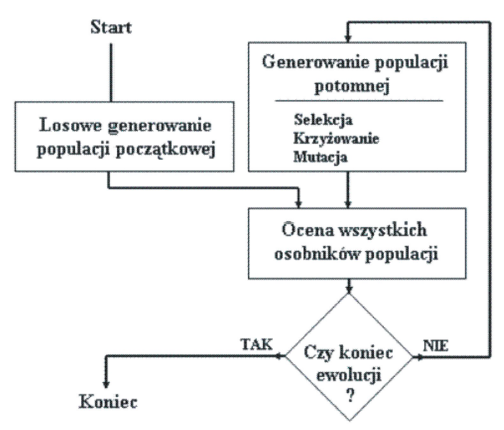
\includegraphics[width=0.6\textwidth]{img/ogolgene}
	\caption{Ogólny schemat algorytmu genetycznego}
	\label{fig:ogolny_schemat_alg_genetycznego}
\end{figure}

\textbf{Inicjacja, czyli utworzenie populacji początkowej}, polega na losowym wyborze żądanej liczby chromosomów (osobników) reprezentowanych przez ciągi binarne o~określonej długości. Ta metoda tworzenia populacji początkowej w~pewnych sytuacjach nie jest efektywna, gdyż wiele osobników może nie spełniać ograniczeń występujących w~rozwiązywanym zadaniu. W~takich przypadkach dobrze jest odwołać się do wiedzy o~rozwiązywanym problemie i~,,zaprojektować'' zestaw chromosomów.

\textbf{Ocena przystosowania chromosomów w~populacji} opiera się na obliczeniu wartości funkcji przystosowania dla każdego chromosomu z~tej populacji. Zwykle im większa jest wartość funkcji, tym lepsza ,,jakość'' chromosomów. Postać funkcji przystosowania zależy od rodzaju rozwiązywanego problemu. Zwykle zakłada się, że funkcja przystosowania przyjmuje zawsze wartości nieujemne, a~ponadto, że rozwiązywany problem optymalizacji jest problemem poszukiwania maksimum tej funkcji. Oczywiście, pierwotną postać funkcji przystosowania można łatwo sprowadzić do innej postaci.

\textbf{Sprawdzanie warunku zatrzymania}. Określenie warunku zatrzymania algorytmu genetycznego zależy od konkretnego zastosowania tego algorytmu. W~zagadnieniach optymalizacji, jeśli znana jest wartość oczekiwana funkcji przystosowania, zatrzymanie algorytmu może nastąpić po uzyskaniu tej wartości. Ewentualnie określana jest pewna dokładność porównania. Zatrzymanie algorytmu może również nastąpić, gdy jego dalsze działanie nie poprawia już uzyskanej najlepszej wartości. Zwykle jednak, algorytm jest zatrzymywany po upływie określonego czasu działania lub po określonej liczbie iteracji. Jeśli warunek zatrzymania jest spełniony, następuje przejście do ostatniego kroku, czyli wyprowadzenia ,,najlepszego'' chromosomu.

\textbf{Selekcja chromosomów} polega na wybraniu na podstawie obliczonych wartości funkcji przystosowania, tych chromosomów, które będą brały udział w~tworzeniu potomków do następnego pokolenia, czyli następnej generacji. Wybór ten zwykle odbywa się zgodnie z~zasadą naturalnej selekcji, to znaczy największe szanse na udział w~tworzeniu nowych osobników mają chromosomy o~największej wartości funkcji przystosowania. Istnieje wiele metod selekcji populacji.

\textbf{Zastosowanie operatorów genetycznych}. W~klasycznym algorytmie genetycznym stosuje się dwa podstawowe operatory genetyczne: operator
krzyżowania oraz operator mutacji. Należy jednak zaznaczyć, że operator
mutacji odgrywa zdecydowanie drugoplanową rolę w~stosunku do operatora krzyżowania. Oznacza to, ze krzyżowanie w~klasycznym algorytmie genetycznym występuje prawie zawsze, podczas gdy mutacja dość rzadko. 

\textit{Operacja krzyżowania} jest podstawową operacją algorytmów genetycznych, służącą do rekombinacji materiału genetycznego. Operacja opiera się na dwóch chromosomach, których części materiału genetycznego zostają wymieszane w~celu utworzenia nowego chromosomu. Podstawowa operacja krzyżowania opiera się na jednym punkcie krzyżowania i~została przedstawiona na poglądowym rysunku~\ref{fig:krzyzowanie_schemat}~\cite{genetyczne-dane=ewo}

\begin{figure}[htbp]
	\centering
	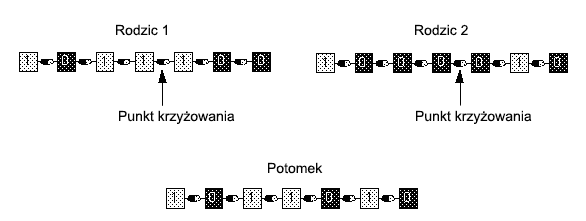
\includegraphics[width=\textwidth]{img/crossover}
	\caption{Ogólny schemat operacji krzyżowania osobników}
	\label{fig:krzyzowanie_schemat}
\end{figure}

Proces rekombinacji przez krzyżowanie nie byłby w~stanie odkryć całej przestrzeni poszukiwań, jeżeli dana kombinacja nie byłaby obecna w~sekcjach populacji. To mogłoby prowadzić do błędnego wyniku. \textit{Operacja mutacji} pozwala na wprowadzenie nowych struktur genetycznych w~obecnej populacji. Dokonuje się tego poprzez losową zmianę dowolnego genu w~chromosomie. Sytuacja jest przedstawiona na poglądowym rysunku~\ref{fig:mutacja_schemat}~\cite{genetyczne-dane=ewo}.

\begin{figure}[htbp]
	\centering
	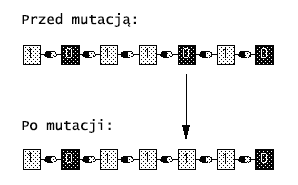
\includegraphics[width=0.580\textwidth]{img/mutation}
	\caption{Ogólny schemat operacji mutacji osobników}
	\label{fig:mutacja_schemat}
\end{figure}

\textbf{Utworzenie nowej populacji}. Chromosomy otrzymane w~wyniku działania operatorów genetycznych na chromosomach tymczasowej populacji rodzicielskiej wchodzą w~skład nowej populacji. Populacja ta staje się tak zwaną populacją bieżącą dla danej iteracji algorytmu genetycznego. W~każdej kolejnej iteracji oblicza się wartość funkcji przystosowania każdego z~chromosomów tej populacji. Następnie sprawdza się warunek zatrzymania algorytmu i~albo wyprowadza się wynik w~postaci chromosomu o~największej (najmniejszej) wartości funkcji przystosowania, albo przechodzi się do kolejnego kroku algorytmu genetycznego, to jest selekcji. W~klasycznym algorytmie genetycznym cała poprzednia populacja chromosomów zastępowana jest przez tak samo liczną nową populację potomków.

\textbf{Wyprowadzenie ,,najlepszego'' chromosomu}. Jeżeli spełniony jest warunek zatrzymania algorytmu genetycznego, należy wyprowadzić wynik algorytmu genetycznego, czyli podać rozwiązanie problemu. Najlepszym rozwiązaniem jest chromosom o~największej lub najmniejszej wartości funkcji przystosowania.

\subsection{Metody selekcji osobników}\label{sec:selekcja}
W algorytmach genetycznych wyróżnia się etap selekcji, który z~bieżącej populacji osobników wybiera te o~największej wartości funkcji przystosowania do populacji rodzicielskiej.

\textbf{Metoda ruletki (koła ruletki)} jest jedną z~najbardziej podstawowych metod selekcji. Polega na utworzeniu koła ruletki z~polami odpowiadającymi poszczególnym chromosomom. Wielkość pól jest proporcjonalna do wartości funkcji przystosowania. Proces selekcji oparty jest na obrocie ruletką tyle razy ile osobników jest w~populacji i~na wyborze za każdym razem jednego chromosomu do nowej populacji. Pewne chromosomy są wybierane więcej niż jeden raz, niektóre dokładnie raz, a~niektóre wcale~\cite{genetyczne-dane=ewo}. Jest to metoda prosta i~daje w~miarę zadowalające wyniki. Ma jednak wady. Jedną z~nich jest możliwość stosowania metody ruletki tylko do jednej klasy zadań, tzn. tylko do maksymalizacji (lub tylko do minimalizacji). Takie ograniczenie jest niewątpliwie jej wadą. Bardziej istotną wadą metody ruletki jest zbyt wczesne eliminowanie z~populacji osobników o~bardzo małej wartości funkcji przystosowania. Może to prowadzić do zbyt wczesnej zbieżności algorytmu. Metoda ta została zobrazowana na rysunku~\ref{fig:selekcja_ruletka}.

\begin{figure}[htbp]
	\centering
	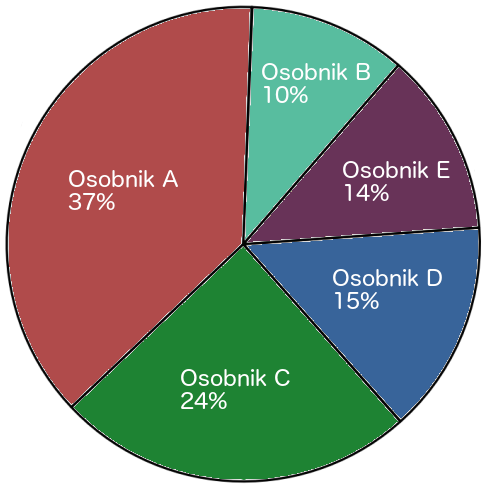
\includegraphics[width=0.35\textwidth]{img/selekcja_roul}
	\caption{Schemat selekcji osobników metodą koła ruletki} 
	\label{fig:selekcja_ruletka}
\end{figure}

\textbf{W selekcji rankingowej} osobniki populacji są ustawiane kolejno w~zależności od funkcji przystosowania to znaczy od najlepiej do najgorzej przystosowanego. Każdemu osobnikowi przyporządkowana jest liczba zwana
rangą i~oznaczająca jego pozycję na liście. Liczba kopii danego osobnika wprowadzonych do nowej populacji jest ustalana na podstawie wcześniej zdefiniowanej funkcji, zależnej od rangi.

\textbf{Selekcja turniejowa}, polega na podzieleniu populacji na podgrupy k-elementowe (k to rozmiar turnieju – zwykle $2$ lub $3$) i~wyborze z~każdej podgrupy osobnika o~najlepszym przystosowaniu. Można to zrobić poprzez wybór losowy lub wybór deterministyczny. Wtedy wyboru dokonuje się z~prawdopodobieństwem równym $1$. Taki mechanizm wyboru rodziców posiada szereg zalet. Po pierwsze, w~przypadku małych grup o~rozmiarze $k$ zapewnia to szanse przetrwania $k-2$ najlepszym osobnikom, co z~kolei gwarantuje, że dostosowanie populacji nie pogarsza się w~trakcie kolejnych iteracji. Po drugie, bez względu na to, jak dobrze dostosowany jest osobnik w~porównaniu z~reszta populacji, produkuje on co najwyżej jednego potomka w~każdej iteracji. Własność ta zapobiega przedwczesnej zbieżności populacji – problemowi, z~którym boryka się większość modeli ewolucji. W~selekcji proporcjonalnej osobnik o~wysokim dostosowaniu dominuje początkowe etapy ewolucji, co skutecznie ogranicza obszar poszukiwań i~powoduje zbieżność populacji do rozwiązań suboptymalnych. Po trzecie, metoda turniejowa nadaje się zarówno do problemów maksymalizacji, jak i~minimalizacji~\cite{genetyczne-immunologiczne}. 

W klasycznym algorytmie genetycznym możliwa jest sytuacja, w~której do nowej populacji nie zostaną wybrane najlepsze osobniki poprzedniej populacji. Chcąc zapobiec takiej sytuacji stosuje się \textbf{strategię elitarnej selekcji}. W~jej przypadku nacisk położony jest na zachowanie w~kolejnych iteracjach najlepiej przystosowanych osobników. Dzięki temu zachowywane jest najlepsze rozwiązanie (lub $N$ najlepszych rozwiązań) pomiędzy iteracjami~\cite{genetyczne-dane=ewo}. Strategia ta powoduje, że potomstwo elity będzie dominować przyszłe populacje. Może to ograniczać zdolności eksploracyjne algorytmu, gdyż początkowa elita niekoniecznie zawiera geny charakteryzujace najlepsze osobniki. Rozwiązaniem jest utrzymywanie elity o~niewielkim rozmiarze, podobnie jak ma to miejsce w~pojedynczej selekcji turniejowej, gdzie elita składa się z~dwóch osobników.

\subsection{Mocne i~słabe strony algorytmów genetycznych}
Początkowo algorytmy genetyczne były głównie założeniem teoretycznym. Dziś są szeroko wykorzystywanymi rozwiązaniami do wielu problemów badawczych jak również są stosowane w~przypadku zastosowań komercyjnych. Oczywiście jedną z~przyczyn, której algorytmy genetyczne zawdzięczają swój sukces jest rosnąca moc obliczeniowa komputerów oraz rozwój Internetu. Są one wykorzystywane w~wielu bardzo różnych dziedzinach jak badania rynku akcji i~prognozy portfela, planowanie, projektowanie inżynierii kosmicznej i~mikroprocesorowej, biochemii i~biologii molekularnej oraz planowania tras w~portach lotniczych i~liniach montażowych. Potencjał algorytmów ewolucyjnych nie jest z~pewnością jeszcze w~pełni wykorzystany.

To wszystko jest możliwe dzięki wielu mocnym stronom algorytmów genetycznych:
\begin{itemize}
\item Mogą rozwiązać każdy problem optymalizacji, który może być opisane za pomocą kodowania chromosomów.
\item Rozwiązują problemy posiadające wiele rozwiązań.
\item Budowa algorytmów genetycznych nie ma związku z~rozwiązywanym problemem, dzięki czemu mogą rozwiązywać problemy wielowymiarowe, nieróżniczkowalne, nieciągłe, a~nawet nieparametryczne.
\item Są bardzo łatwe do zrozumienia i~praktycznie nie wymagają znajomości matematyki.
\item Są łatwo adoptowane do istniejących symulacji i~modeli.
\end{itemize}

Oczywiście, istnieją też wady tych rozwiązań:
\begin{itemize}
\item Pewne problemy optymalizacji, nie mogą być rozwiązane za pomocą algorytmów genetycznych. Dzieje się tak, gdy nie jest możliwe określenie prawidłowej funkcji przystosowania chromosomu, co zaburza system ewolucji najlepszych rozwiązań.
\item Nie ma pewności, że algorytm genetyczny znajdzie optymalne rozwiązanie.
\item Podobnie jak w~przypadku innych metod sztucznej inteligencji, nie możliwe jest przewidzenie czasu działania optymalizacji przy pomocy algorytmu genetycznego.
\item Algorytm genetyczny czasu rzeczywistego są zawodne z~powodu przypadkowych rozwiązań i~konwergencji. Oznacza to, że podczas gdy populacja zawsze zmierza do lepszego wyniku, nie dotyczy to pojedynczego osobnika.
\end{itemize}

\section{Teoria grafów}
Wiele sytuacji z~życia codziennego może zostać wygodnie opisanych za pomocą diagramów składających się z~zestawu punktów oraz linii łączących określone pary tych punktów. Punkty mogą reprezentować ludzi a~połączenia znajomości lub może to być odzwierciedlenie ośrodków komunikacyjnych oraz ich połączeń.~Warto zauważyć, że w~dziedzinie tych problemów nie jest interesującym sposób połączenia ani typ punktów a~jedynie abstrakcyjnie matematyczny koncept takiej sytuacji~\cite{teoria-grafow-z-zast}.

\subsection{Geneza teorii grafów}
Zagadnienie mostów królewieckich jest historycznym problemem matematycznym. Rozwiązanie zaproponowane w~1735 roku przez szwajcarskiego matematyka i~fizyka Leonharda Eulera dało początek teorii grafów. Królewiec leżący w~Królestwie Prus (dzisiaj Kaliningrad, Rosja), znajduje się nad brzegiem rzeki Pregoła. Miasto posiada dwie duże wyspy, które połączone są ze sobą siedmioma mostami. Historyczna mapa przedstawiona na rysunku~\ref{fig:mapa_krolewiec} świetnie ilustruje tę sytuację~\cite{teoria-grafow}.

\begin{figure}[htbp]
	\centering
	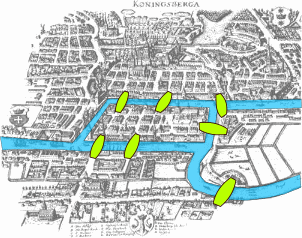
\includegraphics[width=0.50\textwidth]{img/konigsberg_bridges}
	\caption{Mapa królewieckich mostów z czasów Eulera} 
	\label{fig:mapa_krolewiec}
\end{figure}

Problemem postawionym matematykowi było znalezienie takiej drogi, która przekroczy każdy most raz i~tylko raz. Wyspa nie była dostępna ze strony miasta w~żaden inny sposób niż przez most. Dodatkowo przekroczenie każdego mostu musiało odbyć się w~pełni, to znaczy nie dozwolonym było zawracanie na środku mostu. Pierwszą obserwacją Eulera był fakt, że dokładna pozycja w~mieście nie jest istotna. To pozwoliło mu na uproszczenie problemu do abstrakcyjnej formy, dając początki teorii grafów (Rys.~\ref{fig:krolewiec_simple}).

\begin{figure}[htbp]
	\centering
	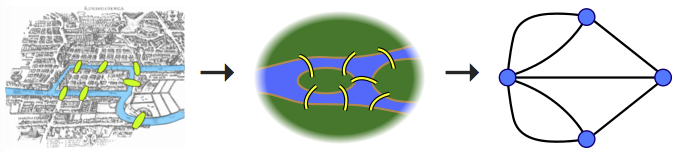
\includegraphics[width=0.90\textwidth]{img/bridge_uproszczenie}
	\caption{Schemat przekształcenia problemu mostów królewieckich w graf} 
	\label{fig:krolewiec_simple}
\end{figure}

Matematyk dowiódł, że nie jest możliwe rozwiązanie tego problemu. W~efekcie stworzył jednak definicję która jasno określa warunki, które muszą być spełnione by taka sytuacja mogła mieć miejsce. Rozważał on też podobny problem, w~którym zakończenie drogi jest tym samym punktem co jej początek. Obie definicje do dziś nazywa się nazwiskiem odkrywcy.

\begin{definition}
\textbf{Ścieżka Eulera} \textit{(ang. Eulerian path)} jest ścieżką w~grafie, która przechodzi dokładnie jeden raz przez każdą jego krawędź. Aby taka ścieżka istniała, graf musi być spójny oraz każdy jego wierzchołek za wyjątkiem dwóch musi posiadać parzysty stopień.
\end{definition}

\begin{definition}
\textbf{Cykl Eulera} \textit{(ang. Eulerian cycle)} jest ścieżką w~grafie, która przechodzi przez wszystkie jego krawędzie i~kończy się w~wierzchołku startowym. Aby istniał cykl Eulera, graf musi być spójny oraz każdy jego wierzchołek musi posiadać stopień parzysty.
\end{definition}

Opis zagadnienia opublikowany przez Eulera w~pracy \textit{Solutio problematis ad geometriam situs pertinentis} w~\textit{Commentarii academiae scientiarum Petropolitanae} jest uznawany za pierwszą pracę na temat teorii grafów.

\subsection{Podstawowe pojęcia dotyczące grafów}\label{sec:podstawy_grafy}

\begin{definition}\label{def:graf_nieskierowany}
\textbf{Grafem (nieskierowanym)} nazywa się parę zbiorów $(V,E)$. Elementy zbioru $V$ nazywają się \textit{wierzchołkami}, natomiast elementy zbioru $E$ to \textit{krawędzie}. Każda krawędź jest parą wierzchołków, tzn. $E \subseteq {{u,v}:u,v \in V}$~\cite{grafy}.
\end{definition}

\begin{figure}[htbp]
	\centering
	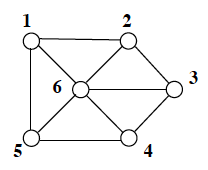
\includegraphics[width=0.40\textwidth]{img/graf1}
	\caption{Przykładowy graf nieskierowany} 
	\label{fig:graf_nieskierowany}
\end{figure}

Przykładowy graf nieskierowany (Rys.~\ref{fig:graf_nieskierowany}) może zostać opisany przez zbiory:
$
V=\{1,2,3,4,5,6\}, 
E=\{\{1,2\},\{1,5\},\{2,3\},\{3,4\},\{4,5\},\{6,5\},\{6,1\},\{2,6\},\{3,6\},\{4,6\}\}
$

\begin{definition}
\textbf{Rząd grafu} (\textbf{ang. graph order}) to liczba wierzchołków w~grafie.
\end{definition}

\begin{definition}
\textbf{Rozmiar grafu} (\textbf{ang. graph size}) to liczba krawędzi w~grafie.
\end{definition}

Wierzchołki grafu przechowują informację, natomiast krawędzie określają sposób poruszania się po grafie: z~wierzchołka $u$ można przejść do wierzchołka $v$ tylko wtedy, gdy istnieje ścieżka (ciąg krawędzi), która prowadzi w~grafie od wierzchołka $u$ do $v$.

\begin{definition}
\textbf{Grafem zerowym} (\textbf{ang. null graph}) jest graf, który posiada wierzchołki, lecz nie posiada żadnych krawędzi.
\end{definition}

\begin{definition}
Wierzchołek nie połączony krawędzią z~żadnym innym wierzchołkiem grafu nazywa się \textbf{wierzchołkiem izolowanym} (\textbf{ang. isolated vertex}).
\end{definition}

\begin{definition}
Dane dwa wierzchołki mogą być połączone ze sobą za pomocą więcej niż jednej krawędzi, które nazywa się \textbf{krawędzią wielokrotną} (\textbf{ang. multi-edge}).
\end{definition}

\begin{definition}
Wierzchołek może łączyć się krawędzią z~samym sobą. Otrzymuje się wtedy tzw. \textbf{pętlę} (\textbf{ang. loop}). 
\end{definition}

\begin{definition}
Graf zawierający pętle lub krawędzie wielokrotne nazywa się \textbf{multigrafem} (\textbf{ang. multigraph}).
\end{definition}

\begin{definition}
Graf nie posiadający pętli oraz krawędzi podwójnych nazywa się \textbf{grafem prostym} (\textbf{ang. simple graph} lub \textbf{strict graph}).
\end{definition}

\begin{definition}
\textbf{Stopniem wierzchołka} (\textbf{ang. degree}) nazywa się liczbę krawędzi, które łączą się z~danym wierzchołkiem. Jeśli graf posiada pętle, to liczy się je za 2.
\end{definition}

\begin{definition}\label{def:graf_skierowany}
\textbf{Grafem skierowanym} nazywa się taki graf, w~którym każda krawędź ma zdefiniowany początek i~koniec, tzn. pary grafu muszą być uporządkowane. Wtedy $E \subseteq V \times V = {{u,v}:u,v \in V}$.
Krawędź $(u,v)$ najłatwiej wyobrazić sobie jako strzałkę od $u$ do $v$, dlatego często oznacza się ją przez $u \rightarrow v$~\cite{grafy}.
\end{definition}

\begin{figure}[htbp]
\centering
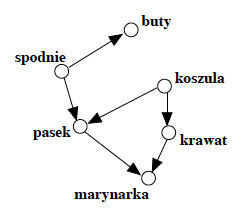
\includegraphics[width=0.40\textwidth]{img/graf2}
\caption{Przykładowy graf skierowany} 
\label{fig:graf_skierowany} 
\end{figure}

Przykładowy graf skierowany (Rys.~\ref{fig:graf_skierowany}) może zostać opisany przez zbiory:
\newline
\begin{math}
V=\{spodnie, buty, pasek, koszula, krawat, marynarka\}
\end{math}
\newline
\begin{math}
E=\{\{spodnie \rightarrow buty\},\{spodnie  \rightarrow pasek\},
	\{koszula \rightarrow pasek\},\{koszula \rightarrow krawat\},
	\{pasek \rightarrow marynarka\},\{krawat \rightarrow marynarka\}\}
\end{math}

\begin{definition}
\textbf{Ścieżka lub droga} (\textbf{ang. path}) jest uporządkowanym ciągiem kolejnych krawędzi, po których należy przejść, aby dotrzeć z~wierzchołka startowego (\textit{ang. start vertex}) do wierzchołka końcowego (\textit{ang. end vertex}). W~grafie może istnieć wiele różnych ścieżek pomiędzy dwoma wybranymi wierzchołkami.
\end{definition}

\begin{definition}
\textbf{Najkrótsza ścieżka} (\textbf{ang. shortest path}) to ta, która zawiera najmniej krawędzi/wierzchołków. Długość ścieżki (\textit{ang. path length}) to liczba zawartych w~niej krawędzi/wierzchołków.
\end{definition}

\begin{definition}
Mówi się, że \textbf{ścieżka jest prosta} (\textbf{ang. straight path} lub \textbf{simple path}), jeśli każdą krawędź/wierzchołek przechodzi się tylko jeden raz.
\end{definition}

\begin{definition}
\textbf{Cykl} (\textbf{ang. cycle}) to ścieżka, która rozpoczyna się i~kończy w~tym samym wierzchołku. Uwaga, nie mylić cyklu z~pętlą – pętla to pojedyncza krawędź.
\end{definition}

\begin{definition}
Graf nazywa się \textbf{acyklicznym} (\textbf{ang. acyclic graph}), jeśli nie posiada żadnych cykli.
\end{definition}

\subsection{Przeszukiwanie grafów}\label{sec:przeszukiwanie_grafow}
Przejście grafu \textit{(ang. graph traversal)} polega na przechodzeniu przez wierzchołki, do których prowadzą ścieżki. Algorytm przejścia daje nam pewność, że żaden taki wierzchołek nie zostanie pominięty.

\subsubsection{Przechodzenie grafów w~głąb – DFS}
Przeszukiwanie w~głąb \textit{(ang. Depth-First Search, DFS)} jest algorytmem o~prostej do zrozumienia idei. Na początku wszystkie wierzchołki grafu oznacza się jako nieodwiedzone, a~w~momencie dojścia do danego węzła grafu staje się on odwiedzony. Otóż rozpoczynając przechodzenie od wybranego, startowego wierzchołka grafu, porusza się się ,,w~głąb'' grafu poprzez wybieranie kolejnych krawędzi składających się na możliwie najprostszą ścieżkę aż do momentu, gdy nie można przejść do kolejnego, nieodwiedzonego jeszcze wierzchołka. Wówczas należy wrócić do węzła ostatnio odwiedzonego i~sprawdzić kolejną drogę (za pomocą krawędzi wychodzących z~niego do nieodwiedzonych węzłów). Czynność tę powtarza się rekurencyjnie dopóty, dopóki wszystkie wierzchołki, do których istnieje ścieżka z~węzła startowego, nie zostaną odwiedzone. W~przypadku, gdy w~grafie będą jeszcze nieodwiedzone wierzchołki, wówczas obiera się jeden z~nich jako nowy węzeł startowy i~ponownie rozpoczyna się przeszukiwanie. Metoda jest kontynuowana do momentu odwiedzenia wszystkich wierzchołków grafu. Metoda DFS jest zatem dobrym przykładem algorytmu z~powrotami. Przykładowe przejście grafu z~wykorzystaniem powyższej metody zostało zobrazowane na obrazku~\ref{fig:dfs}. Numery przy węzłach odpowiadają kolejności, w~której zostały odwiedzone.

\begin{figure}[htbp]
	\centering
	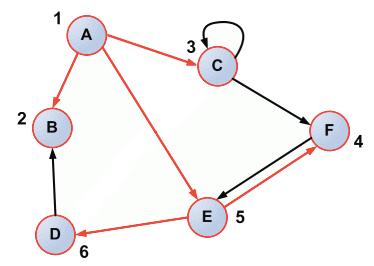
\includegraphics[width=0.45\textwidth]{img/dfs}
	\caption{Przykładowy graf z oznaczeniem kolejności odwiedzonych węzłów przy przeszukaniu metodą DFS}
	\label{fig:dfs}
\end{figure}

\subsubsection{Przechodzenie grafów wszerz – BFS}
Przeszukiwanie wszerz \textit{(ang. Breadth-First Search, BFS)} jest drugim z~najbardziej znanych sposobów przeszukiwania grafu. Zasada jest odmienna niż w~przypadku metody DFS – w~pierwszej kolejności przeglądany jest węzeł początkowy (źródłowy), następnie odwiedzane są po kolei węzły sąsiadujące ze źródłem, później wierzchołki sąsiednie (te jeszcze nieodwiedzone) sąsiadów źródła itd. A~zatem, jeśli wykorzystuje się listy sąsiedztwa do reprezentacji grafu, to najpierw przegląda się wierzchołki z~listy sąsiedztwa węzła początkowego, a~potem wierzchołki z~list sąsiedztwa węzłów, które znajdują się na liście przynależnej do źródła. W~skrócie można powiedzieć, że w~pierwszej kolejności algorytm dociera do węzłów oddalonych od wierzchołka początkowego o~jedną krawędź, potem o~dwie krawędzie itd. – stąd właśnie nazwa algorytmu, gdyż porusza się ,,wszerz'' na każdym kolejnym poziomie. Przykładowe przejście grafu z~wykorzystaniem powyższej metody zostało zobrazowane na obrazku~\ref{fig:bfs}. Numery przy węzłach odpowiadają kolejności, w~której zostały odwiedzone.

\begin{figure}[htbp]
	\centering
	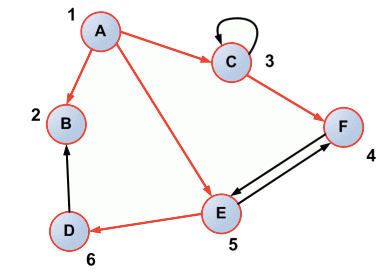
\includegraphics[width=0.45\textwidth]{img/bfs}
	\caption{Przykładowy graf z oznaczeniem kolejności odwiedzonych węzłów przy przeszukaniu metodą BFS}
	\label{fig:bfs}
\end{figure}

\subsection{Graf skierowany silnie spójny}\label{sec:graf_spojny}

\begin{definition}
\textbf{Grafem skierowanym silnie spójnym} nazywa się graf skierowany, w~którym możliwe jest dotarcie do każdego wierzchołka, zaczynając z~dowolnego innego poprzez dowolną ilość krawędzi. Wszystkie wierzchołki w~grafie skierowanym silnie spójnym muszą zatem posiadać przynajmniej jedną krawędź wchodzącą i~jedną wychodzącą~\cite{silniespojny}.
\end{definition}

\begin{definition}
\textbf{Składowa silnie spójna} (ang. strongly connected component) jest maksymalnym podgrafem, w~którym istnieją ścieżki pomiędzy każdymi dwoma wierzchołkami. Jeśli podgraf ten obejmuje wszystkie wierzchołki grafu, to mówi się, że dany graf skierowany jest silnie spójny (ang. strongly connected digraph). W~grafach nieskierowanych każdy graf spójny jest również silnie spójny. Poglądowo sytuacja ta jest przedstawiona na rysunku~\ref{fig:ex_silnie_spojna}.
\end{definition}

\begin{figure}[htbp]
	\centering
	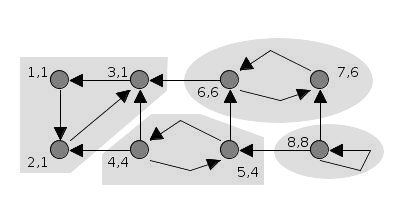
\includegraphics[width=0.7\textwidth]{img/tajran}
	\caption{Przykładowy graf z zaznaczonymi składowymi silnie spójnymi}
	\label{fig:ex_silnie_spojna}
\end{figure}

\subsubsection{Algorytm Kosaraju}
Najprostszą metodą poszukiwania składowych silnie spójnych w~grafie jest \textbf{algorytm Kosaraju}. Metoda ta korzysta z~reguły, że jeżeli wszystkie krawędzie grafu zostałyby odwrócone, składowe silnie spójne takiego grafu pozostają takie same jak w~przypadku grafu wejściowego. Wykorzystując tę wiedzę, algorytm wykonuje przejście wgłąb by znaleźć kolejność występowania wierzchołków. Następnie dokonywane jest ponowne przejście wgłąb, ale w~odwrotnej kolejności, bazując na porządku ustalonym podczas poprzedniego przejścia. Wykorzystując wcześniej wspomnianą regułę, tworząc ,,odwrócony'' graf, zaczynając od ostatniego wierzchołka pierwszego przejścia, wszystkie wierzchołki z~którymi jest on połączony tworzą składową silnie spójną. Ostatni krok powtarza się, aż do momentu gdy wszystkie wierzchołki zostaną sprawdzone.

\subsubsection{Algorytm Tarjana}
Algorytm ten w~porównaniu do poprzednika jest dwukrotnie szybszy ponieważ wykorzystuje jedynie jedno przejście wgłąb. Podstawowym założeniem\textbf{algorytmu  Tarjana}~\cite{tarjan} jest przeszukiwanie grafu w~głąb zaczynając od dowolnego wierzchołka wybranego w~sposób arbitralny. Tak, jak w~przypadku klasycznego przeszukiwania w~głąb, każdy sąsiadujący wierzchołek po odwiedzeniu zostaje oznaczony i~algorytm nigdy ponownie go nie odwiedza. Dzięki temu tworzy się kolekcję przeszukanych drzew, która jest drzewem rozpinającym grafu. Składowe silnie spójne są następnie odnajdowane jako poddrzewa, a~korzenie tych poddrzew są nazywane korzeniami składowych silnie spójnych. Każdy wierzchołek grafu może być wybrany na korzeń składowej silnie spójnej, jeśli zostanie wybrany jako pierwszy wierzchołek podczas przeszukiwania w~głąb.



\section{Sieć drogowa w~postaci grafu}
W przypadku sieci drogowej mowa oczywiście o~abstrakcyjnej strukturze sieci~\cite{reducingtheeffects}. Przez sieć drogową rozumie się bowiem układ dróg lub ulic na przykład w~mieście.W ramach pracy wykorzystano pewien fragment większej sieci. Przykładowo, było to miasto Sioux Falls w~Południowej Dakocie, prezentowane na rysunku~\ref{fig:fragment_sieci_siouxfalls}.

\begin{figure}[htbp]
	\centering
	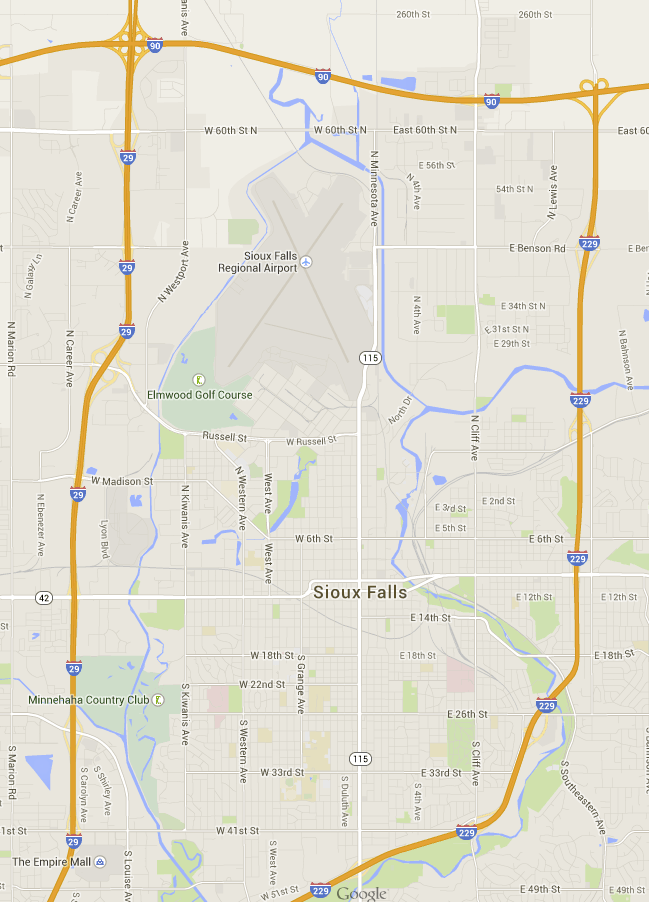
\includegraphics[width=0.42\textwidth]{img/siec}
	\caption{Fragment sieci drogowej miasta Sioux Falls, Południowa Dakota} 
	\label{fig:fragment_sieci_siouxfalls}
\end{figure}

Posługując się powyższą definicją grafu skierowanego, tworząc graf z~pewnej sieci drogowej, przyjmuje się, że zbiorem $V$ wierzchołków są skrzyżowania, natomiast zbiór krawędzi $E$ odnosi się do ulic pomiędzy tymi skrzyżowaniami. W~pracy posługiwano się zawsze grafem skierowanym. W~związku z~tym, w~przypadku ulic dwukierunkowych tworzone są pary krawędzi z~odpowiednimi kierunkami, nawet jeśli ulice nie są rozłączne w~rzeczywistości. Efekt transformacji fragmentu sieci drogowej zaprezentowanej w~postaci grafu skierowanego zaprezentowano na rysunku~\ref{fig:siouxfalls_ex_graf}.

\begin{figure}[htbp]
	\centering
	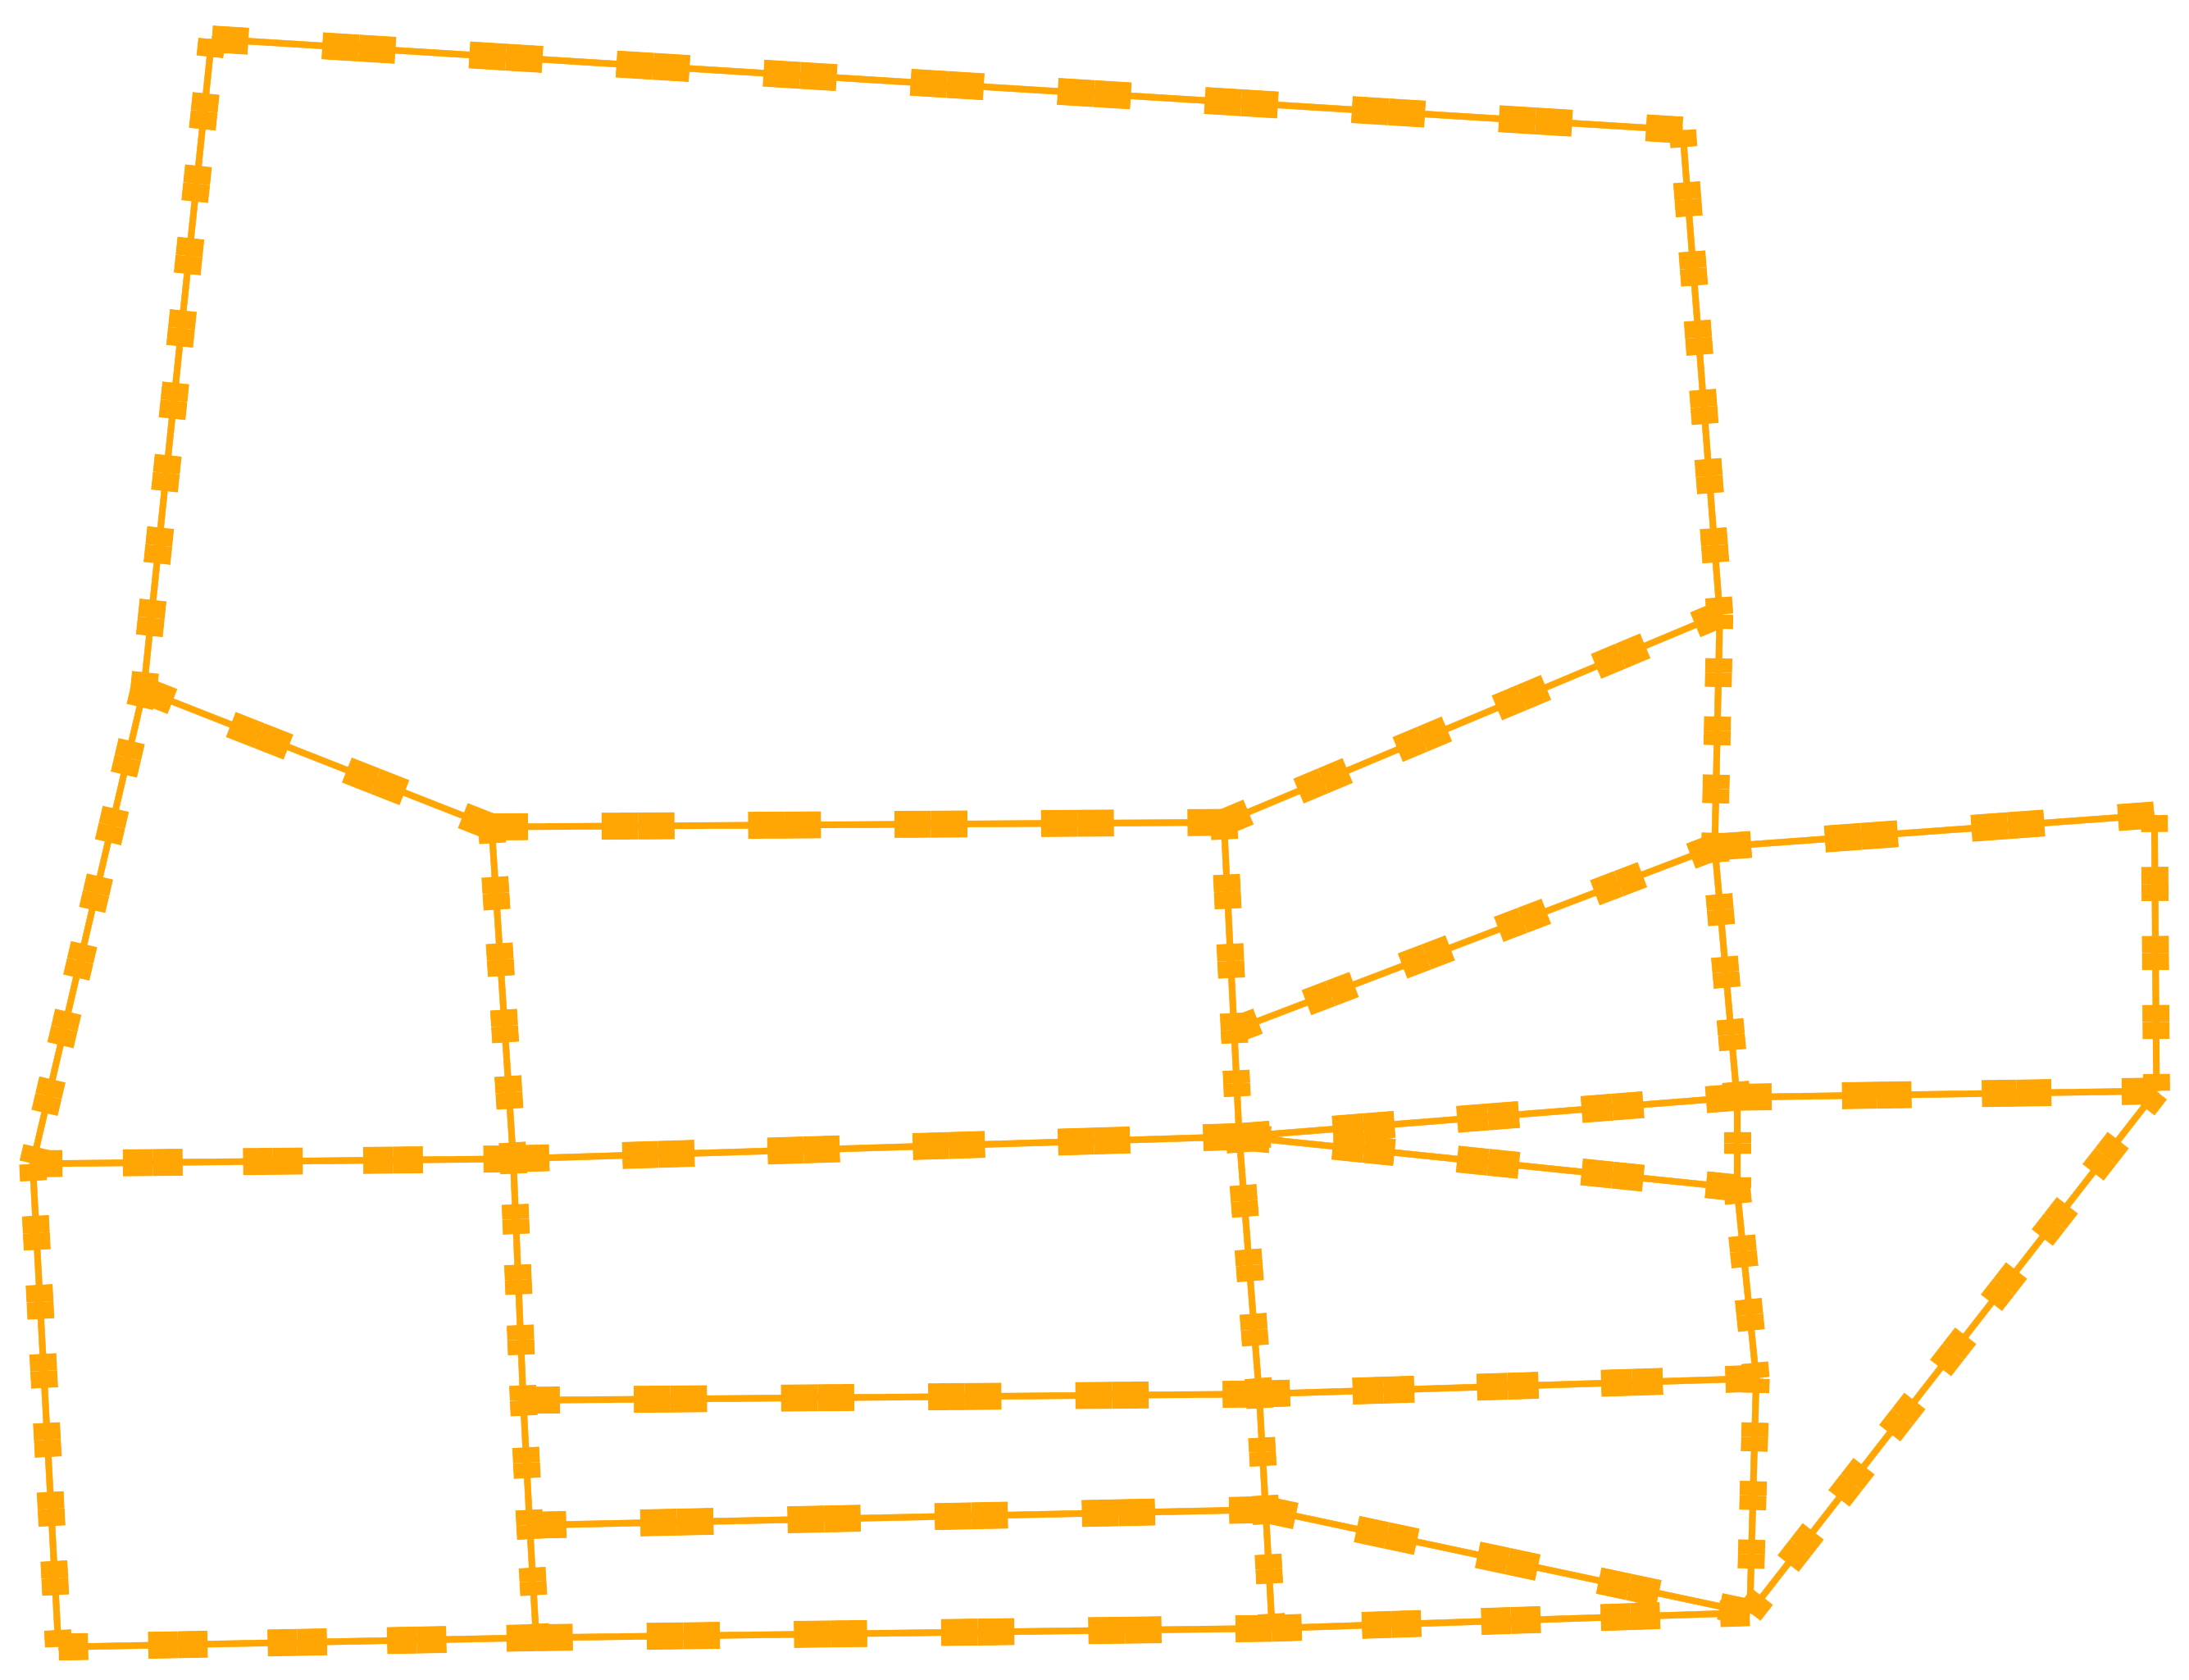
\includegraphics[width=0.5\linewidth]{img/graf}
	\caption{Sieć drogowa miasta Sioux Falls w postaci grafu}
	\label{fig:siouxfalls_ex_graf}
\end{figure}

Na pierwszy rzut oka nie jest widoczne podobieństwo pomiędzy mapą a~jej odzwierciedleniem w~postaci grafu. Wynika to z~braku dopasowania geometrycznego po przekształceniu. Na rysunku~\ref{fig:siouxfalls_ex_graf_geometry} prezentowana jest sieć drogowa miasta w~postaci grafu, po przekształceniu geometrycznym, tak by odzwierciedlał on mniej więcej ulice widoczne na mapie.

\begin{figure}[htbp]
	\centering
	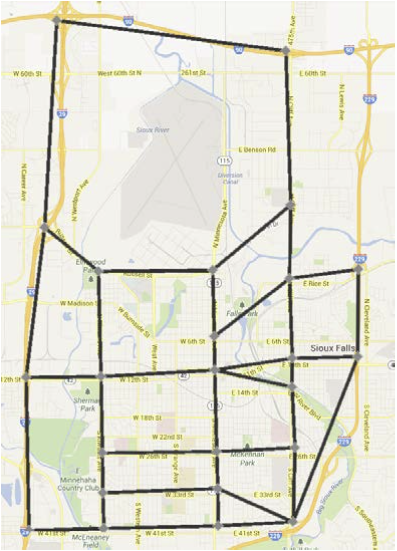
\includegraphics[width=0.42\linewidth]{img/dopasowanie}
	\caption{Graf sieci drogowej miasta z dopasowaną geometrią}
	\label{fig:siouxfalls_ex_graf_geometry}
\end{figure}

\section{Przystosowanie struktury grafu do użycia w~algorytmie genetycznym}

Niniejsza praca skupia się na optymalizacji grafów. W~tym wypadku klasyczna odmiana algorytmu genetycznego musiałaby zostać zmodyfikowana na potrzeby przedstawienia grafów jako chromosomów. Dodatkowo, wymagałoby to zastosowania nowych sposobów krzyżowania i~mutacji jednostek. 

Zdecydowano, że zamiast przystosowywać algorytm genetyczny do nowej struktury, struktura zostanie przystosowana do algorytmu. Ponieważ postawionym zadaniem jest zdecydowanie o~zamknięciu lub nie danej ulicy (krawędzi grafu), postanowiono przedstawić tę strukturę jako listę opisującą taki stan. Zgodnie z~tą myślą, sieć drogowa (graf) jest tłumaczona na listę elementów przyjmujących wartości:

\begin{itemize}
\item 1 (prawda) --- dla ulicy (węzła), który jest przejezdny,
\item 0 (fałsz) --- dla ulicy (węzła) zamkniętego dla ruchu.
\end{itemize}

Tworzona w~ten sposób lista stanów jest tak naprawdę tablicą booleanowską. Bez problemu może być zatem modyfikowana przez klasyczny algorytm genetyczny. Bardzo łatwym jest również odtworzenie obecnego stanu sieci drogowej. Przykładową sytuację przedstawiają rysunki~\ref{fig:bool_network_example} i~\ref{fig:graph_network_example}.

\begin{figure}[htbp]
	\centering
	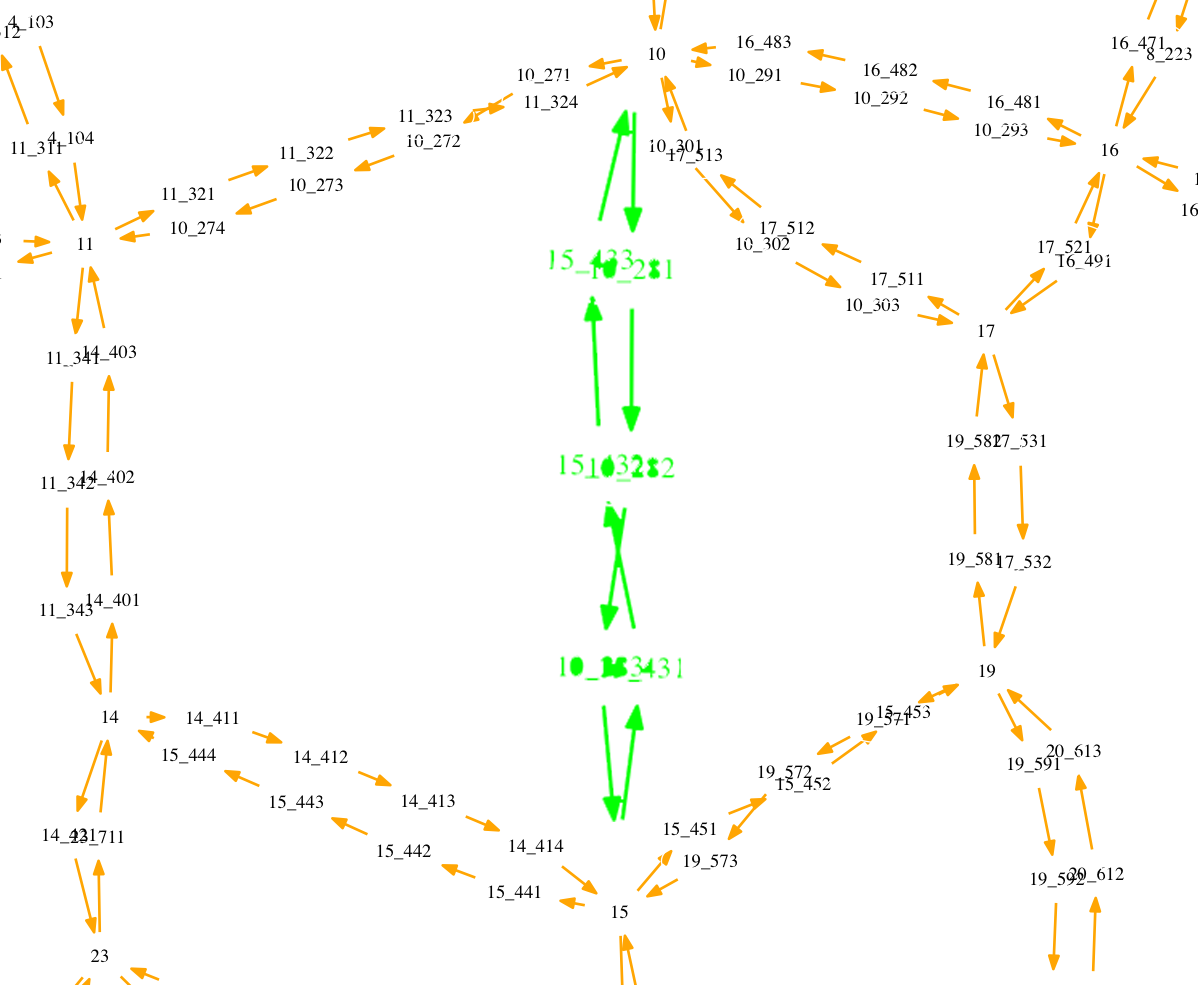
\includegraphics[width=0.5\textwidth]{img/bool-efect}
	\caption{Fragment sieci drogowej w postaci grafu}
	\label{fig:graph_network_example}
\end{figure}
\begin{figure}[htbp]
	\centering
	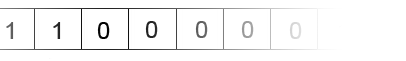
\includegraphics[width=0.5\textwidth]{img/bool}
	\caption{Fragment sieci drogowej w postaci tablicy binarnej }
	\label{fig:bool_network_example}
\end{figure}

Przedstawiony na rysunku~\ref{fig:bool_network_example} fragment sieci zawiera kolejne elementy zerowe, które w~tłumaczeniu na przykładowy graf są zaznaczone kolorem zielonym (Rys. \ref{fig:graph_network_example}). W~tym przypadku krawędzie te zostaną wyłączone z~ruchu.

W powyższym rozdziale zostały przybliżone matematyczne prawa i~twierdzenia użyte podczas realizacji pracy dyplomowej. Wyjaśniony został paradoks Braessa, który jest kluczowym założeniem pracy. Zaprezentowano struktury i~prawa użyte w~części praktycznej projektu GRoNO. W~kolejnym rozdziale znajduje się opis wybranego systemu symulacji wraz z~przedstawieniem miasta użytego w~badaniach.

\chapter{Metoda oceny struktury sieci drogowej}\label{rozdz.technologie} 
W niniejszym rozdziale opisana zostaje metoda oceny sieci drogowej modyfikowanej w~pracy. Opisano dokładnie wykorzystany w~tym celu system symulacji transportu ruchu drogowego wraz z~wykorzystanymi ustawieniami. Następnie przedstawiono przykładowe badane miasto, które zostało wykorzystane podczas badań wykonanych w~części praktycznej niniejszej pracy dyplomowej.

\section{Symulator transportu ruchu drogowego}
\textbf{MATSim} jest środowiskiem do implementacji szerokiej skali symulacji transportu, opartych na agentach. Składa się z~wielu modułów, które mogą zostać połączone lub używane oddzielnie. Moduły można zastępować własnymi implementacjami w~celu przetestowania pojedynczych aspektów pracy~\cite{matsim}. Obecnie \textit{MATSim} umożliwia modelowanie ruchu drogowego na podstawie symulacji transportu opartej na agentach. Odbywa się ono poprzez dostarczony kontroler, który w~sposób iteracyjny uruchamia symulacje oraz analizuje wyniki uzyskane poprzez wszystkie moduły systemu symulacji.

Możliwe jest wykorzystanie podstawowego zestawu funkcji \textit{MATSim} bez ingerencji w~środowisko. Odbywa się ono poprzez dostarczenie swoich danych wejściowych oraz dostosowanie konfiguracji symulacji. Dla bardziej zaawansowanych zastosowań może się jednak okazać konieczne dostarczenie własnych implementacji.

Głównymi cechami, którymi szczyci się symulator \textit{MATSim} są:
\begin{itemize}
\item \textbf{Symulacja zachowań mobilnych oparta na agentach.} Pokrycie odwzorowanych aktywności dotyczy jednego pełnego dnia, podczas którego (zwykle) duża liczba jednostek, agentów symulacji, jednocześnie bierze udział w~symulowanym scenariuszu. Możliwe jest odtworzenie zachowań zarówno prywatnego samochodu jak i~transportu publicznego w~bardzo dużej szczegółowości. Pozwala to na śledzenie każdego uczestnika symulacji (agenta) osobno, poprzez cały ich dzień - od wyjścia z~domu do pracy, poprzez wszystkie jego poboczne działania, aż do momentu powrotu.

\item \textbf{Szybkość i~stabilność działania.} \textit{MATSim} został przystosowany do obsługi nawet bardzo dużych scenariuszy symulacji transportu składających się z~milionów biorących w~niej udział agentów oraz setek tysięcy odcinków dróg.

\item \textbf{Analiza dostarczanych wyników.} Podczas symulacji transportu przechowywane są kluczowe wartości pozwalające szybko ocenić obecny stan tego procesu. Możliwe jest porównywanie wartości uzyskanych przez symulator z~rzeczywistymi danymi. Oprócz tego, \textit{MATSim} dostarcza szczegółowy opis przeprowadzonej symulacji, który może zostać łatwo przetworzony przez zewnętrzne aplikacje w~celu stworzenia autorskiej, szczegółowej analizy.

\item \textbf{Podejście modułowe.} Pozwala na łatwą wymianę lub dodawanie potrzebnych funkcjonalności. Umożliwia zastosowanie własnych algorytmów zachowań agentów symulacji lub stworzenie nowatorskiego silnika symulacji przy wykorzystaniu istniejących rozwiązań \textit{MATSim} dotyczących planowania tras.

\item \textbf{Stworzenie rozwiązanie w~ramach licencji otwartego oprogramowania.} Platforma jest rozpowszechniana na licencji \textit{GNU Public License (GPL)}. Oznacza to, że korzystanie z~\textit{MATSim} jest zupełnie darmowe. Ponadto, twórcy dostarczają kompletny kod źródłowy, który można modyfikować. Projekt \textit{MATSim} został stworzony w~oparciu o~język programowania \textit{Java} co pozwala na jego wykorzystanie we wszystkich głównych systemach operacyjnych w~tym \textit{Linux}, \textit{Windows} i~\textit{Mac OS X}.

\item \textbf{Aktywny rozwój.} Naukowcy z~wielu lokalizacji wciąż pracują nad rozwojem \textit{MATSim}. Główne jednostki rozwoju platformy to: Uniwersytet Techniczny w~Berlinie, Politechnika Federalna w~Zurychu oraz prywatna firma Senozon. 
\end{itemize}


Oczywiście \textit{MATSim} nie jest jedynym dostępnym symulatorem transportu. Podobnych rozwiązań jest wiele. Wybór motywowany był jednak przede wszystkim dostępnością materiałów szkoleniowych i~przykładowymi scenariuszami symulacji ruchu drogowego. \textit{MATSim} jest żywym projektem, opartym o~licencję otwartego oprogramowania \textit{(ang. open source)}. Dysponuje szerokim zasobem przykładów i~gotowych scenariuszy. 

\subsection{Symulacja ruchu drogowego}\label{rozdz.symulacja}

Podczas podstawowej symulacji \textit{MATSim}, potrzeby przemieszczania się agentów są symulowane w~zadanym środowisku, na przykład sieci drogowej. Przebieg symulacji można podzielić na pięć etapów~\cite{matsim-userg} (Rys.~\ref{fig:schemat_symulacji}):

\begin{itemize}
\item \textit{initial demand} --- przygotowywanie zapotrzebowania,
\item \textit{execution} --- uruchomienie symulacji,
\item \textit{scoring} --- obliczanie wyników agentów,
\item \textit{replanning} --- ponowne planowanie,
\item \textit{analysis} --- analiza wyników.
\end{itemize}

\begin{figure}[htbp]
	\centering
	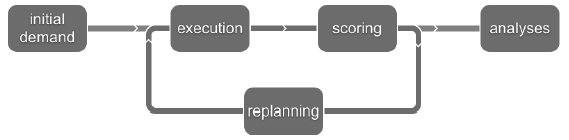
\includegraphics[width=0.8\textwidth]{img/simulation_stages}
	\caption{Schemat etapów symulacji MATSim}
	\label{fig:schemat_symulacji}
\end{figure}

Etap \textit{initial demand} zajmuje się przygotowaniem planów dnia agentów. Podczas tego stadium, wczytany zostaje pełny zestaw agentów wraz z~ich planami dnia, co najmniej jednym dla każdego agenta. Taki plan składa się z~listy aktywności (na przykład bycie w~domu, praca), podróży (składa się na to również wybór środka transportu) oraz informacji pobocznych (jak czas wyjścia z~danego miejsca) i~dokładnych rozkładów tras. Plan opisuje \textit{intencje} agenta. Jeżeli agent przyjmie zbyt optymistyczne założenia dotyczące na przykład przejazdu do pracy i~utknie w~korku lub spóźni się na autobus, możliwe jest, że plan nie zostanie zrealizowany zgodnie z~wcześniejszymi założeniami.

Etap \textit{execution} jest również nazywany \textit{mobility simulation - symulacją transportu}. W~tej fazie plany agentów zostają uruchomione wraz z~reprezentacją świata fizycznego. Oznacza to przemieszczanie agentów wraz z~ich pojazdami po sieci drogowej (w~rzeczywistości infrastrukturze miasta). Podczas tego etapu plany agentów oddziałują na siebie oraz wpływają na symulowaną rzeczywistość. Jeżeli zbyt wielu agentów wybierze jedną drogę w~tym samym czasie, tworzą się ,,korki'' na symulowanych drogach. Dlatego agenci planują swoje \textit{intencje} na dany dzień, jednak nie są w~stanie zaplanować dokładnie przebiegu swojego dnia.

Etap \textit{scoring} następuje po zakończeniu symulacji i~jego głównym celem jest ocena agentów na podstawie przebiegu ich akcji w~ciągu dnia. Funkcja oceniająca jest w~pełni konfigurowalna, jednak główną zasadą jest zwiększanie wyniku agenta  za czas spędzony podczas jego aktywności oraz pomniejszanie go za czas spędzony w~podróży. Zatem najwyższe wyniki uzyskają agenci omijający korki i~wykorzystujący maksymalnie czas na zaplanowane akcje.

Etap \textit{replanning} jest najważniejszą fazą symulacji. W~tym punkcie agenci ,,wyciągają wnioski'' ze swojego dnia i~starają się nie popełnić tych samych błędów, wciąż dążąc do lepszego wyniku. Typowym przykładem takich zmian może być zmiana czasów zakończenia swoich planowanych akcji, zmiana środka transportu lub wybranej drogi. Modyfikacje te są dokonywane przez moduły strategii (\textit{ang. Strategy Modules}).

Etap \textit{analysis} jest ostatnią fazą symulacji i~wykorzystywany jest dla przedstawienia wyników wydajnościowych uzyskanych podczas jej trwania. Mogą to być na przykład takie dane jak typy wybieranego transportu, przebyte kilometry, średni dystans i~czas, zależnie od godzin i~trybów podróży. 

W skrócie, dla zadanej liczby uruchomień symulacji powtarzany jest scenariusz tego samego dnia, dla tego samego zestawu agentów. Ci ostatni, jak zostało wspomniane, po każdym uruchomieniu są oceniani i~na podstawie poprzednio uzyskanych wyników, w~kolejnej iteracji próbują swoje wyniki polepszyć. Działanie symulacji jest oczywiście nierealne, ponieważ agenci codziennie ,,przeżywają'' ten sam dzień, próbując jak najlepiej dopasować swój plan transportu do panującej sytuacji na drodze.

\subsection{Symulacja transportu oparta na agentach}\label{rozdz.agenci}
Przy pomocy \textit{MATSim} możliwa jest symulacja ruchu dla codziennych zachowań komunikacyjnych. W~tym celu wykorzystywani są agenci, reprezentujący pojedyncze jednostki ludzkie. Każdy agent posiada własny plan dnia, pracę i~cele dodatkowe, które realizuje według swojego uznania. Symulacja zwykle pokrywa cały dzień czynności wykonywanych przez wszystkich agentów jednocześnie. Pozwala to na śledzenie pojedynczych jednostek od momentu wyjścia z~domu do pracy, robienie zakupów i~wieczorny powrót. Celem każdego agenta jest uzyskanie jak najwyższego ,,wyniku'' w~ciągu dnia. Agent zdobywa punkty poprzez realizowanie swoich planów (na przykład: praca, zakupy), natomiast traci je podczas komunikacji lub za spóźnienia.

Agenci potrafią modyfikować swoje początkowe plany, tak by nowe ich warianty pozwoliły im na zdobycie wyższego wyniku. Główne założenie procesu optymalizacji wywodzi się z~algorytmów (co-)ewolucyjnych. Cząstka ,,co'' została dodana ze względu na oddzielność algorytmu genetycznego dla każdego agenta z~osobna, jednak wyniki uzyskanych planów dnia są zależne od całego systemu agentów. 

Poprzez plany dnia, agenci bezpośrednio wymuszają zapotrzebowanie na transport. Pełen zestaw agentów w~danym symulowanym scenariuszu ruchu drogowego nazwano populacją scenariusza.. Populacja zawiera dane w~postaci hierarchicznej struktury (pliku XML), którego przykład został zaprezentowany na listingu~\ref{lst:przykladowa_populacja}.

\begin{lstlisting}[caption=Przykładowy plik populacji scenariusza zawierający plany dnia agentów, label=lst:przykladowa_populacja, mathescape]
<?xml version="1.0" encoding="utf-8"?>
<!DOCTYPE population SYSTEM "http://www.matsim.org/files/dtd/population_v5.dtd">
<population>
	<person id="1">
		<plan selected="yes" score="93.2987721">
			<act type="home" link="1" end_time="07:16:23" />
			<leg mode="car">
				<route type="links">1 2 3</route>
			</leg>
			<act type="work" link="3" end_time="17:38:34" />
			<leg mode="car">
				<route type="links">3 1</route>
			</leg>
			<act type="home" link="1" />
		</plan>
	</person>
	<person id="2">
		<plan selected="yes" score="144.39002">
		$\ldots$
		</plan>
	</person>
</population>
\end{lstlisting}

Struktura tego pliku może zostać opisana w~następujący sposób:
\begin{itemize}
\item Plik zawiera listę agentów symulowanych w~danym scenariuszu.
\item Każdy agent posiada listę swoich planów dnia, które będzie realizować.
\item Każdy plan składa się z~listy typów aktywności i~tras.
\end{itemize}

Podczas każdej iteracji symulacji, dla każdego agenta zostaje wybrany jeden plan. W~przypadku posiadania więcej niż jednego planu przez agenta, w~procesie optymalizacji może zostać wybrany inny plan w~kolejnej iteracji symulacji. Lista typów aktywności i~tras opisują dokładnie planowane przez agenta wykonywane akcje. Każda czynność ma przypisane swoje miejsce wykonywania, którym może być dany węzeł sieci (ulica) lub pozycja na mapie znajdująca się pod wskazanymi koordynatami (budynek). Trasa opisuje dokładny plan agenta, w~jaki sposób zamierza dotrzeć z~jednego miejsca do drugiego. Opis ten zawiera sposób komunikacji: auto, autobus, rower lub droga pokonywana pieszo. Na szczęście, do poprawnego wykonania symulacji wystarczające jest podanie jedynie niektórych parametrów:

\begin{itemize}
\item Każdy agent musi posiadać co najmniej jeden plan.
\item Plan nie musi być domyślnie wybrany ani nie musi posiadać obliczonego wyniku.
\item Miejsce odbywania się aktywności wystarczy by było opisane jedynie przez koordynaty, w~którym się znajduje.
\item Planowane aktywności muszą mieć oznaczony czas zakończenia.
\item Trasa musi posiadać jedynie zdefiniowany sposób transportu, bez obliczonej dokładnej trasy dotarcia do celu.
\end{itemize}

\section{Ustawienia symulatora transportu}\label{rozdz.ustawienia_symulatora}
Ważną kwestią przed realizacją samego zadania optymalizacji jest dobór jego ustawień.~Część z~nich jest oczywiście stała lub nie ma wpływu bezpośrednio na obliczenia. Kluczową rolę dla ostatecznego wyniku odgrywają jednak parametry samej symulacji.

Większość ustawień została niezmieniona, pochodzi więc od twórców przykładu Sioux Falls, przybliżonego w~podrozdziale~\ref{rozdz.opis_siouxfalls} Symulator zawiera jednak ważny parametr, a~mianowicie ilości iteracji. Zgodnie z~założeniami symulatora, podczas każdej kolejnej iteracji, celem agenta jest zwiększenie jego średniego wyniku. Dąży on zatem do optymalizacji swoich planów dnia względem warunków na drodze. Krok ten został już opisany w~sekcji \ref{rozdz.agenci} Przekłada się to bezpośrednio również na średni czas podróży każdego agenta. Twórcy zalecają stosowanie wysokich liczb iteracji, dla uzyskania jak najlepszych wyników. Operacje te są jednak czasochłonne. Na rysunku \ref{fig:symulacja_czas} przedstawiony został graf czasu uruchomienia symulacji jednej sieci dla stu iteracji. Podczas symulacji wykorzystywana była domyślna sieć miasta Sioux Falls.

\begin{figure}[htbp]
	\centering
	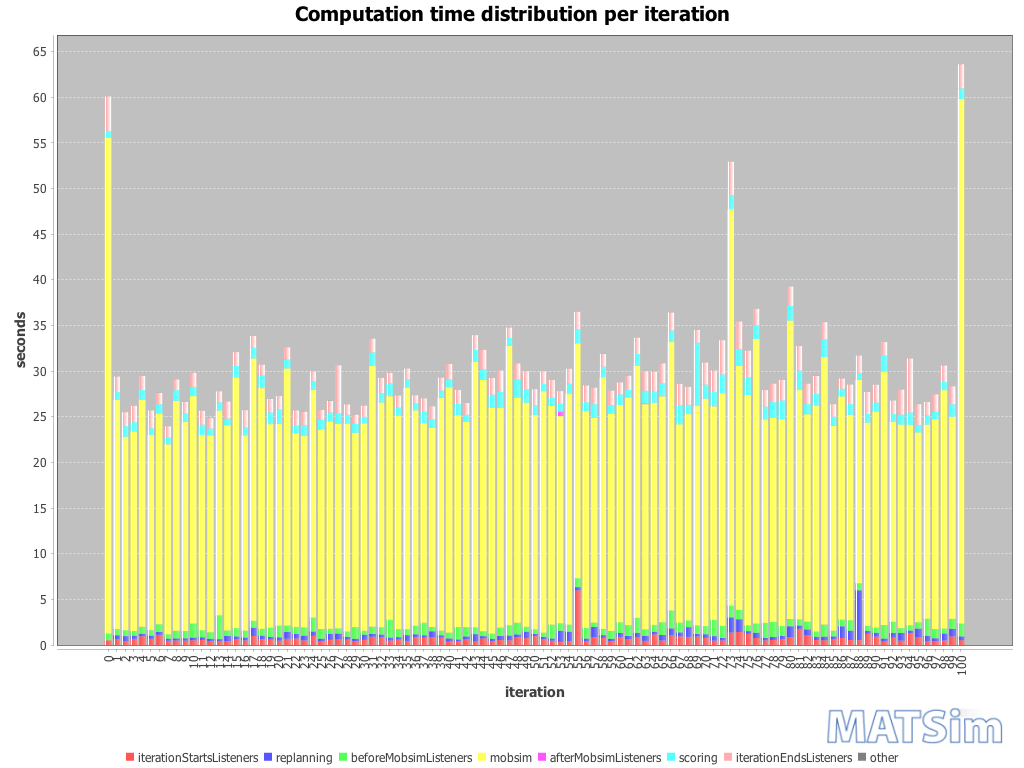
\includegraphics[width=\textwidth]{img/def_stopwatch}
	\caption{Graf czasu trwania symulacji \textit{MATSim} dla stu iteracji}
	\label{fig:symulacja_czas}
\end{figure}

Schemat etapów symulacji został przedstawiony w~sekcji~\ref{rozdz.symulacja}. Nazwy procesów z~wykresu w~odniesieniu do wcześniej objaśnionych etapów symulacji to:
\begin{enumerate}
\item \textit{iterationStartListeners} --- \textit{initial demand},
\item \textit{beforeMobSimListeners, mobSim, afterMobSimListeners} --- \textit{execution}, 
\item \textit{scoring} --- \textit{scoring},
\item \textit{replanning} --- \textit{replanning},
\item \textit{iterationEndsListeners} --- \textit{analyses}.
\end{enumerate}

Analizując wykres czasu trwania kolejnych iteracji, na rysunku~\ref{fig:symulacja_czas}, można również odczytać czas całej symulacji, który wyniósł dokładnie $52$ min~$43$ sek.  W~przypadku analizy wielu (setek) sieci, czas więc jest wyraźnie zbyt długi. Przeanalizowano wpływ ilości iteracji na średni czas przejazdu (Rys. \ref{fig:iteracje_czas}). Średni wynik uzyskany przez agentów został natomiast przedstawiony na rysunku \ref{fig:iteracje_wynik}

\begin{figure}[htbp]
	\centering
	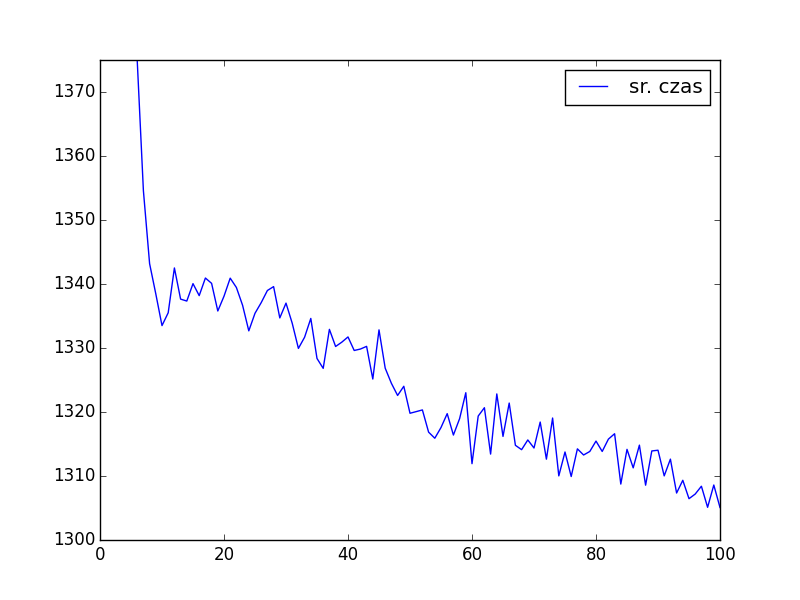
\includegraphics[width=0.85\textwidth]{img/def_iters}
	\caption{Graf średniego czasu przejazdów agentów dla stu iteracji symulacji}
	\label{fig:iteracje_czas}
\end{figure}

\begin{figure}[htbp]
	\centering
	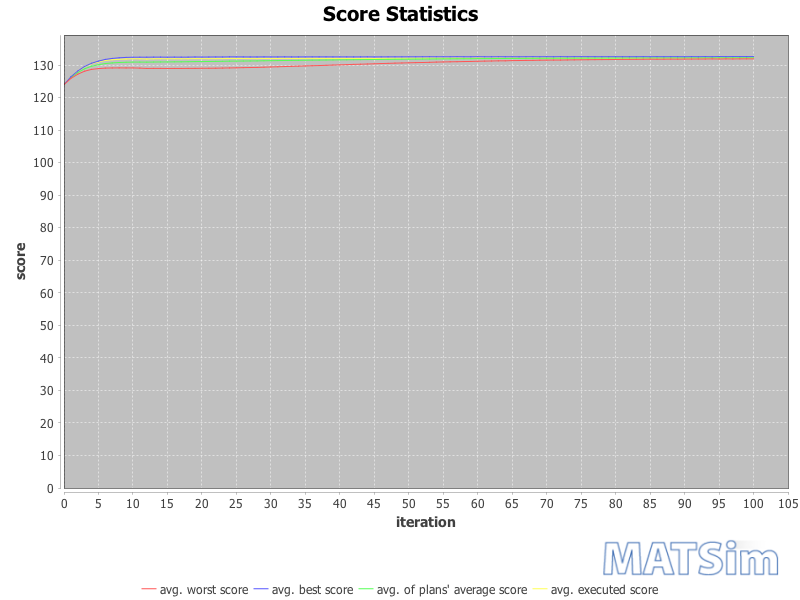
\includegraphics[width=0.85\textwidth]{img/def_scorestats}
	\caption{Graf wyników agentów dla stu iteracji symulacji}
	\label{fig:iteracje_wynik}
\end{figure}

Na rysunkach~\ref{fig:iteracje_czas} i~\ref{fig:iteracje_wynik} widać, że wpływ iteracji, ma największe znaczenie w~początkowych stadiach. W~późniejszych iteracjach zmiana następuje dużo wolniej. Wiąże się to z~wykorzystanym algorytmem, występującym w~fazie \textit{replanning}. Ponadto, analizując rysunek \ref{fig:symulacja_czas} można wnioskować, iż najbardziej czasochłonnym etapem jest etap realnej symulacji ruchu. W~związku z~tym, najlepszym sposobem na ograniczanie czasu potrzebnego do ukończenia obliczeń, jest zmniejszenie ilości iteracji w~symulacji.

Po analizie danych z~rysunków~\ref{fig:iteracje_czas} i~\ref{fig:iteracje_wynik} zdecydowano, by \textbf{w~projekcie użyć $10$ iteracji podczas analizy każdej sieci} Wartość ta optymalnie łączy zalety szybkiego spadku wartości, średnich czasów podróży oraz~czasu potrzebnego na obliczenia. 

\section{Opis badanego miasta Sioux Falls}\label{rozdz.opis_siouxfalls}

Główną zaletą korzystania z~\textit{MATSim}, jest dość pokaźny zbiór danych przykładowych. Jednym z~nich jest materiał zaprezentowany przez twórców aplikacji, który udostępnili w~2013 roku na zgromadzeniu użytkowników platformy~\cite{siux}. Przykład ten dotyczy miasta Sioux Falls w~Południowej Dakocie. Domyślnie scenariusz symulacji ruchu drogowego składa się z:

\begin{itemize}
\item dwóch grup zapotrzebowania bez charakterystyk socjodemograficznych:
\begin{itemize}
\item 68094 agentów z~samochodem oraz korzystających z~transportu publicznego,
\item 40877 agentów posiadających samochód.
\end{itemize}
\item dostosowanej sieci drogowej miasta Sioux Falls,
\item transportu publicznego razem z~rozkładem jazdy,
\item przykładowych miejsc zamieszkania, pracy i~rozrywki.
\end{itemize}

Dostarczony materiał danych jest zbyt obszerny na potrzeby eksperymentu zrealizowanego w~niniejszej pracy. Dostosowano go zatem poprzez usunięcie transportu publicznego oraz wyposażenie każdego agenta we własny samochód. Powyższe modyfikacje znacznie wzmogły ruch w~mieście (co było pozytywnym efektem) i~skróciły obliczenia związane z~symulacjami. Na rysunku~\ref{fig:siouxfalls_siec} przedstawiono sieć miasta odwzorowaną w~postaci grafu. Rysunek został obrócony o~$90^{\circ}$ w~lewo, dla zwiększenia jego czytelności. Natomiast na rysunku \ref{fig:siouxfalls_budynki} zaprezentowano rozkład miejsc pracy, domostw i~innych zakładów nałożonych na graf sieci drogowej miasta.

\begin{figure}[htbp]
	\centering
	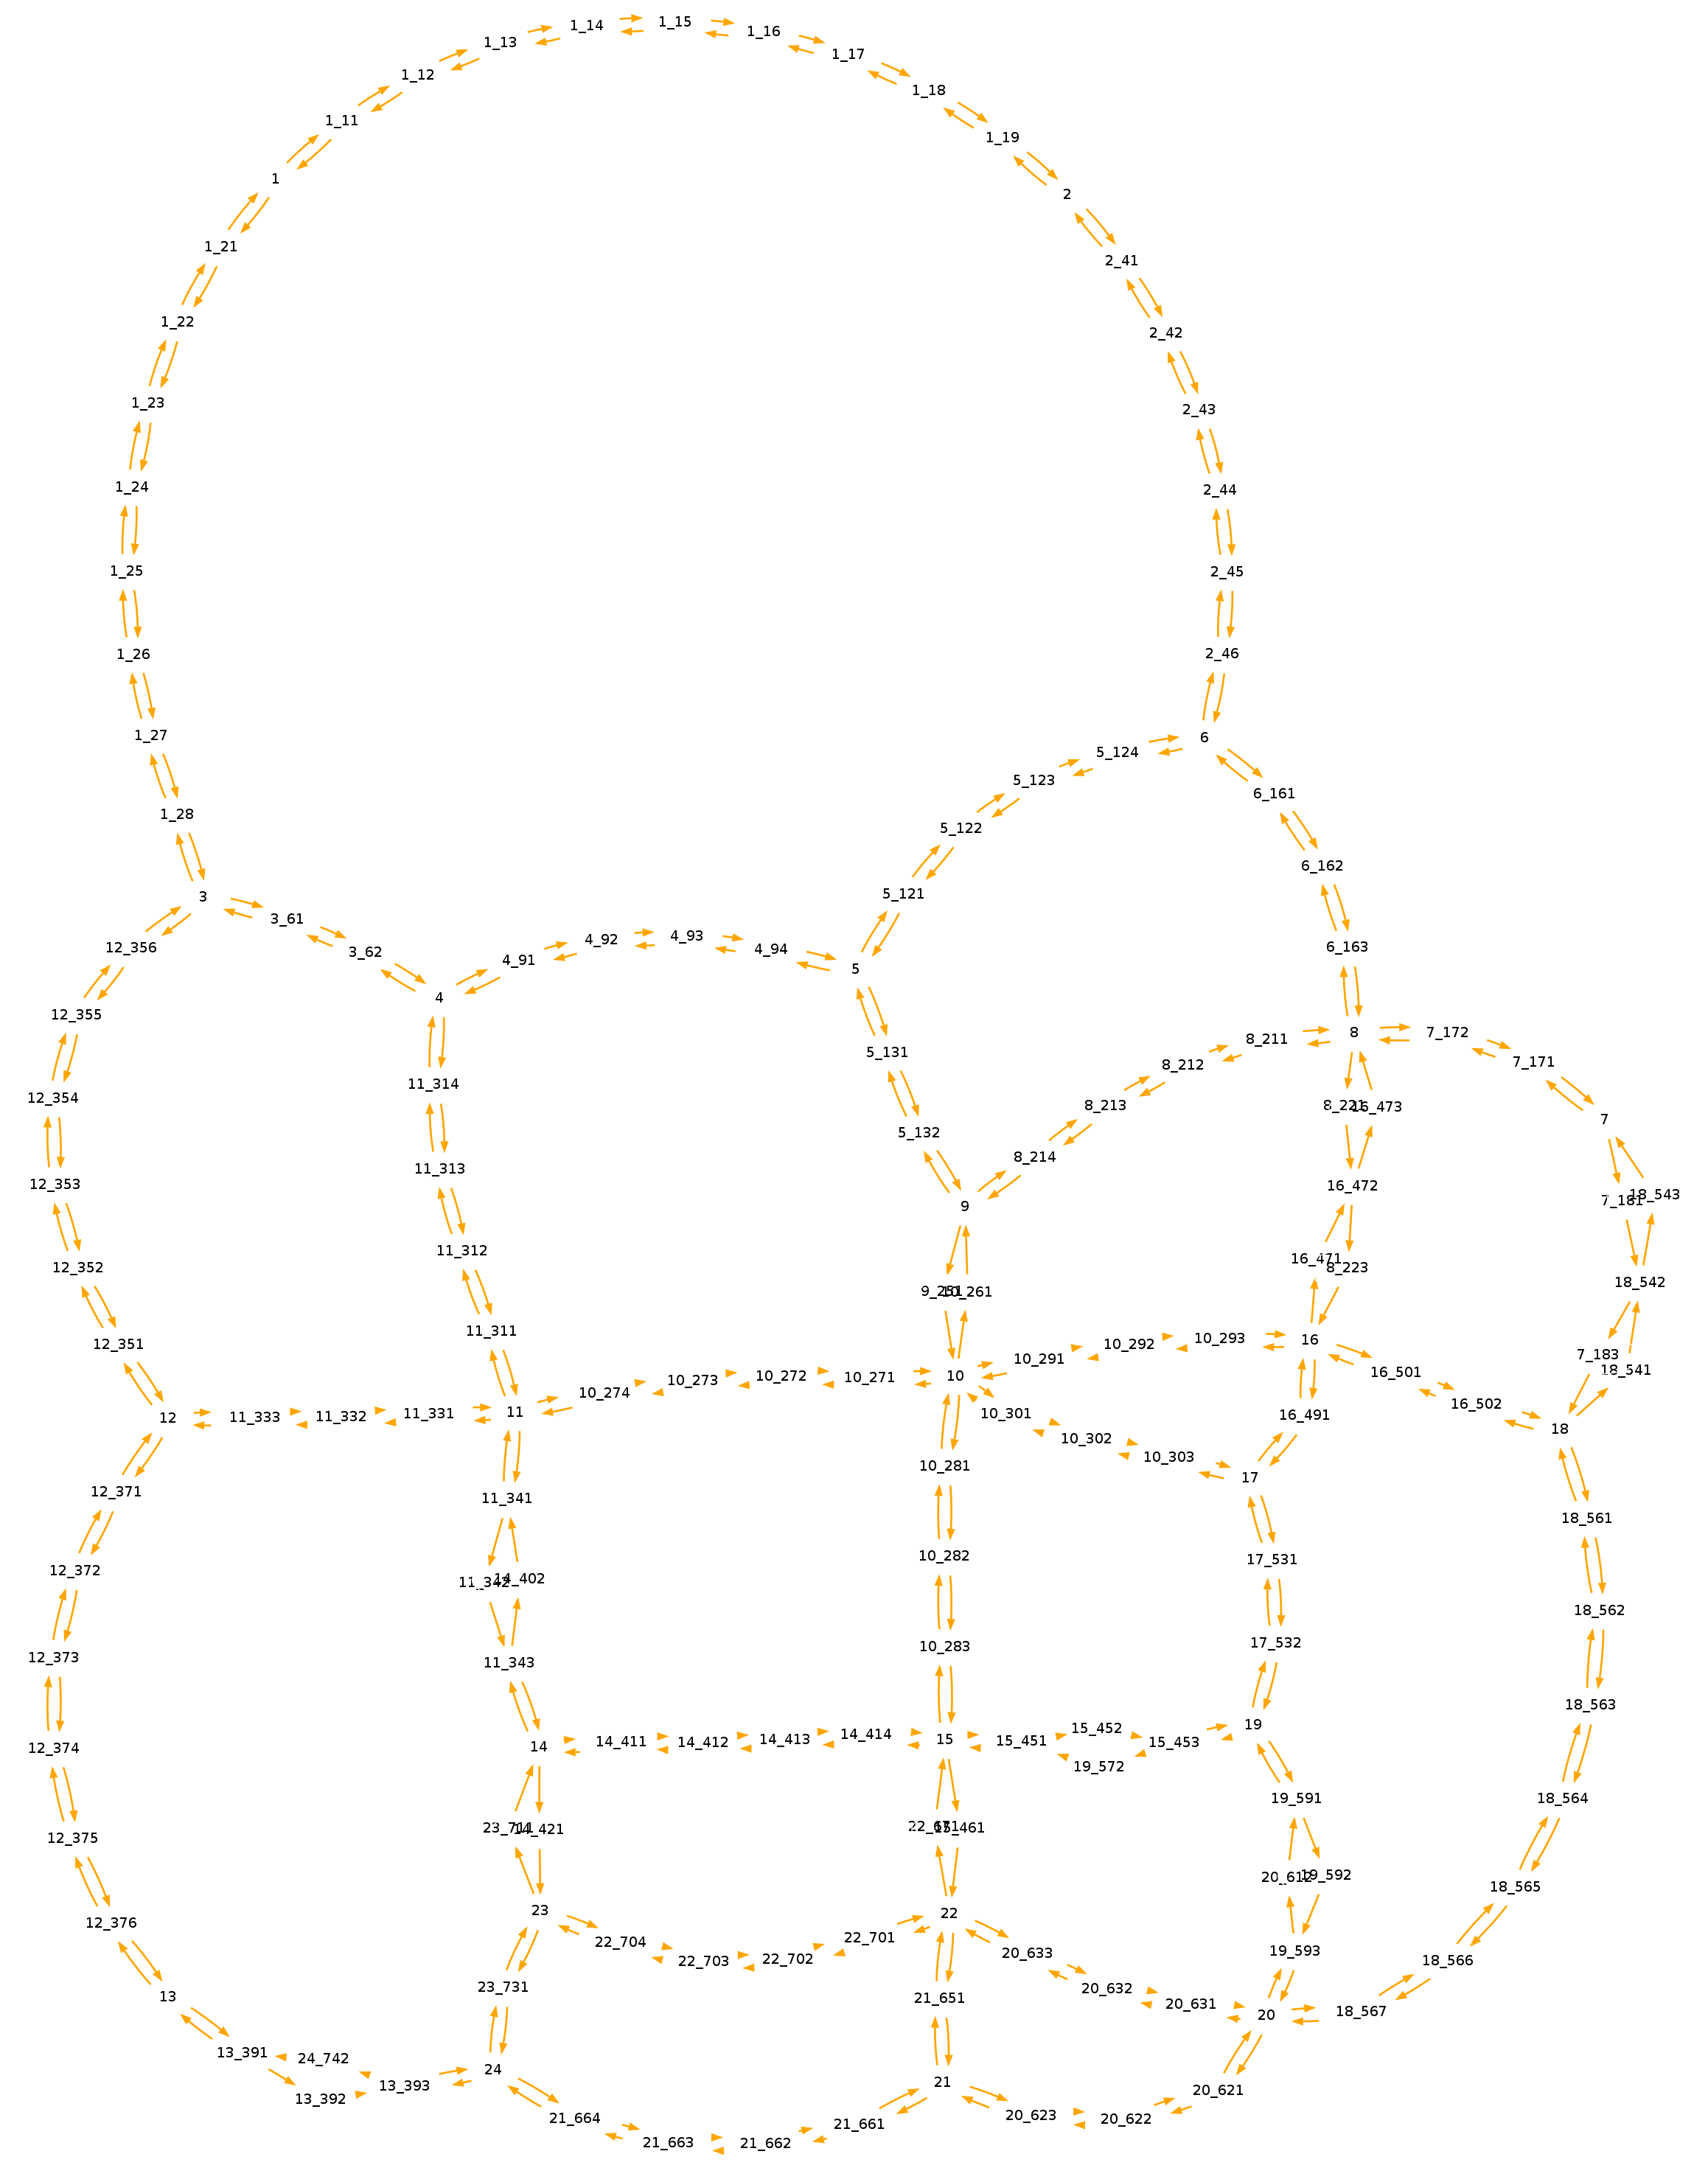
\includegraphics[totalheight=0.560\textheight,angle=90]{img/sioux/network}
	\caption{Graf sieci prezentowanego miasta Sioux Falls} 
	\label{fig:siouxfalls_siec}
\end{figure}

\begin{figure}[htbp]
	\centering
	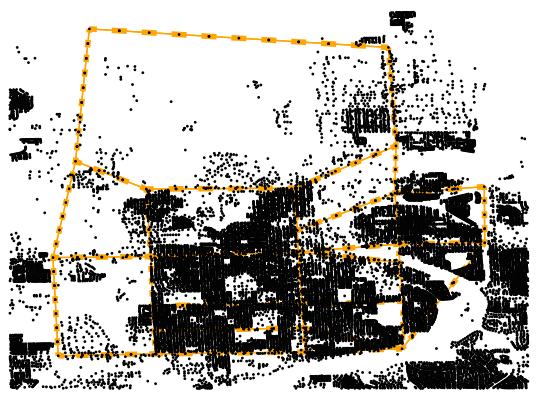
\includegraphics[width=0.8\textwidth]{img/sioux/facilities}
	\caption{Rozkład budynków na grafie miasta Sioux Falls} 
	\label{fig:siouxfalls_budynki}
\end{figure}

Na rysunku~\ref{fig:siouxfalls_natezenie_1} i~\ref{fig:siouxfalls_natezenie_2} zaprezentowano ruch drogowy w~najbardziej intensywnych godzinach dnia, to jest w~godzinach szczytu. Jest on przedstawiony jako natężenie ruchu na każdej krawędzi (ulicy), poprzez odniesienie go do możliwości przepustowości każdego węzła. Kolor zielony oznacza małe obciążenie, żółty - średnie a~czerwony wysokie natężenie ruchu w~tym miejscu. Rysunki zostały obrócone o~$90^{\circ}$ w~lewo, dla zwiększenia ich czytelności. 

\begin{figure}[htbp]
	\centering
	%bottom right top left
	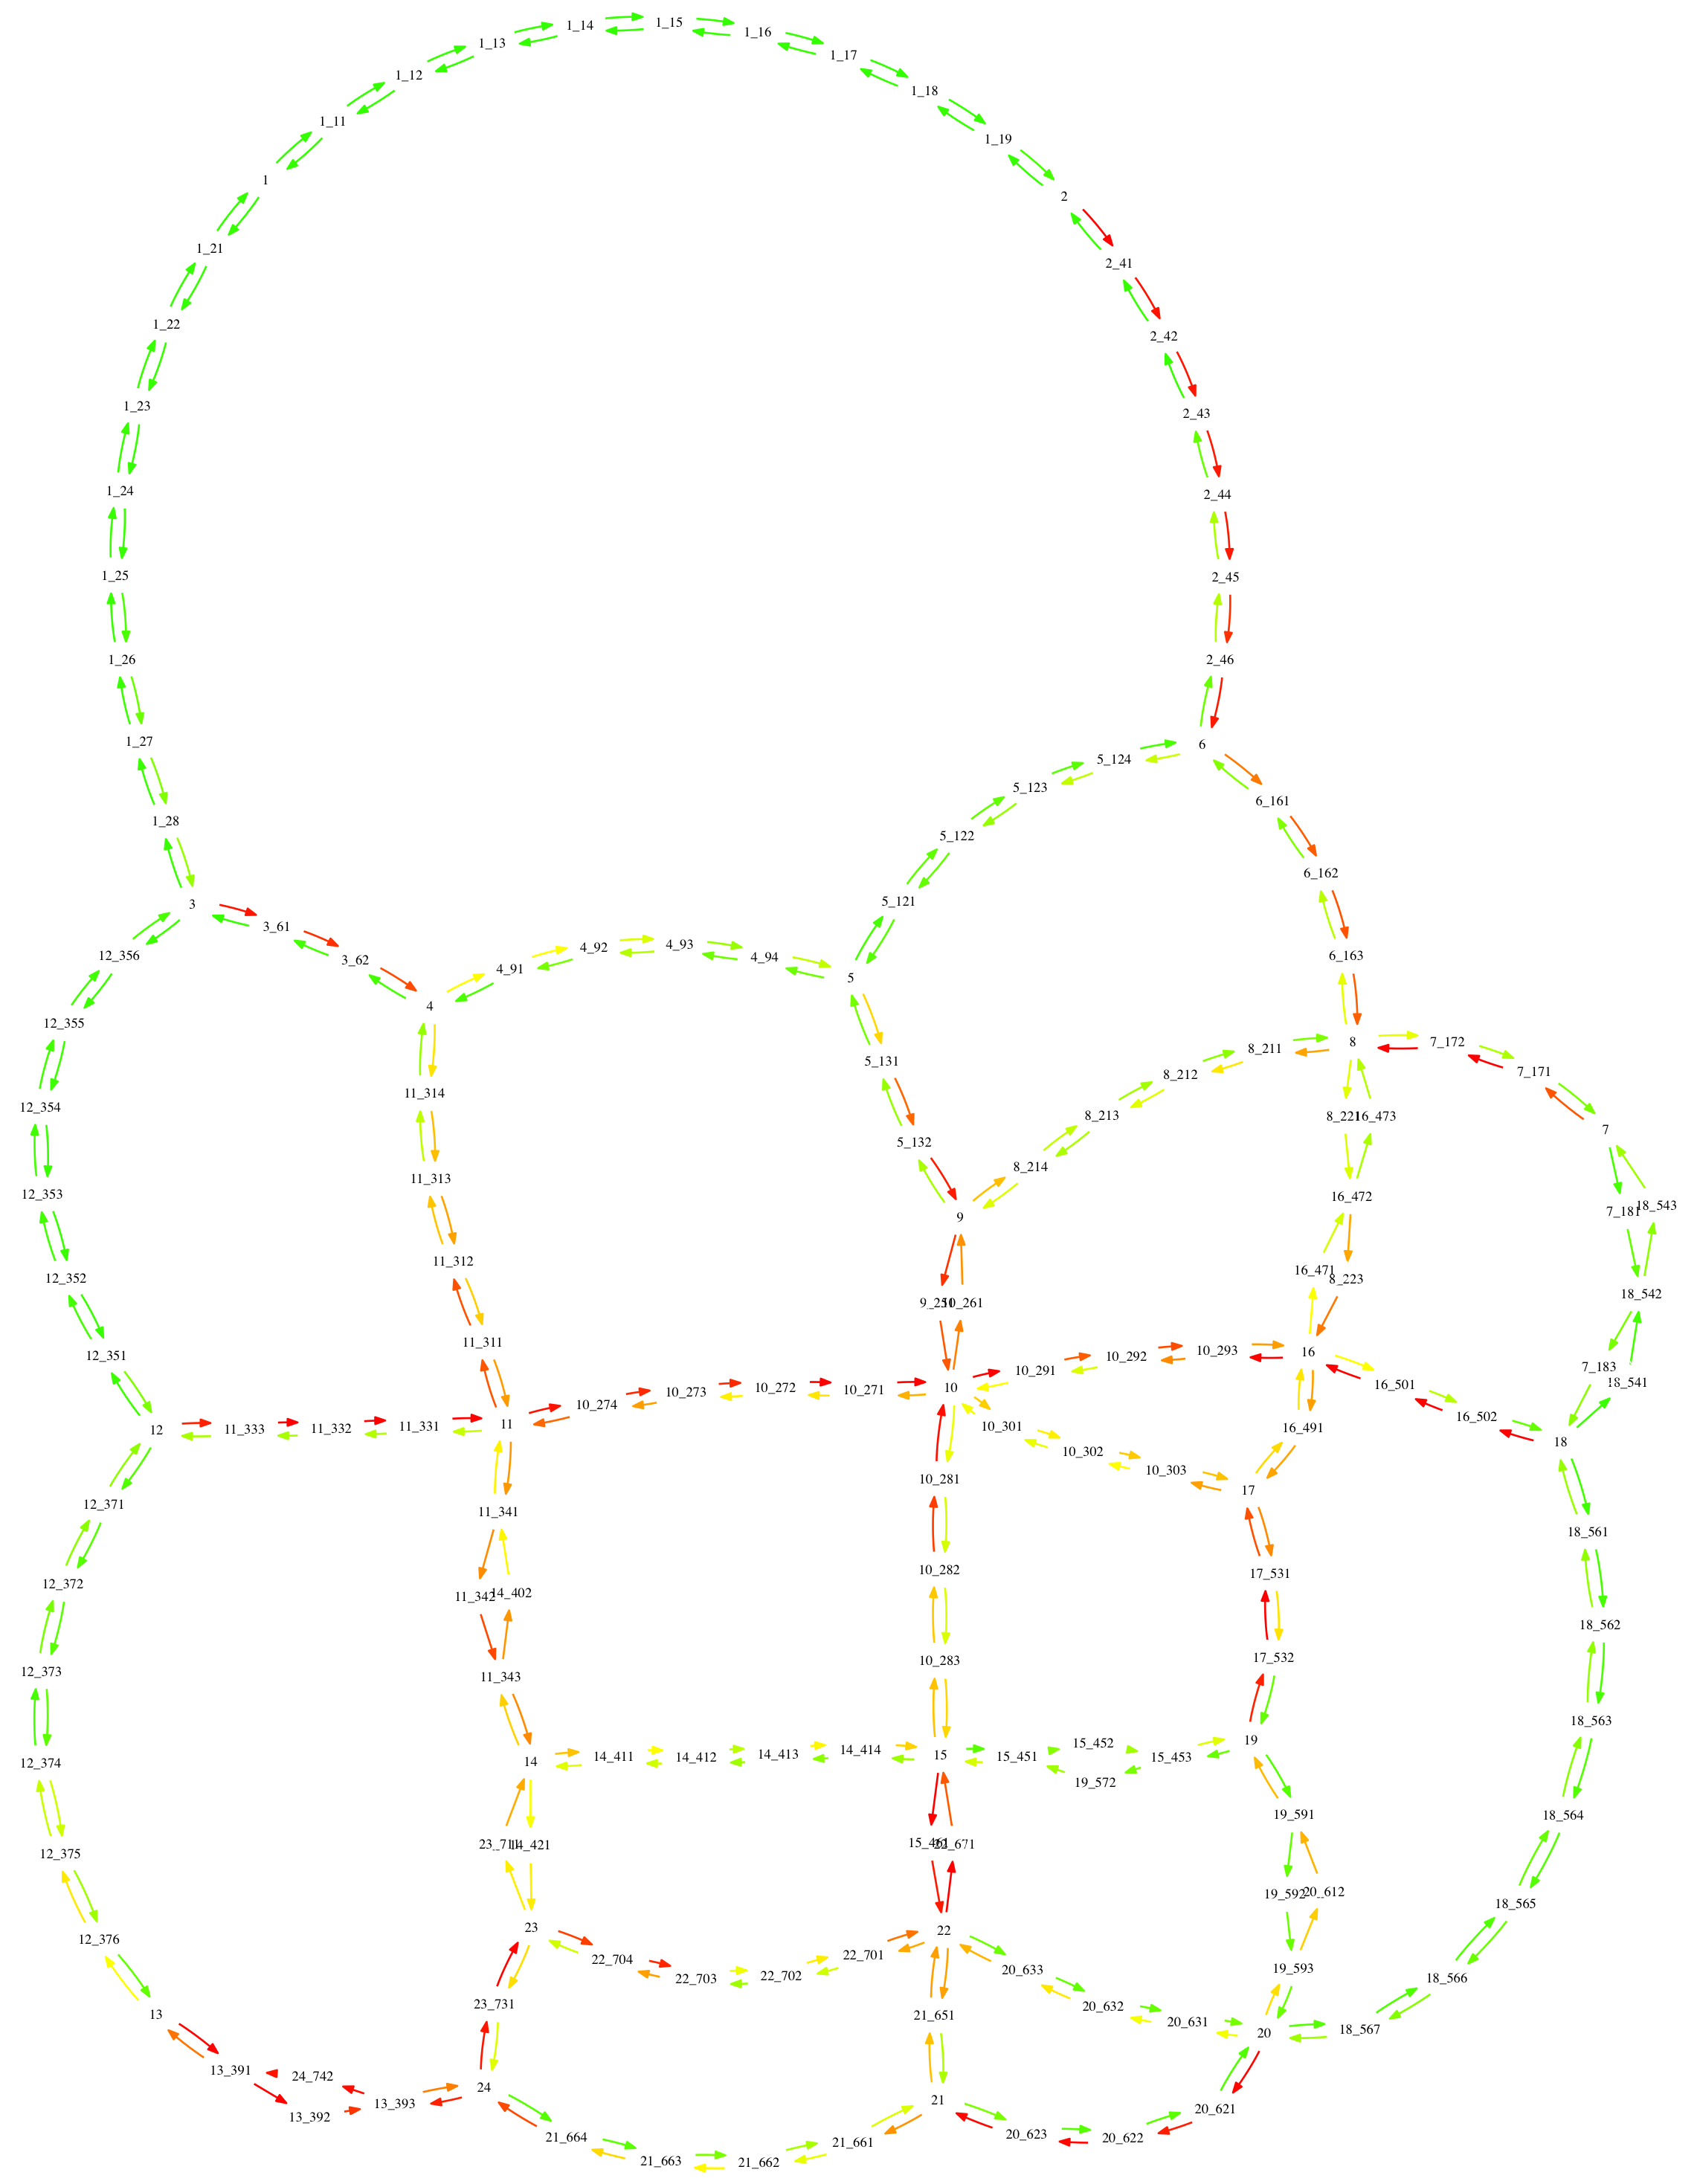
\includegraphics[totalheight=0.560\textheight, angle=90]{{{img/sioux/graph6.00-7.00}}}
	\caption{Natężenie ruchu w mieście Sioux Falls w godzinach 6.00 - 7.00} 
	\label{fig:siouxfalls_natezenie_1}
\end{figure}

\begin{figure}[htbp]
	\centering
	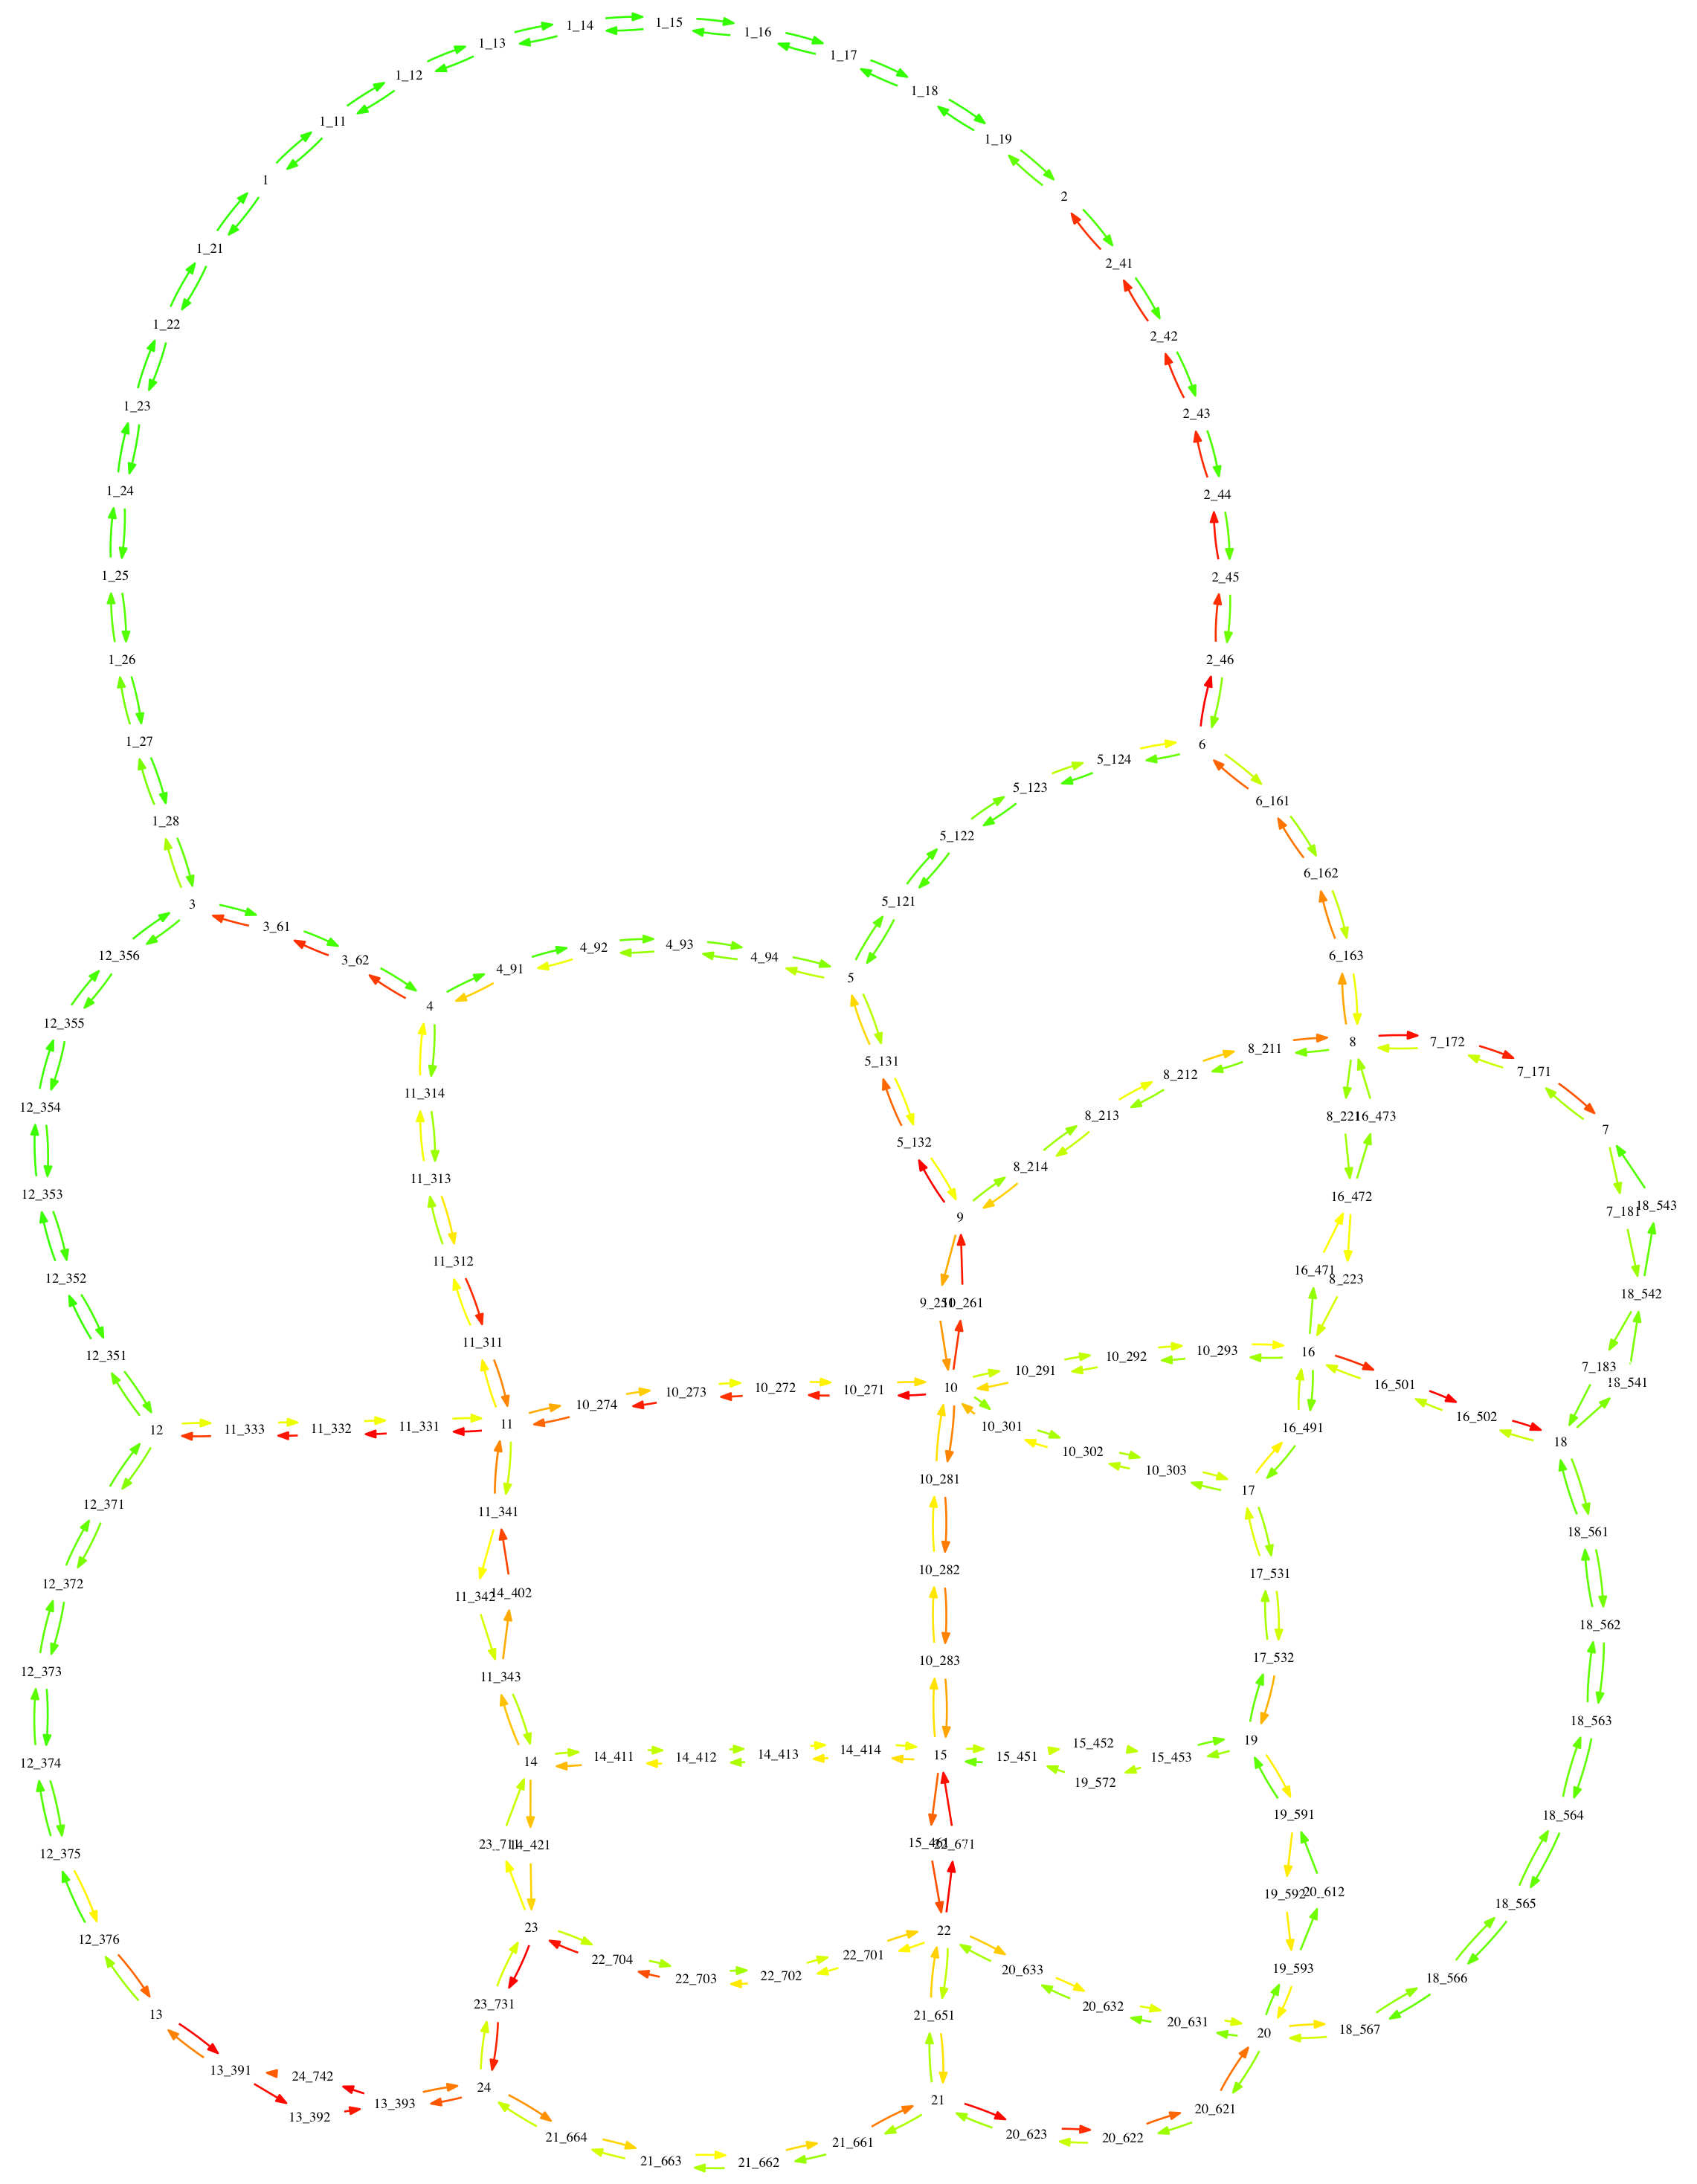
\includegraphics[totalheight=0.560\textheight, angle=90]{{{img/sioux/graph16.00-17.00}}}
	\caption{Natężenie ruchu w mieście Sioux Falls w godzinach 16.00 - 17.00} 
	\label{fig:siouxfalls_natezenie_2}
\end{figure}

W powyższym rozdziale opisano wybrany system symulacji transportu ruchu drogowego MATSim wraz z~jego ustawieniami. Przedstawiono ustawienia symulatora oraz przykładowe miasto wykorzystane w~badaniach prezentowanych w~części praktycznej. W~kolejnym rozdziale zostaje omówiona teoretyczna strona projektu GRoNO, prezentując jego biblioteki oraz konfigurację uruchomienia.

\chapter{Przedstawienie projektu GRoNO}\label{rozdz.grono-teoria}
W niniejszym rozdziale opisane zostają technologie informatyczne, które zostały użyte podczas tworzenia rozwiązania GRoNO.~Wyjaśniono działanie kolejnych elementów projektu oraz przedstawiono użyte zewnętrzne biblioteki. Opisany został również sposób wdrożenia rozwiązania jak i~dane użyte podczas zrealizowanych badań.

\section{Technologie i~metodologie programistyczne}
Użyte w~projekcie technologie programistyczne są poniekąd wymuszone przez języki programowania, w~jakich zostały stworzone wykorzystywane rozwiązania pomocnicze. W~przypadku symulatora \textit{MATSim} jest to język \textbf{Java}. Język \textbf{Python} został wykorzystany głównie ze względu na wykorzystaną bibliotekę \textit{NetworkX}, obsługującą grafy.

\section{Biblioteka komponentów algorytmów genetycznych}
Projekt \textbf{The Apache Commons} jest tworzony przez \textit{Apache Software Foundation}. Głównym celem projektu jest stworzenie wolnego oprogramowania do wielokrotnego użytku w~języku \textit{Java}. Projekt podzielony jest na trzy główne części: \textit{proper}, \textit{sandbox}, i~\textit{dormant}~\cite{math}.

Część \textit{ Apache Commons Proper} jest dedykowana do tworzenia i~utrzymania komponentów wielokrotnego użycia, w~której programiści mogą pracować wspólnie nad projektami współdzielonymi ze społecznością. Celem twórców jest tworzenie indywidualnych elementów posiadających jak najmniej zależności pomiędzy zewnętrznymi rozwiązaniami. Dzięki temu możliwe jest stworzenie niezależnych, integralnych modułów. Dodatkowo, ambicją projektu jest zapewnienie jedynie stabilnych elementów, zapewniających wsteczną kompatybilność.

W przypadku głównej części\textit{ Apache Commons Proper} wyróżnia się wiele modułów różniących się funkcjonalnością i~celem. \textit{Apache Commons Math} jest modułem zapewniającym rozwiązania problemów głównie matematycznych i~statystycznych. Znajduje się w~nim implementacja podstawowej formy algorytmu genetycznego, którą rozszerzono w~niniejszej pracy dyplomowej.

Na rysunkach~\ref{fig:class_math3_1} i~\ref{fig:class_math3_2} zaprezentowane zostały wykorzystane w~projekcie GRoNO klasy z~projektu \textit{Apache Commons Math} 

\begin{figure}[htbp]
	\centering
	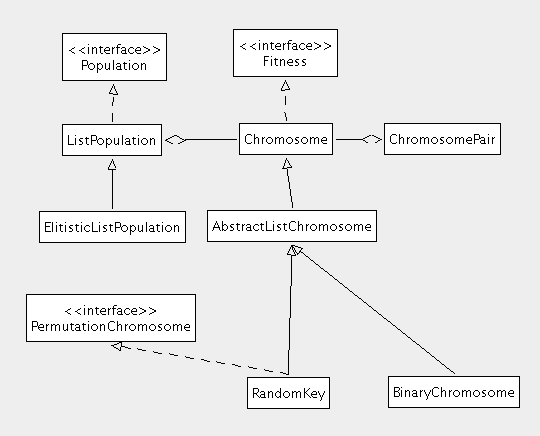
\includegraphics[width=0.85\textwidth]{img/math3-1}
	\caption{Diagram wybranych klas pakietu \textit{Apache Math Genetics}, część 1}
	\label{fig:class_math3_1}
\end{figure}

Analizując klasy dostarczone przez pakiet na rysunku~\ref{fig:class_math3_1} wyraźnie widać jedynie podstawową strukturę algorytmu genetycznego. Biblioteka dysponuje oczywiście klasą \textit{BinaryChromosome}, który idealnie spełnia swoje zadanie w~klasycznym algorytmie genetycznym. Dodatkowo, na diagramie uwzględniono klasę \textit{ElitisticListPopulation}, odpowiadająca elitarnej strategii selekcji opisywanej w~podrozdziale \ref{sec:selekcja}. Dostarczone klasy w~wygodny sposób pozwalają programiście na dołączenie własnej funkcji dostosowania poprzez implementację interfejsu \textit{Fitness}.

\begin{figure}[htbp]
	\centering
	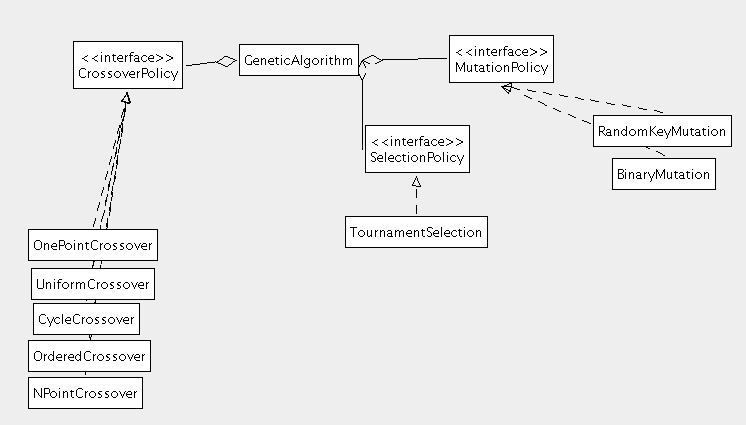
\includegraphics[width=0.85\textwidth]{img/math3-2}
	\caption{Diagram wybranych klas z pakietu \textit{Apache Math Genetics}, część 2}
	\label{fig:class_math3_2}
\end{figure}

Na diagramie zaprezentowanym na rysunku~\ref{fig:class_math3_2} przedstawiono klasy odpowiadające za sam przebieg działania algorytmu genetycznego. Znalazły się tutaj podstawowe klasy odpowiadające metodom omawianym w~podrozdziale \ref{sec:selekcja}, takie jak \textit{BinaryMutation} - klasyczna mutacja, \textit{TournamentSelection} - selekcja turniejowa oraz parę klas dotyczących krzyżowania. W~projekcie GRoNO wykorzystano krzyżowanie jednopunktowe, które zostało zrealizowane w~klasie \textit{OnePointCrossover}.

Oczywiście w~projekcie wiele klas podstawowych zostało przeciążonych tak by realizowały niektóre specyficzne aspekty projektu GRoNO.~Schemat działania samego algorytmu został jednak zachowany.

\section{Biblioteka do obsługi grafów}\label{rozdz.obsluga_grafow}
Ponieważ moduł do wizualizacji rozwiązań \textit{MATSim} nie spełniał  oczekiwań zarówno pod względem wydajności, jak i~stabilności zdecydowano się na stworzenie autorskiej jego implementacji. W~tym celu wykorzystano projekt \textbf{NetworkX}.~Jest to biblioteka wykonana w~języku \textit{Python}, stworzona z~myślą o~grafach i~sieciach. Jest ona dostarczana jako darmowe oprogramowanie na licencji \textit{BSD-new}~\cite{networkx}. Wybór biblioteki oparty był głównie na dostarczanych przez nią gotowych implementacjach, które w~pełni pokrywały się z~wymaganiami projektowymi.

Przede wszystkim bardzo wygodna w~użyciu była pełna integracja biblioteki z~popularną biblioteką graficzną \textit{matplotlib}, skupiającą się na rysowaniu wykresów oraz grafach. Dzięki temu połączeniu struktury grafów tworzone w~NetworkX mogły być wizualizowane bez konieczności konwersji. 

Ponadto biblioteka zawiera gotowe klasy związane z~różnymi typami grafów, w~tym grafami skierowanymi opisywanymi w~podrozdziale~\ref{sec:podstawy_grafy}. Działając na gotowej strukturze można w~pełni korzystać z~wbudowanych algorytmów do analizy i~przeszukiwania grafów. Metody te zostały opisane w~podrozdziale \ref{sec:przeszukiwanie_grafow} oraz \ref{sec:graf_spojny}.

\section{Uruchomienie obliczeń w~chmurze}
Ze względu na duże wymagania sprzętowe obliczeń, a~zarazem ograniczoną przenośność rozwiązania z~powodu skorzystania z~języka \textit{Python}, zdecydowano się na usprawnienie rozwiązania. Wykorzystując system \textit{Linux Ubuntu} stworzono maszynę wirtualną, spełniającą wszystkie wymagania do uruchomienia aplikacji. Dzięki temu stało się możliwe wykorzystanie innych komputerów oprócz tego, na którym zostało stworzone rozwiązanie. Podczas badań wykorzystywany był system \textbf{Linux Ubuntu~12.04~LTS}\cite{ubuntu}.

Korzystając z~systemu opisanego powyżej, dzięki któremu projekt jest możliwy do zainstalowania na innych maszynach, do obliczeń wykorzystano zewnętrznego dostawcę mocy obliczeniowej. Przy wyborze decydującym czynnikiem była cena rozwiązania, co w~przypadku chmury\textbf{ Microsoft Azure}~\cite{azure}, pozwoliło na darmowe rozwiązanie\footnote{Dzięki darmowemu okresowi próbnemu.}. Do wyboru użytkownik posiada dość szeroką gamę konfiguracji, które może dostosować idealnie do swoich potrzeb. W~przypadku poniższego projektu kluczowymi aspektami była ilość niezależnych wątków obliczeniowych. Z~sekcji maszyn wirtualnych Linux, do projektu najlepiej nadawała się warstwa podstawowa, przeznaczona do wystąpień ogólnego zastosowania. Jest to ekonomiczna opcja dla obciążeń związanych z~tworzeniem aplikacji, serwerów testowych i~innych aplikacji, które nie wymagają równoważenia obciążeń, automatycznego skalowania i~maszyn wirtualnych korzystających z~dużej ilości pamięci. Na rysunku~\ref{fig:azure_dostepne_opcje} przedstawiono dostępne rozwiązania. W~pracy wykorzystywana została opcja \textit{A4}.

\begin{figure}[htbp]
	\centering
	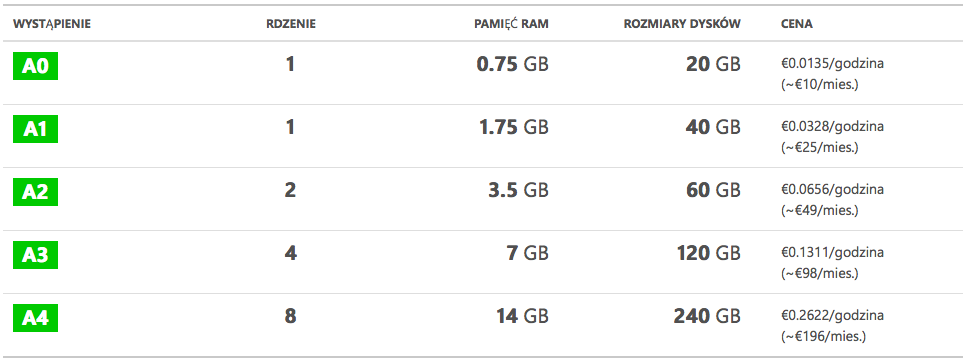
\includegraphics[width=0.8\textwidth]{img/azure_opcje}
	\caption{Dostępne konfiguracje warstwy podstawowej chmury Microsoft Azure}
	\label{fig:azure_dostepne_opcje}
\end{figure}

\section{Obsługa projektu GRoNO}\label{rozdz.konfiguracja_GRoNO}
Ponieważ przeprowadzane w~ramach projektu obliczenia wymagają wiele czasu, zdecydowano się na pominięcie interfejsu użytkownika przy projektowaniu aplikacji. Całość jest obsługiwana przez plik konfiguracyjny, który zostaje wczytany na początku działania programu i~za jego pomocą kontrolowany jest przebieg obliczeń.~Przykładowy plik konfiguracyjny z~opisem jego funkcji przedstawiono na listingu~\ref{lst:przykladowy_config}. Pomimo dwóch osobnych technologii, w~których został wykonany projekt GRoNO, są one od siebie zależne. Całość jest obsługiwana przez część wykonaną  w~języku \textit{Java}, skrypty w~języku \textit{Python} jedynie wspierają niektóre procesy. 

\lstinputlisting[language=Xml, caption=Plik konfiguracyjny projektu GRoNO, label=lst:przykladowy_config]{img/config.xml} 

Analizując listing~\ref{lst:przykladowy_config} można wyróżnić trzy podstawowe grupy konfiguracyjne dostępne w~projekcie GRoNO:
\begin{itemize}
\item project,
\item scenario,
\item genetics.
\end{itemize}

Grupa \textit{project} odpowiada za główne ustawienia całego projektu, w~\textit{scenario} znajdują się ustawienia dotyczące symulacji przeprowadzanej przez \textit{MATSim}, natomiast sekcja \textit{genetics} zawiera ustawienia dotyczące algorytmu genetycznego.

Opcje dostępne w~grupie \textit{project} są następujące:
\begin{itemize}
\item \textit{name} --- nazwa projektu, używana jako katalog wyjściowy,
\item \textit{output dir} --- katalog, gdzie zapisano wyniki optymalizacji sieci drogowych,
\item \textit{threads} --- ilość wątków, które mają być użyte podczas symulacji transportu ruchu drogowego,
\item \textit{log level} --- poziom logowania \textit{Log4J}\footnote{zewnętrzna biblioteka do logowania, dostępne poziomy: DEBUG, INFO, WARN, ERROR i~FATAL},
\item \textit{python path} --- ścieżka instalacji języka Python,
\item \textit{python main} --- folder ze skryptami pomocniczymi,
\item \textit{java-path} --- ścieżka instalacji języka Java,
\item \textit{matsim-jar} --- scieżka do biblioteki \textit{MATSim},
\item \textit{matsim-xmx} --- maksymalna pamięć RAM dostępna dla symulatora \textit{MATSim}.
\end{itemize}

Opcje sekcji \textit{scenario} to:
\begin{itemize}
\item \textit{config} --- scieżka dostępu pliku konfiguracyjnego \textit{MATSim},
\item \textit{network} --- scieżka dostępu pliku z~siecią wejściową scenariusza symulacji,
\item \textit{population} --- scieżka dostępu pliku z~populacją scenariusza symulacji,
\item \textit{facilities} --- scieżka dostępu pliku z~budynkami scenariusza symulacji,
\item \textit{iterations} --- ilość iteracji symulacji \textit{MATSim}.
\end{itemize}

Na zakończenie, opcje grupy \textit{genetics} są następujące:
\begin{itemize}
\item \textit{population size} --- rozmiar populacji,
\item \textit{max generations} --- ilość testowanych generacji (warunek stopu),
\item \textit{elitism rate} --- ilość najlepszych chromosomów biorących udział w~kolejnej iteracji,
\item \textit{crossover rate} --- szansa na krzyżowanie osobników z~poprzedniej populacji przed dodaniem ich do kolejnej generacji,
\item \textit{mutation rate} --- szansa na mutację pojedynczego genu wybranych osobników,
\item \textit{tournament rate} --- ilość osobników biorących udział w~turnieju.
\end{itemize}

\section{Struktura plików projektu GRoNO}
Umieszczone na płycie dołączonej do niniejszej pracy źródła pozwalają na odtworzenie pełnego projektu, używając wymienionych wcześniej środowisk programistycznych, Eclipse i~PyDev. Struktura katalogów, w~kolejności alfabetycznej wraz z~krótkim opisem zawartości, jest następująca:

\subsubsection{fakematsim/}
Jest to sztuczna implementacja symulatora \textit{MATSim} pozwalająca na testowanie działania algorytmu genetycznego w~oparciu o~losowe wyniki. Działanie opiera się o~rozpakowanie gotowego katalogu z~wcześniej przygotowanymi obliczeniami oraz podmianę wyniku na losową liczbę. Projekt jest przygotowany w~oparciu o~strukturę projektu \textit{Maven}. Jego skompilowane źródła znajdują się  w~katalogu \textit{matsim}.

\subsubsection{java/}
Tutaj znajduje się główny projekt zarządzający aplikacją obliczeniową. Jest on przygotowany w~oparciu o~strukturę projektu \textit{Maven}. Zawiera przykładowe pliki konfiguracyjne i~przygotowane testy \textit{JUnit} pozwalające na ich bezpośrednie wykorzystanie.

\subsubsection{literature/}
W tym katalogu zostały zebrane wszystkie źródła literaturowe wykorzystane przy tworzeniu pracy.

\subsubsection{matsim/}
Katalog ten zawiera skompilowane wersje symulatora \textit{MATSim} oraz jego falsyfikatu wykorzystywanego podczas testów. Symulator został skompilowany ze źródeł dostępnych na repozytorium głównym projektu\footnote {\url{https://svn.code.sf.net/p/matsim/source/matsim/trunk}}. Drobne modyfikacje dotyczyły tylko parametrów logowania oraz uruchomienia symulatora. Nie zostały dokonane żadne zmiany ingerujące w~przebieg samej symulacji.

\subsubsection{sioux-out/}
Jest to domyślny katalog z~danymi otrzymanymi w~wyniku działania projketu.

\subsubsection{paper/}
Katalog ze źródłami pracy pisemnej w~formacie TeX.

\subsubsection{python/}
Znajdują się tutaj wszystkie wykorzystane w~projekcie skrypty Python wraz z~testami jednostkowymi. Jest to również domyślny katalog wywołań skryptów podczas obliczeń.

\subsubsection{README.md}
Plik zawierający opis instalacji wymaganych przez projekt zależności i~bibliotek na podstawie systemu Linux Ubuntu 12.04 LTS.

\subsubsection{scenarios/}
Zawiera przykładowe scenariusze symulacji transportu ruchu drogowego, które mogą być wykorzystane przy pracy z~symulatorem \textit{MATSim}. Znajduje się tutaj, oprócz wykorzystanego miasta Sioux Falls, Berlin i~Bruksela. Ponadto zawiera parę przykładowych plików konfiguracyjnych symulatora.

\subsubsection{seminar/}
Zawiera prezentację wykorzystaną podczas seminarium dyplomowego, przedstawiającą wstępne założenia projektu.

W powyższym rozdziale opisano technologie informatyczne związane z~projektem GRoNO.~Zaprezentowane zostały biblioteki informatyczne, z~których skorzystano w~trakcie realizacji projektu. Objaśniono konfigurację potrzebną do uruchomienia projektu GRoNO oraz opisano strukturę plików załączonej do pracy płyty. W~kolejnym rozdziale przedstawione zostaną zoptymalizowane sieci drogowe uzyskane w~wyniku działania programu.

\chapter{Wyniki i~analiza procesu optymalizacji sieci drogowej}\label{rozdz.grono-praktyka} 
W niniejszym rozdziale przedstawiono rezultaty działania projektu GRoNO.~Omówione zostają również parametry konfiguracji wykorzystane podczas tych badań wraz z~ich wartościami. Na zakończenie przedstawiono wyniki optymalizacji przykładowej sieci drogowej. Rezultaty zawierają krótkie omówienie i~analizę.

\section{Użyte ustawienia projektu GRoNO}
Podczas badań przeprowadzonych w~ramach niniejszej pracy dyplomowej wykorzystane zostały ustawienia algorytmu genetycznego zgodne z~listingiem~\ref{lst:wykorzystany_config} Wartości te były dobrane na podstawie doświadczenia nabytego w~trakcie studiów literaturowych. 
	
\begin{lstlisting}[caption=Ustawienia algorytmu genetycznego podczas badań, label=lst:wykorzystany_config]
<genetics>
	<population-size>24</population-size>
	<max-generations>200</max-generations>
	<elitism-rate>2</elitism-rate>
	<crossover-rate>1.0</crossover-rate>
	<mutation-rate>0.8</mutation-rate>
	<tournament-arity>4</tournament-arity>
</genetics>
\end{lstlisting}

Poniżej znajduje się krótkie omówienie opcji sekcji \textit{genetics} oraz wartości poszczególnych ustawień wykorzystanych w~projekcie GRoNO, przedstawionych na listingu~\ref{lst:wykorzystany_config}. Szczegółowe wyjaśnienie pełnej konfiguracji znajduje się w~podrozdziale~\ref{rozdz.konfiguracja_GRoNO}.
\begin{itemize}
\item \textit{population size --- 24} --- rozmiar populacji został dobrany do wielokrotności wątków na serwerze. Ponieważ dostępnych było 8 rdzeni obliczeniowych, wielokrotność pozwalała na zmaksymalizowanie liczby równoległych symulacji \textit{MATSim} podczas pojedynczej generacji.

\item \textit{max generations --- 200} --- warunek stopu był przede wszystkim motywowany ograniczeniem czasowym obliczeń.~Przy liczbie 200 generacji spodziewane obliczenia na serwerze miały zostać zakończone w~przeciągu 48 godzin.

\item \textit{elitism rate --- 2} --- liczba kopiowanych najlepszych rozwiązań do kolejnej generacji była zwiększona do dwóch z~powodu większego rozmiaru populacji (24) i~wybranej metody selekcji osobników.

\item \textit{crossover rate --- 1.0} --- szansa na krzyżowanie osobników z~poprzedniej populacji przed dodaniem ich do kolejnej generacji została ustawiona na 1, by mieć pewność, że zostaną stworzeni nowi osobnicy.

\item \textit{mutation rate --- 0.8} --- szansa na mutację pojedynczego genu wybranych osobników została ustawiona na 0.8 ze względu na dużą przestrzeń przeszukiwań rozwiązania. Takie ustawienie pozwalało maksymalizować szanse znalezienia nowych ekstremów lokalnych.

\item \textit{tournament rate --- 4} --- ilość osobników biorących udział w~turnieju została zwiększona proporcjonalnie do wielkości populacji. Wciąż liczba ta stanowi tylko 15\% z~całej generacji.
\end{itemize}

\section{Wyniki optymalizacji sieci drogowej miasta Sioux Falls}
Wykres przedstawiający zestawienie wyniku najlepszej sieci wyłonionej w~danej iteracji, do wyniku sieci wejściowej przedstawiony został na rysunku~\ref{fig:wynik_globalny} Jego analiza pokazuje, iż bardzo długo najlepsze rozwiązania z~zamkniętymi jakimikolwiek węzłami sieci drogowej uzyskiwały gorsze wyniki globalne niż sieć drogowa z~wszystkimi ulicami dostępnymi. Szczęśliwie po około $150$ iteracjach zostało odnalezione minimum, w~którym zamknięcie pewnych ulic powodowało uzyskanie lepszego wyniku.

\begin{figure}[htbp]
	\centering
	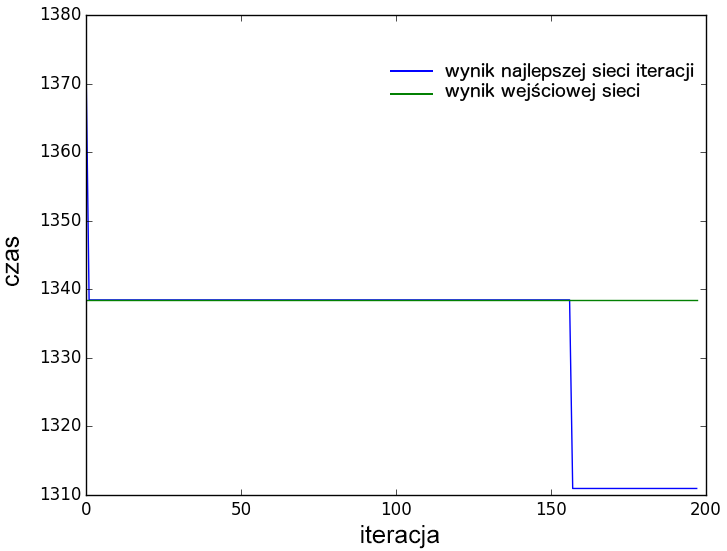
\includegraphics[width=0.85\textwidth]{img/fitness}
	\caption{Wykres zmian najlepszego wyniku iteracji}
	\label{fig:wynik_globalny}
\end{figure}

Ponieważ w~niniejszym projekcie wykorzystany został elitarny model populacji algorytmu genetycznego, powyższy wykres nie przedstawia praktycznie żadnych zmian w~populacji, która została ulepszona. Pojedyncze rozwiązanie, które okazało się najlepszym wynikiem badań posiada jednak  mutacje, które przedstawiają ciekawą wariację tego rozwiązania. Wyniki wszystkich chromosomów były  zachowywane w~bazie danych, dzięki czemu możliwe jest przedstawienie wszystkich rozwiązań spełniających założenia projektowe.

Najlepsze wyniki uzyskane podczas badań przedstawione zostały w~tabeli~\ref{tab:tabela_wynikow} Znajdują się tutaj wszystkie sieci drogowe, które uzyskały wynik lepszy od sieci wejściowej, to jest $1338.4505528474617$. \textbf{Od teraz, sieci te będą nazywane zgodnie z~ich numerem identyfikacyjnym podanym w~pierwszej kolumnie.} Reprezentacja binarna opisuje zamknięte ulice w~grafie. Kolejność ulic reprezentowana przez ciąg binarny jest zawsze taka sama. Została ona ustalona przez algorytm wczytywania grafu w~bibliotece NetworkX (rozdział \ref{rozdz.obsluga_grafow}) i~taka reprezentacja daje mało informacji o~rzeczywistym wyglądzie danej sieci drogowej. Kolumna \textit{wynik sieci} przedstawia średni czas przejazdu agentów w~dziesiątej iteracji symulacji \textit{MATSim}, czyli badany przez nas wynik.

\begin{figure}[htbp]
\centering
\captionof{table}{Tabelaryczna reprezentacja otrzymanych najlepszych sieci drogowych}
\label{tab:tabela_wynikow} 
\begin{tabularx}{\linewidth}{ | l | X | r | }
	\hline
	ID & Reprezentacja binarna & Wynik sieci \\
	\hline
	1 & 011111111111111111111111111111111111111111111 111111111111111111111111111111111111110111111 & 1310.95255617644 \\ \hline
	2 & 011111111111111111111111011111110111111111111 111111111111111111111111111111111111110111111 & 1312.64143383664 \\ \hline
	3 & 011111111111111111111111111111111111111111111 111111111111111111110111111111111111110111111 & 1312.73299250981 \\ \hline
	4 & 011111111111111111111111111111110111111111111 111111111111111111111111111111111111110111111 & 1313.75345975508 \\ \hline
	5 & 011111111111111111111111111111111111111111111 111111111111111111111111111111111111110111101 & 1318.77194744977 \\ \hline
	6 & 011111111111111111111111011111111111111111111 111111111111111111111111111111111111110111111 & 1320.54353227916 \\ \hline
	7 & 011111111111111111111111111111111111111111111 111111111111111111111111111111111111110110111 & 1322.64708120319 \\ \hline
	8 & 011111111111111111111111011111111111111111111 111111111111111111110111111111111111110111111 & 1323.53190464867 \\ \hline
	9 & 011111111111111111111111111111111111111111111 111111111111111111111111111111111111110111110 & 1325.07095470218 \\ \hline
	10 & 01111111111111111111111111111111111111111111 1111111111111111111111110111111111111110111111 & 1327.94727737487 \\ \hline
	11 & 01111111111111111111111111111111111111111111 1111111111111111111111110111111111111110111101 & 1329.46298894305 \\ \hline
	12 & 01111111111111111111111101111111111111111111 1111111111111111111111110111111111111110111111 & 1332.87335631911 \\ \hline
	13 & 01111111111111111111111111111111111111111111 1111111111111111111111111111111111111110111011 & 1334.28138152419 \\ \hline
	14 & 01111111111111111111111111111111111111111111 1111111111111111111111111111111111110110111111 & 1334.48972773749 \\ \hline
	15 & 01111111111111111110111111111111111111111111 1111111111111111111111111111111111111110111111 & 1335.74516109856 \\ \hline
	16 & 01111111111111111111111111111111111111111111 1111111111111111111111111111111111111110111010 & 1335.96306027821 \\ \hline
	17 & 01111111111111111111111111111111111001111111 1111111111111111111111111111111111111110111111 & 1336.65051123529 \\ \hline
\end{tabularx}
\end{figure}%
\clearpage

Na rysunkach~\ref{fig:sioux1} --- \ref{fig:sioux17} zaprezentowano grafy uzyskanych sieci drogowych, wizualizując rozwiązania wymienione w~tabeli \ref{tab:tabela_wynikow} Zostały one przedstawione kolejno oraz oznaczone odpowiednim numerem identyfikacyjnym. \textbf{W celu uproszczenia odnajdowania usuniętych węzłów zostały one zaznaczone czerwonymi prostokątami. Usunięte węzły oznaczone są kolorem czerwonym.}  W~niektórych przypadkach wycięte węzły są trudno widoczne, z~powodu nikłej długości strzałki. Dotyczy to przede wszystkim rysunków: \ref{fig:sioux5}, \ref{fig:sioux7}, \ref{fig:sioux9}, \ref{fig:sioux10}, \ref{fig:sioux11}, \ref{fig:sioux12}, \ref{fig:sioux13}, \ref{fig:sioux14}, \ref{fig:sioux16} Tak, jak w~poprzednich przypadkach, rysunki przedstawiające sieci drogowe zostały obrócone o~$90^{\circ}$ w~lewo. 


\begin{figure}[htbp]
\centering
\begin{tikzpicture}
    \node[anchor=south west] (image) at (0,0)
    {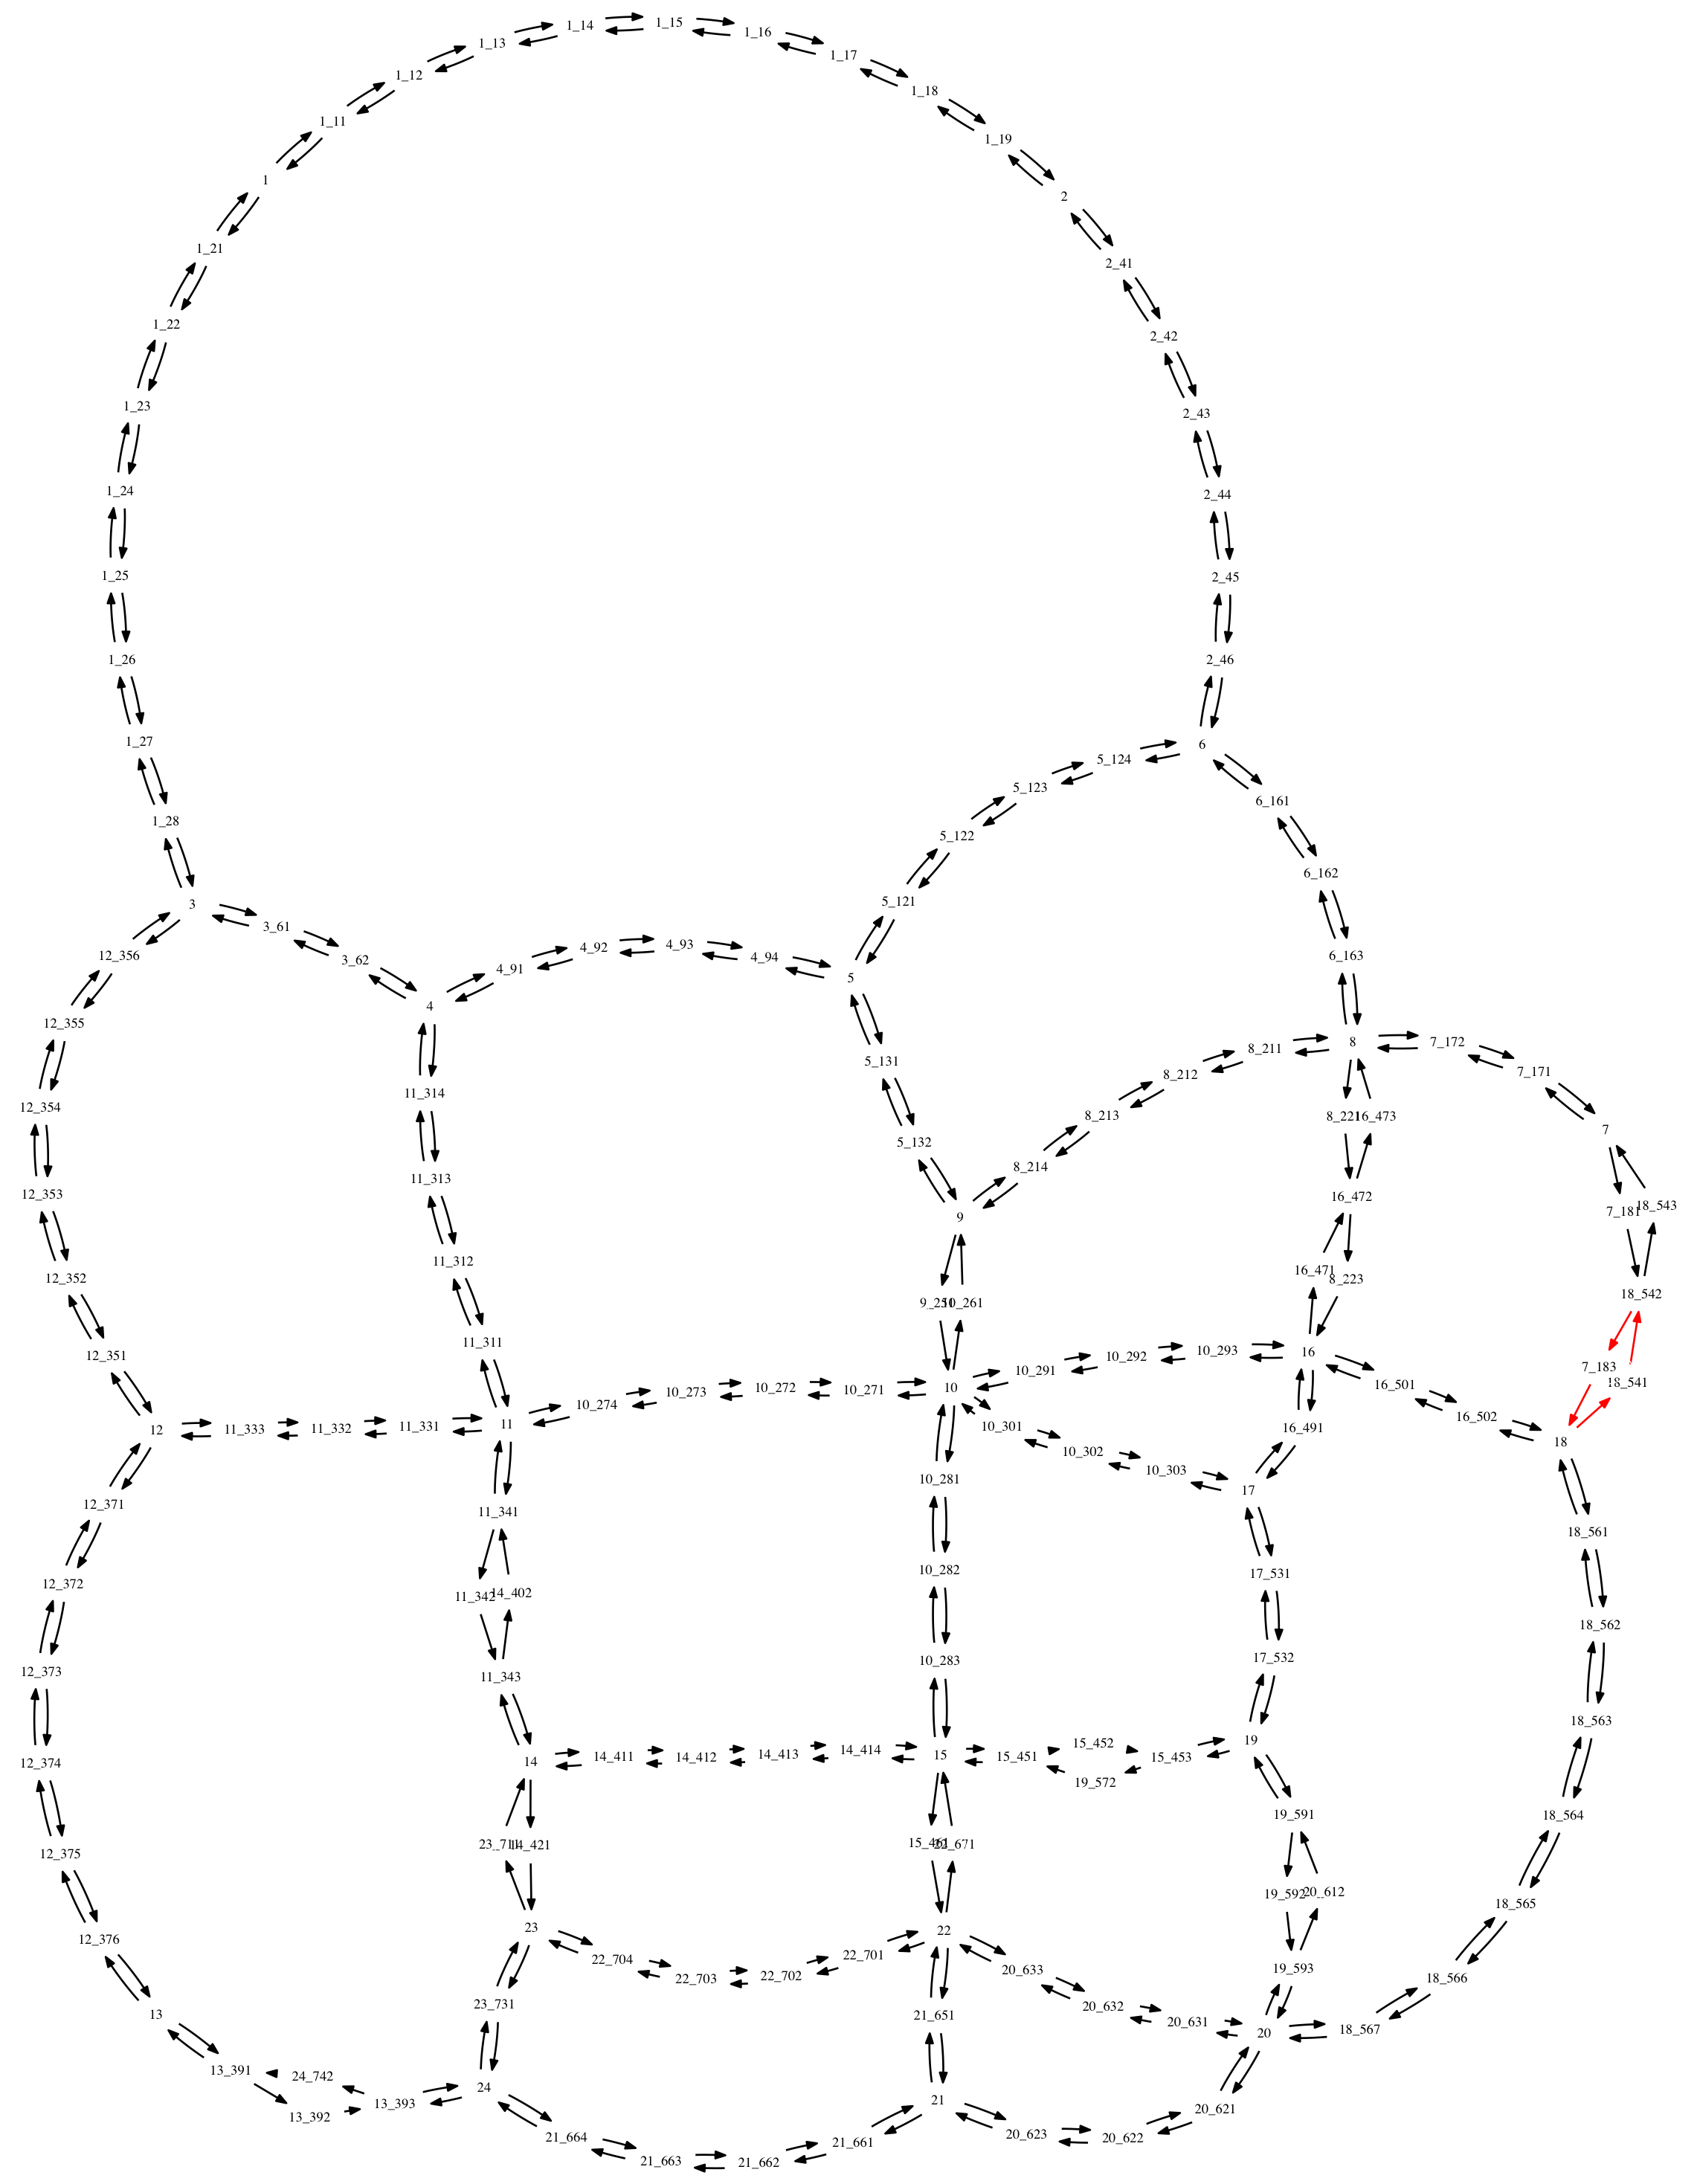
\includegraphics[totalheight=0.550\textheight, angle=90]{img/sioux-out/1/network2}};
	
	\draw[red,ultra thick] (7.7,9.5) rectangle (9.5,0 |- image.north);
%	\draw[red,ultra thick] (4.35,5.15) rectangle (6.75,8.0);
%	\draw[red,ultra thick] (10.4,5.5) rectangle (11.8,8.3);
%	\draw[red,ultra thick] (5.3,0) rectangle (9.6,1.6);
\end{tikzpicture}
\caption{Sieć miasta Sioux Falls, rozwiązanie nr 1}
\label{fig:sioux1}
\end{figure}

\begin{figure}[htbp]
\centering
\begin{tikzpicture}
    \node[anchor=south west] (image) at (0,0)
    {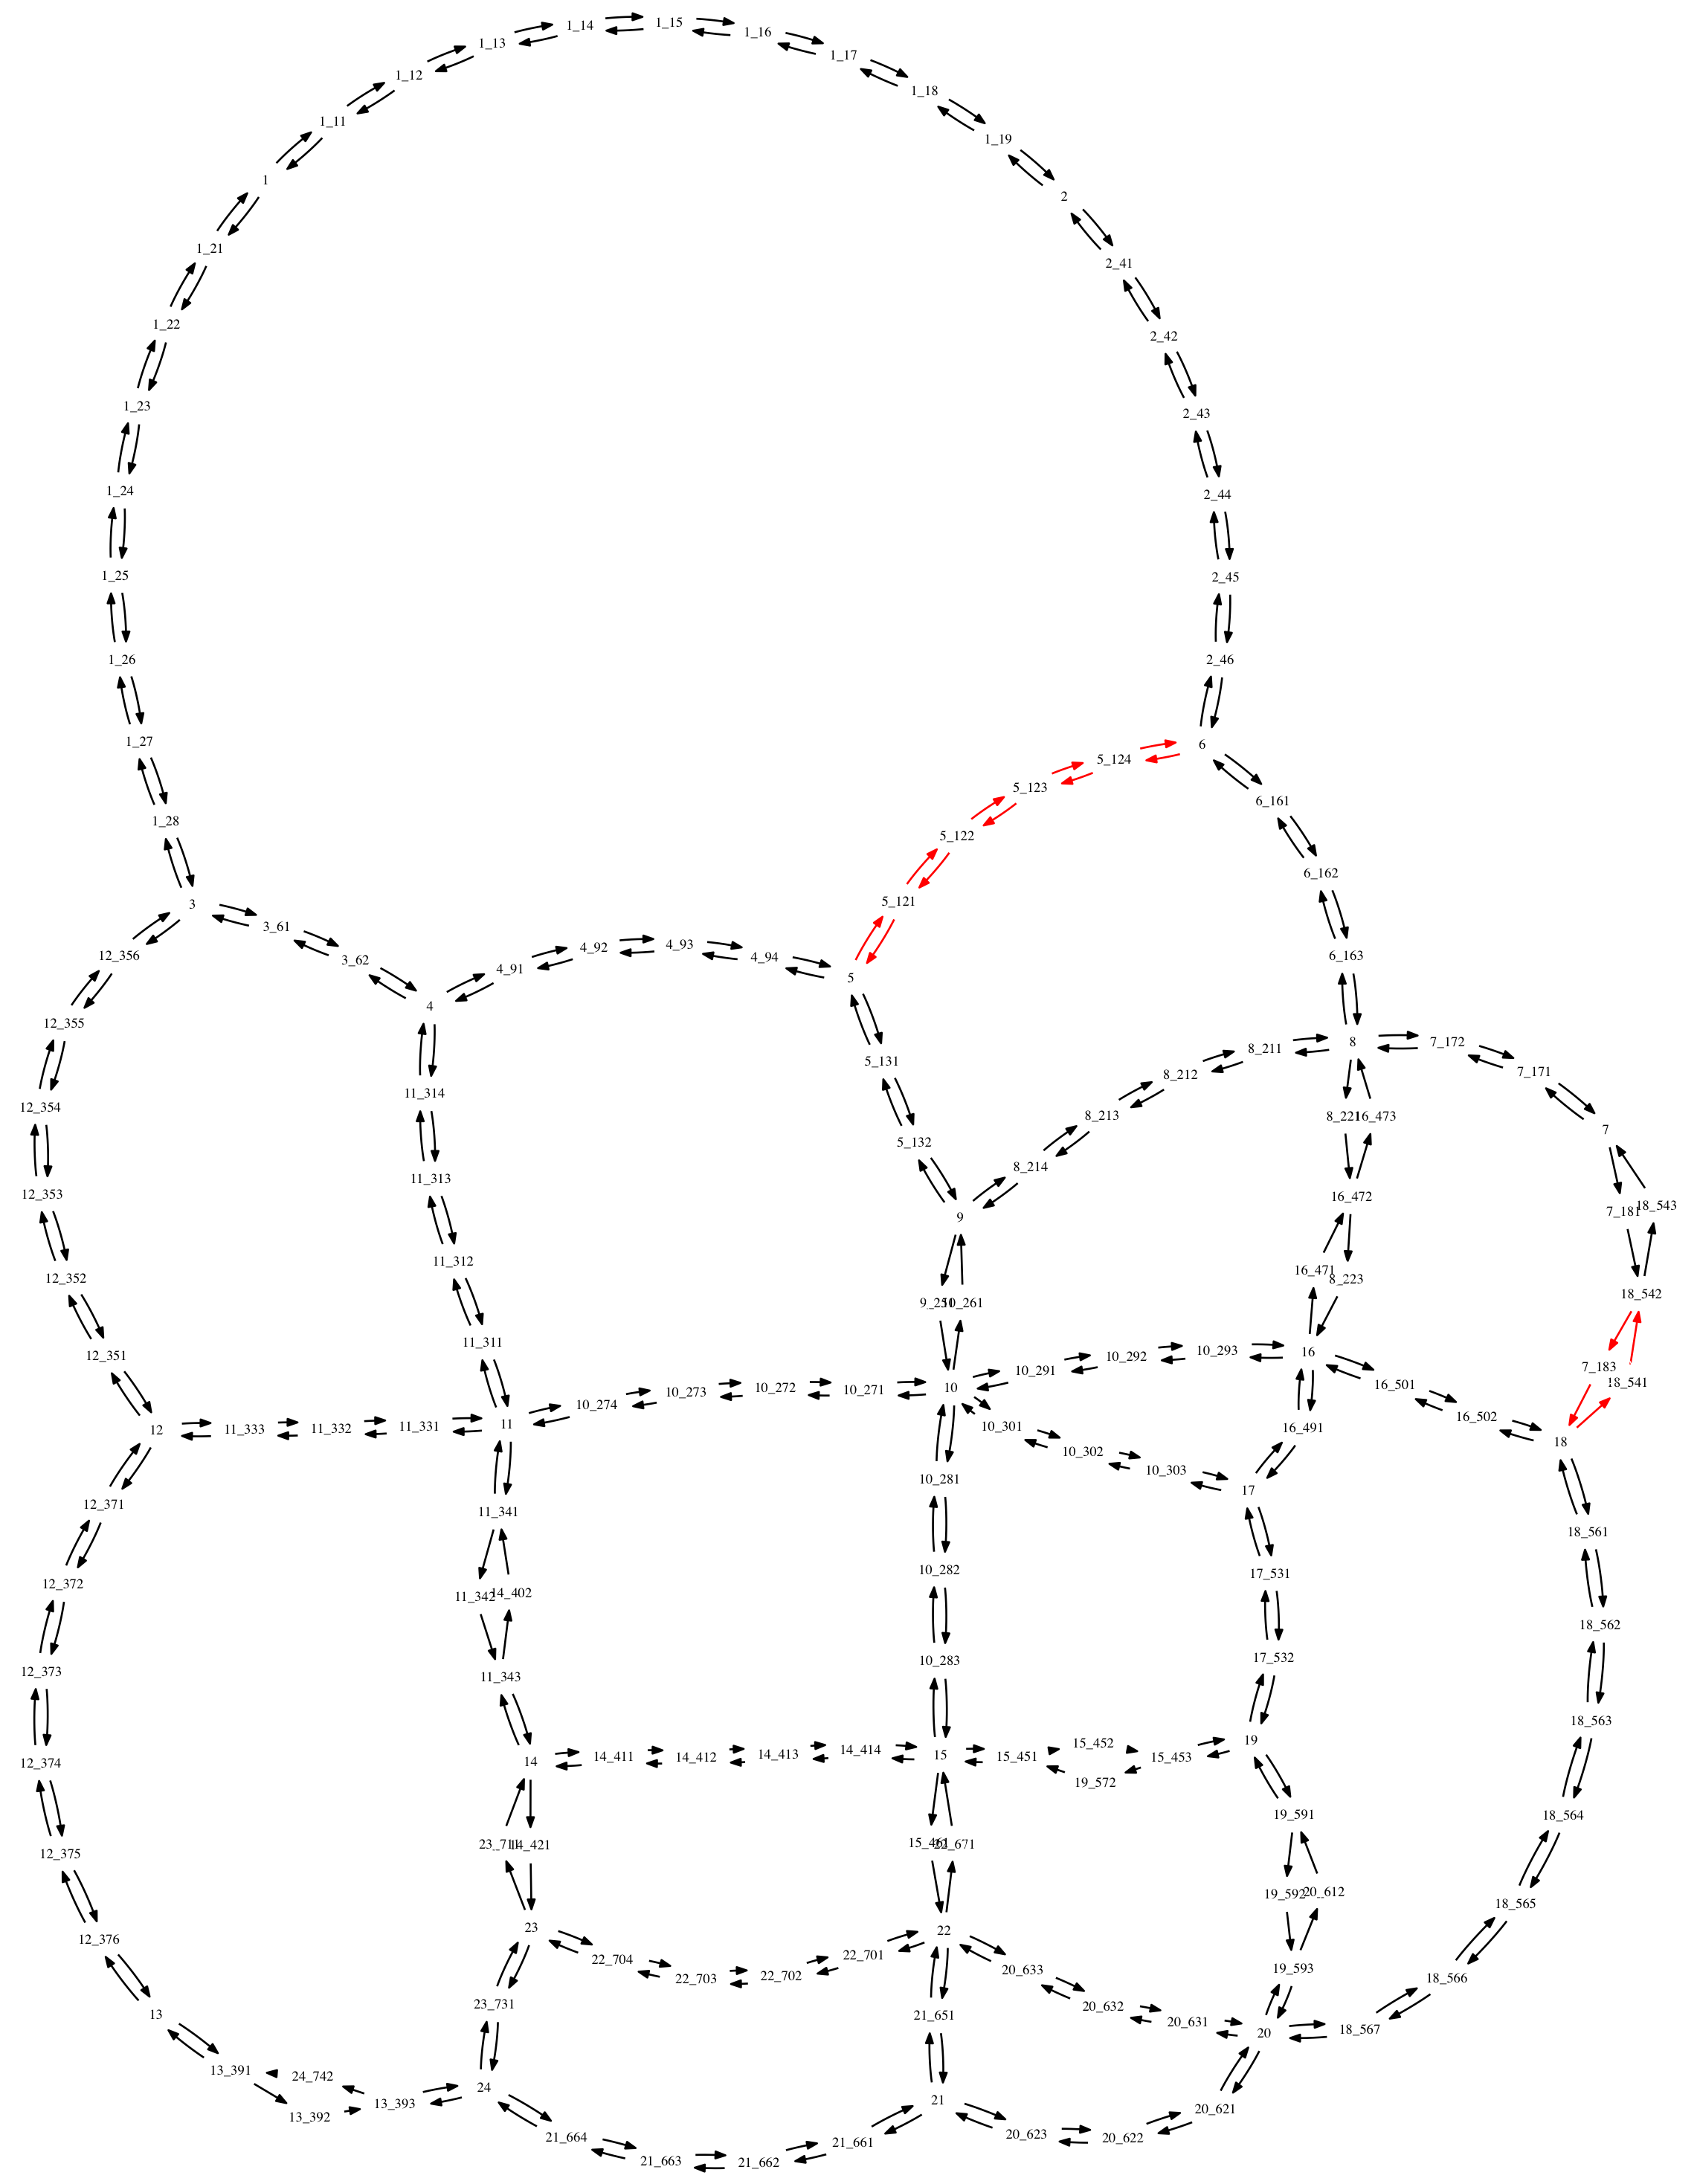
\includegraphics[totalheight=0.550\textheight, angle=90]{img/sioux-out/2/network2}};
	
	\draw[red,ultra thick] (7.7,9.5) rectangle (9.5,0 |- image.north);
	\draw[red,ultra thick] (4.35,5.15) rectangle (6.75,8.0);
%	\draw[red,ultra thick] (10.4,5.5) rectangle (11.8,8.3);
%	\draw[red,ultra thick] (5.3,0) rectangle (9.6,1.6);
\end{tikzpicture}
\caption{Sieć miasta Sioux Falls, rozwiązanie nr 2}
\label{fig:sioux2}
\end{figure}

\begin{figure}[htbp]
\centering
\begin{tikzpicture}
    \node[anchor=south west] (image) at (0,0)
    {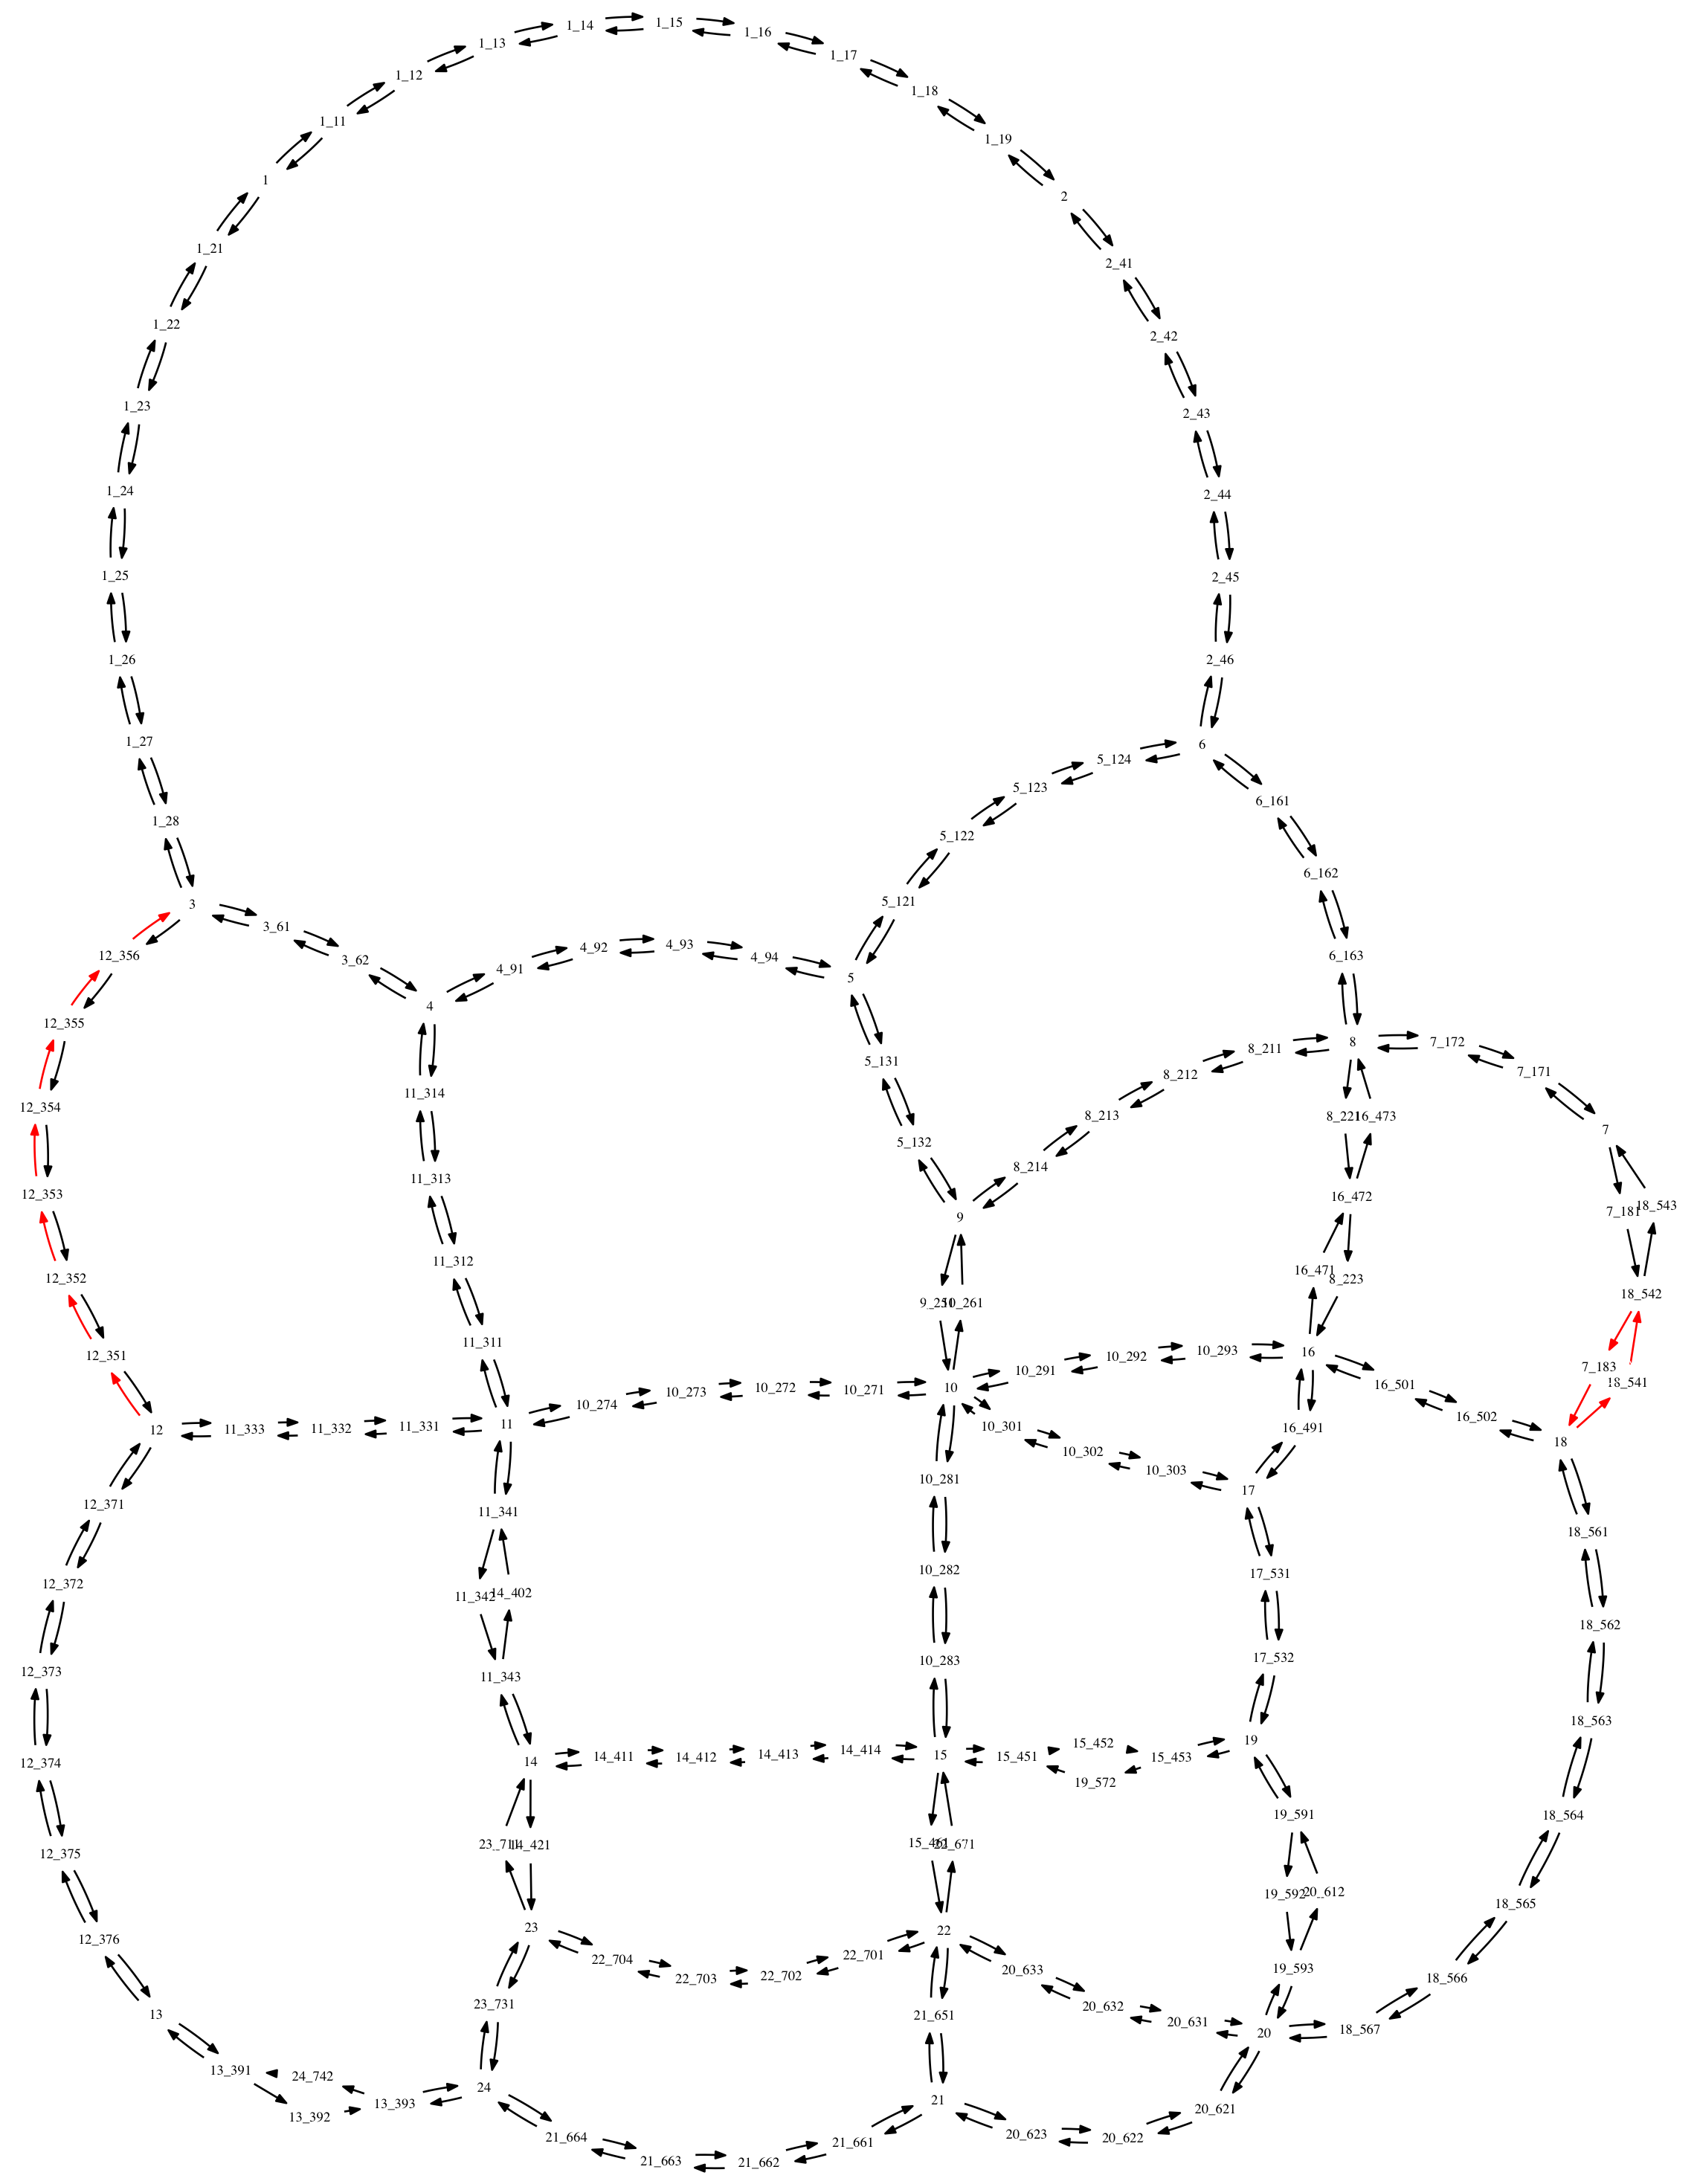
\includegraphics[totalheight=0.550\textheight, angle=90]{img/sioux-out/3/network2}};
	
	\draw[red,ultra thick] (7.7,9.5) rectangle (9.5,0 |- image.north);
%	\draw[red,ultra thick] (4.35,5.15) rectangle (6.75,8.0);
%	\draw[red,ultra thick] (10.4,5.5) rectangle (11.8,8.3);
	\draw[red,ultra thick] (5.3,0) rectangle (9.6,1.6);
\end{tikzpicture}
\caption{Sieć miasta Sioux Falls, rozwiązanie nr 3}
\label{fig:sioux3}
\end{figure}

\begin{figure}[htbp]
\centering
\begin{tikzpicture}
    \node[anchor=south west] (image) at (0,0)
    {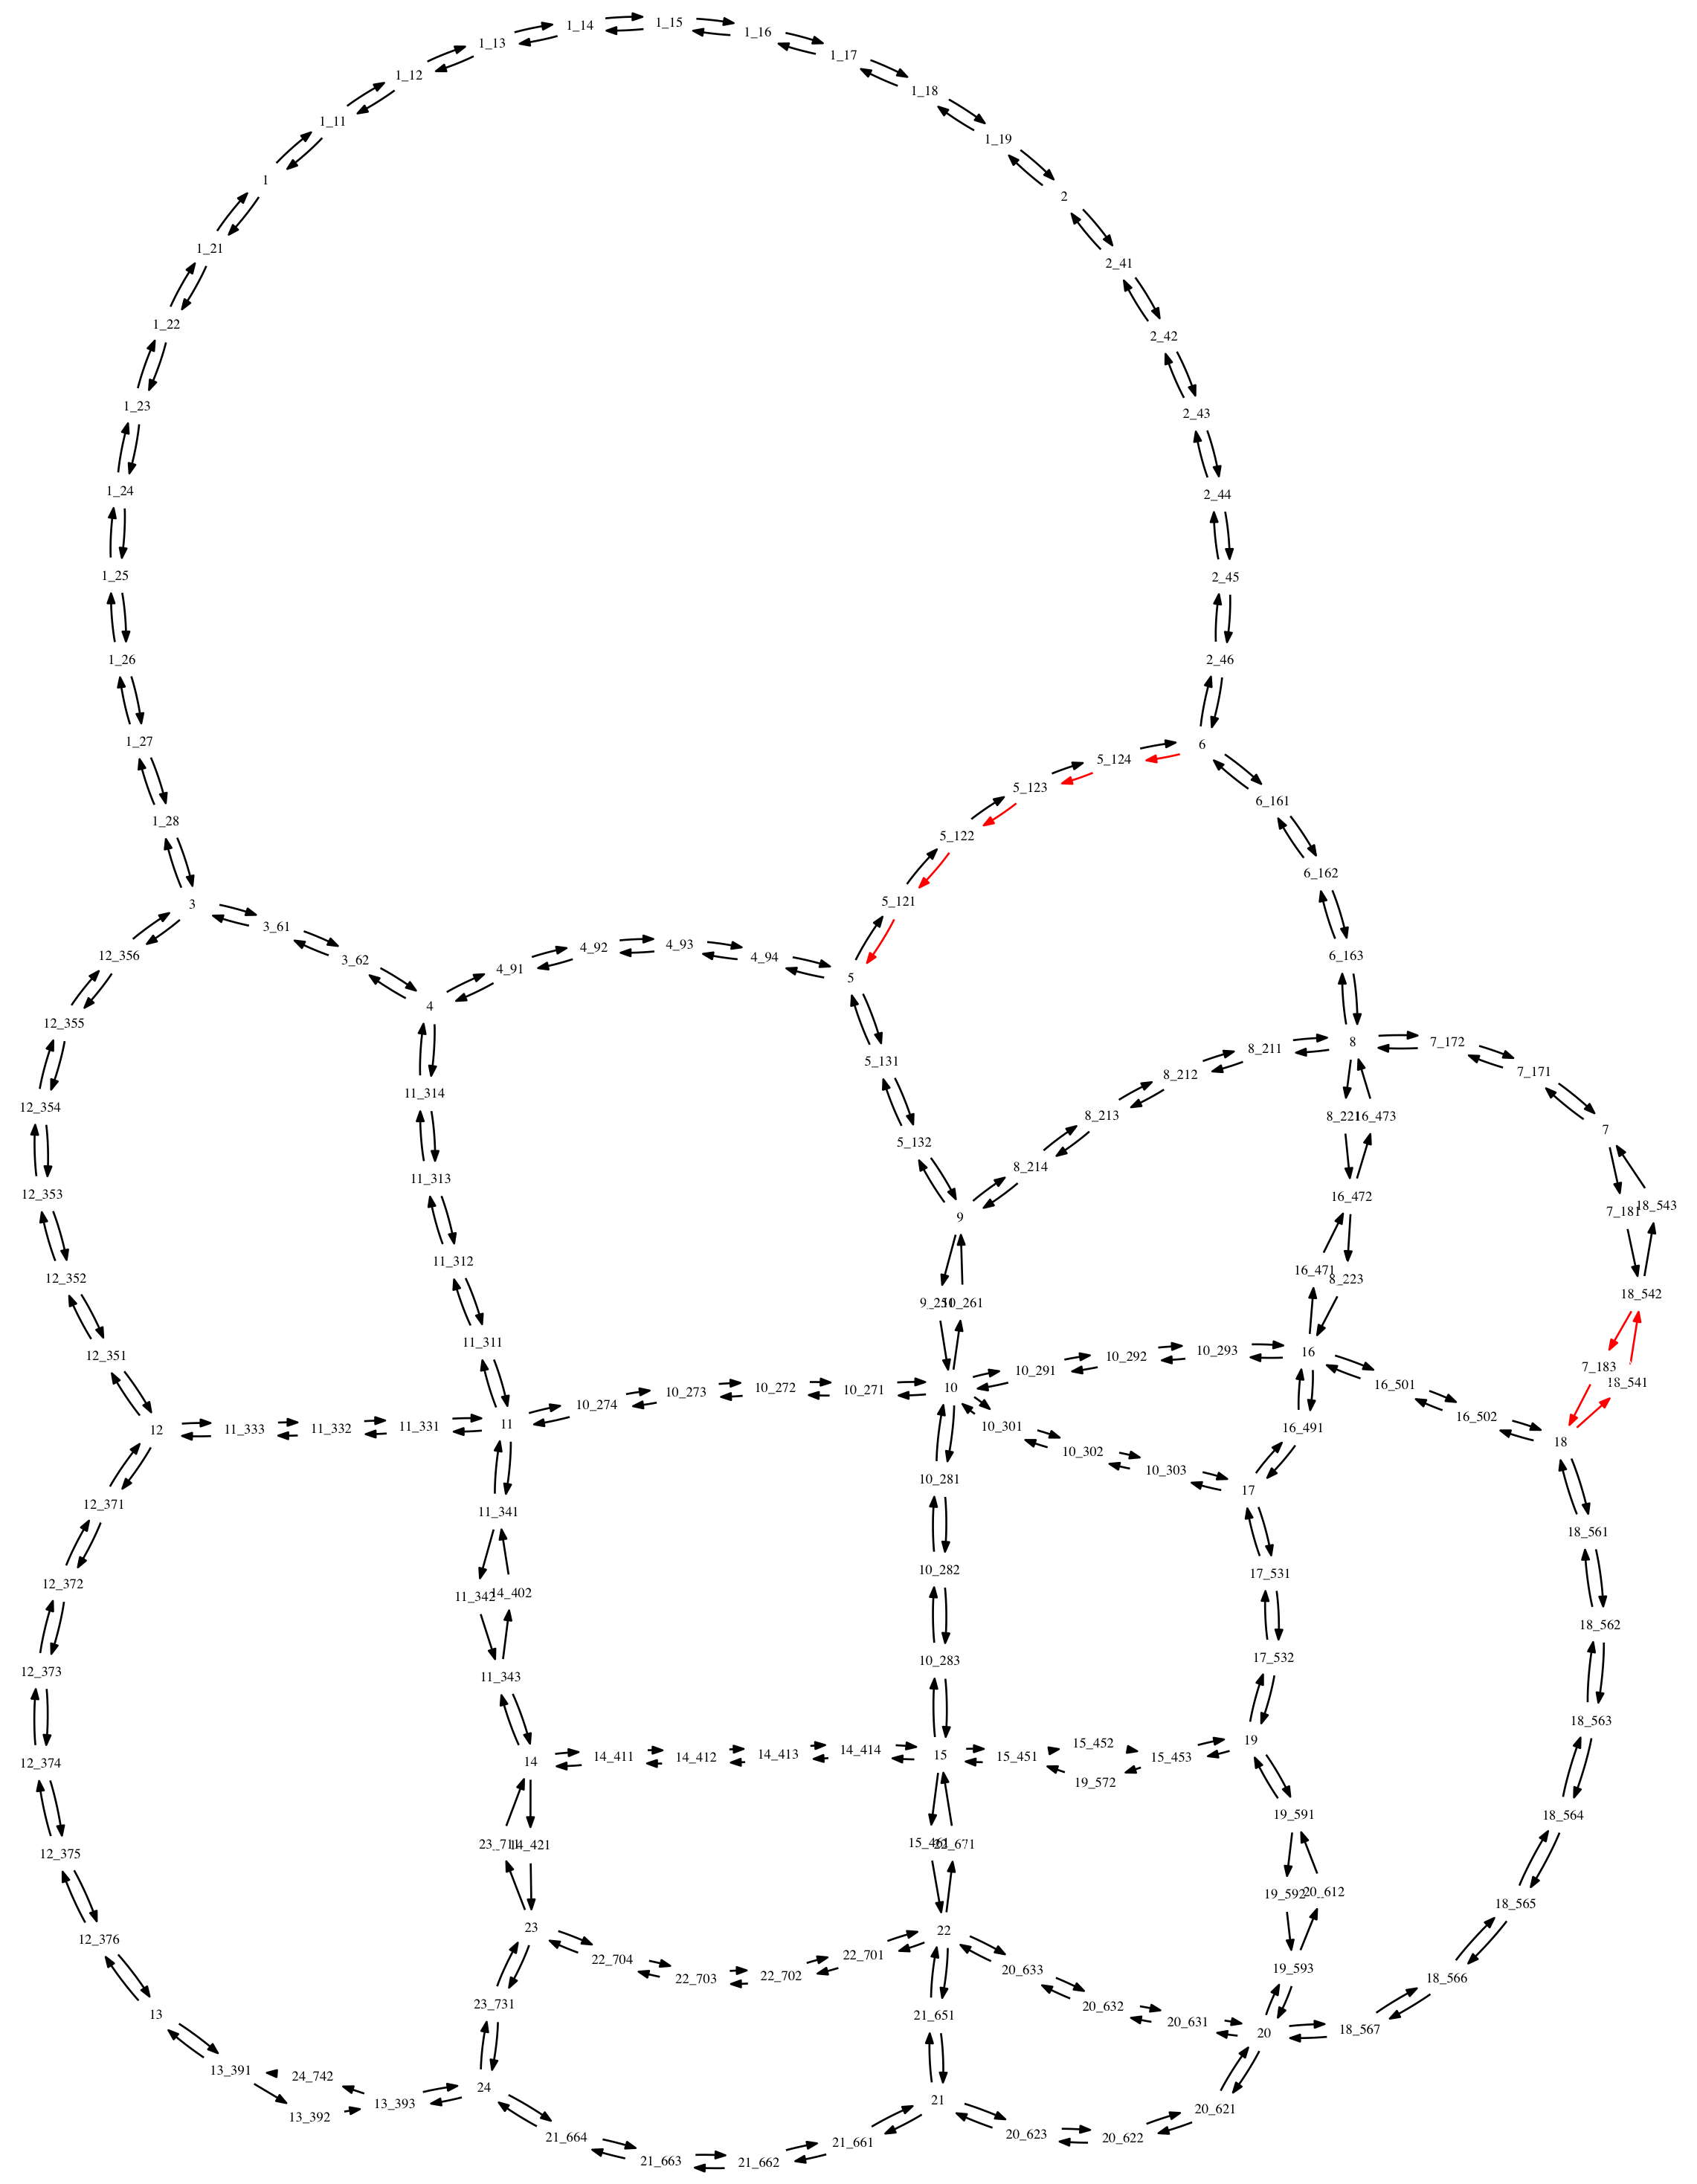
\includegraphics[totalheight=0.550\textheight, angle=90]{img/sioux-out/4/network2}};
	
	\draw[red,ultra thick] (7.7,9.5) rectangle (9.5,0 |- image.north);
	\draw[red,ultra thick] (4.35,5.15) rectangle (6.75,8.0);
%	\draw[red,ultra thick] (10.4,5.5) rectangle (11.8,8.3);
%	\draw[red,ultra thick] (5.3,0) rectangle (9.6,1.6);
\end{tikzpicture}
\caption{Sieć miasta Sioux Falls, rozwiązanie nr 4}
\label{fig:sioux4}
\end{figure}

\begin{figure}[htbp]
\centering
\begin{tikzpicture}
    \node[anchor=south west] (image) at (0,0)
    {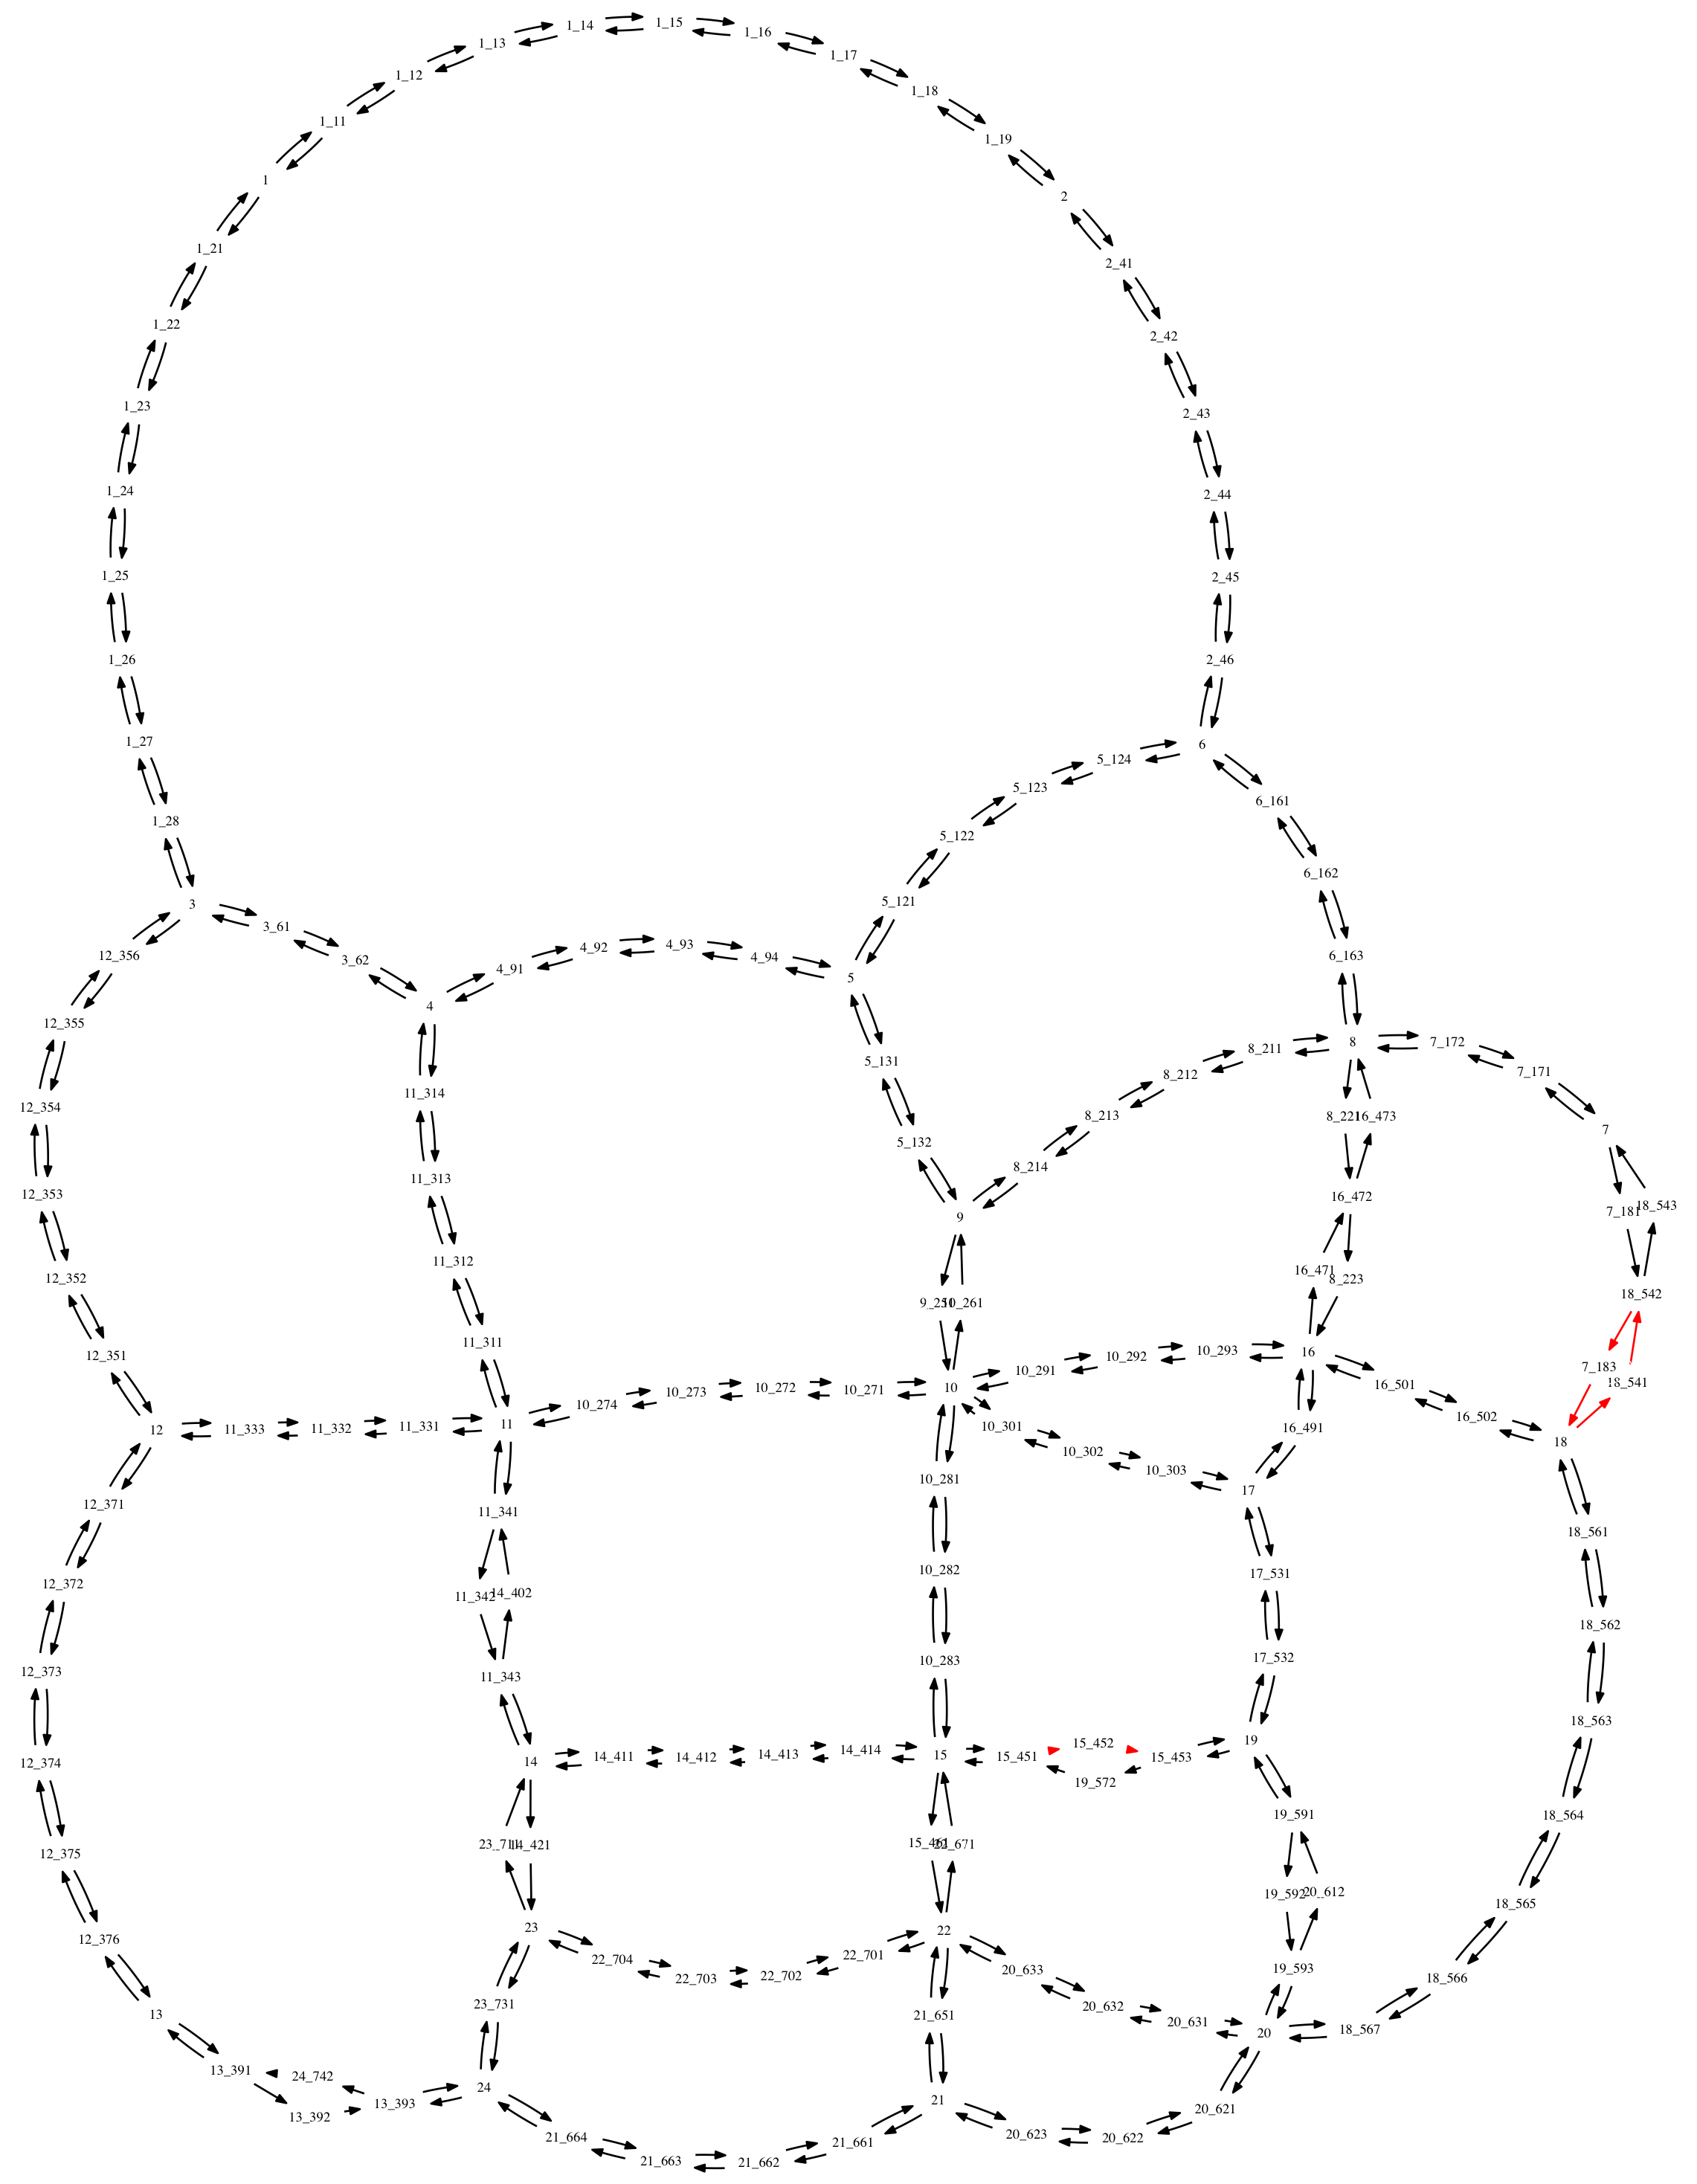
\includegraphics[totalheight=0.550\textheight, angle=90]{img/sioux-out/5/network2}};
	
	\draw[red,ultra thick] (7.7,9.5) rectangle (9.5,0 |- image.north);
%	\draw[red,ultra thick] (4.35,5.15) rectangle (6.75,8.0);
	\draw[red,ultra thick] (10.4,6.2) rectangle (11.8,7.6);
%	\draw[red,ultra thick] (5.3,0) rectangle (9.6,1.6);
\end{tikzpicture}
\caption{Sieć miasta Sioux Falls, rozwiązanie nr 5}
\label{fig:sioux5}
\end{figure}

\begin{figure}[htbp]
\centering
\begin{tikzpicture}
    \node[anchor=south west] (image) at (0,0)
    {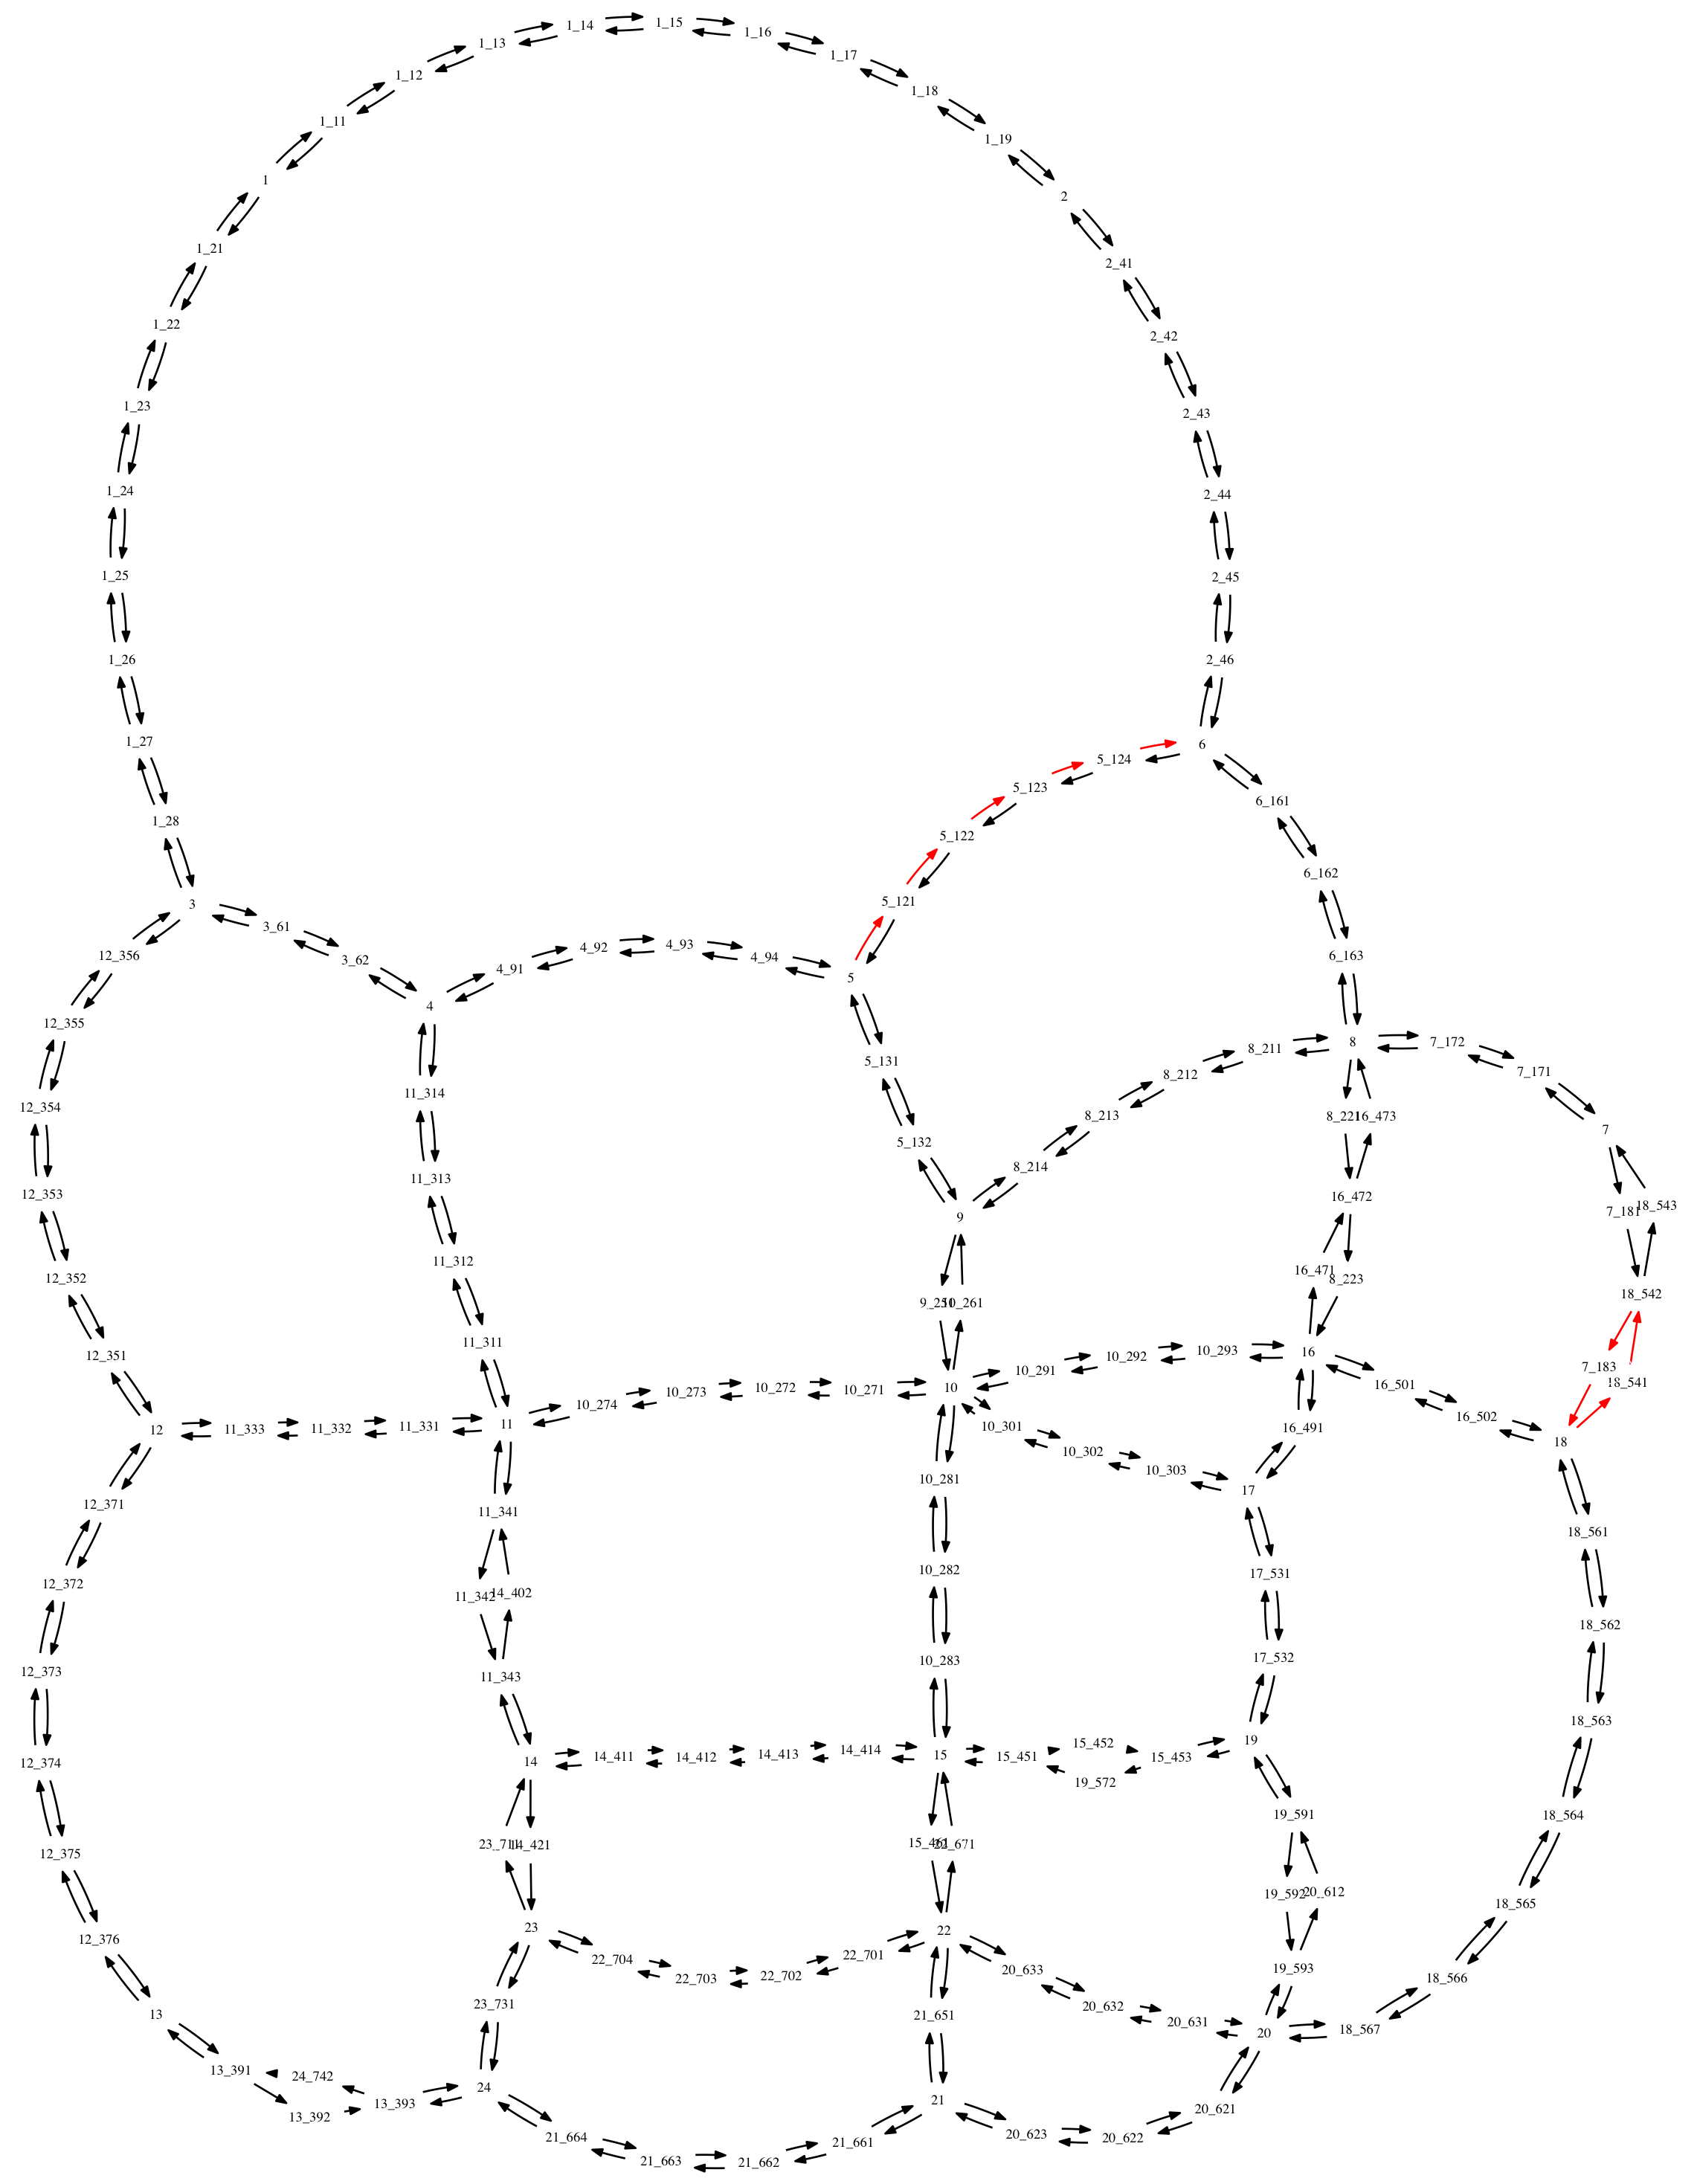
\includegraphics[totalheight=0.550\textheight, angle=90]{img/sioux-out/6/network2}};
	
	\draw[red,ultra thick] (7.7,9.5) rectangle (9.5,0 |- image.north);
	\draw[red,ultra thick] (4.35,5.15) rectangle (6.75,8.0);
%	\draw[red,ultra thick] (10.4,5.5) rectangle (11.8,8.3);
%	\draw[red,ultra thick] (5.3,0) rectangle (9.6,1.6);
\end{tikzpicture}
\caption{Sieć miasta Sioux Falls, rozwiązanie nr 6}
\label{fig:sioux6}
\end{figure}

\begin{figure}[htbp]
\centering
\begin{tikzpicture}
    \node[anchor=south west] (image) at (0,0)
    {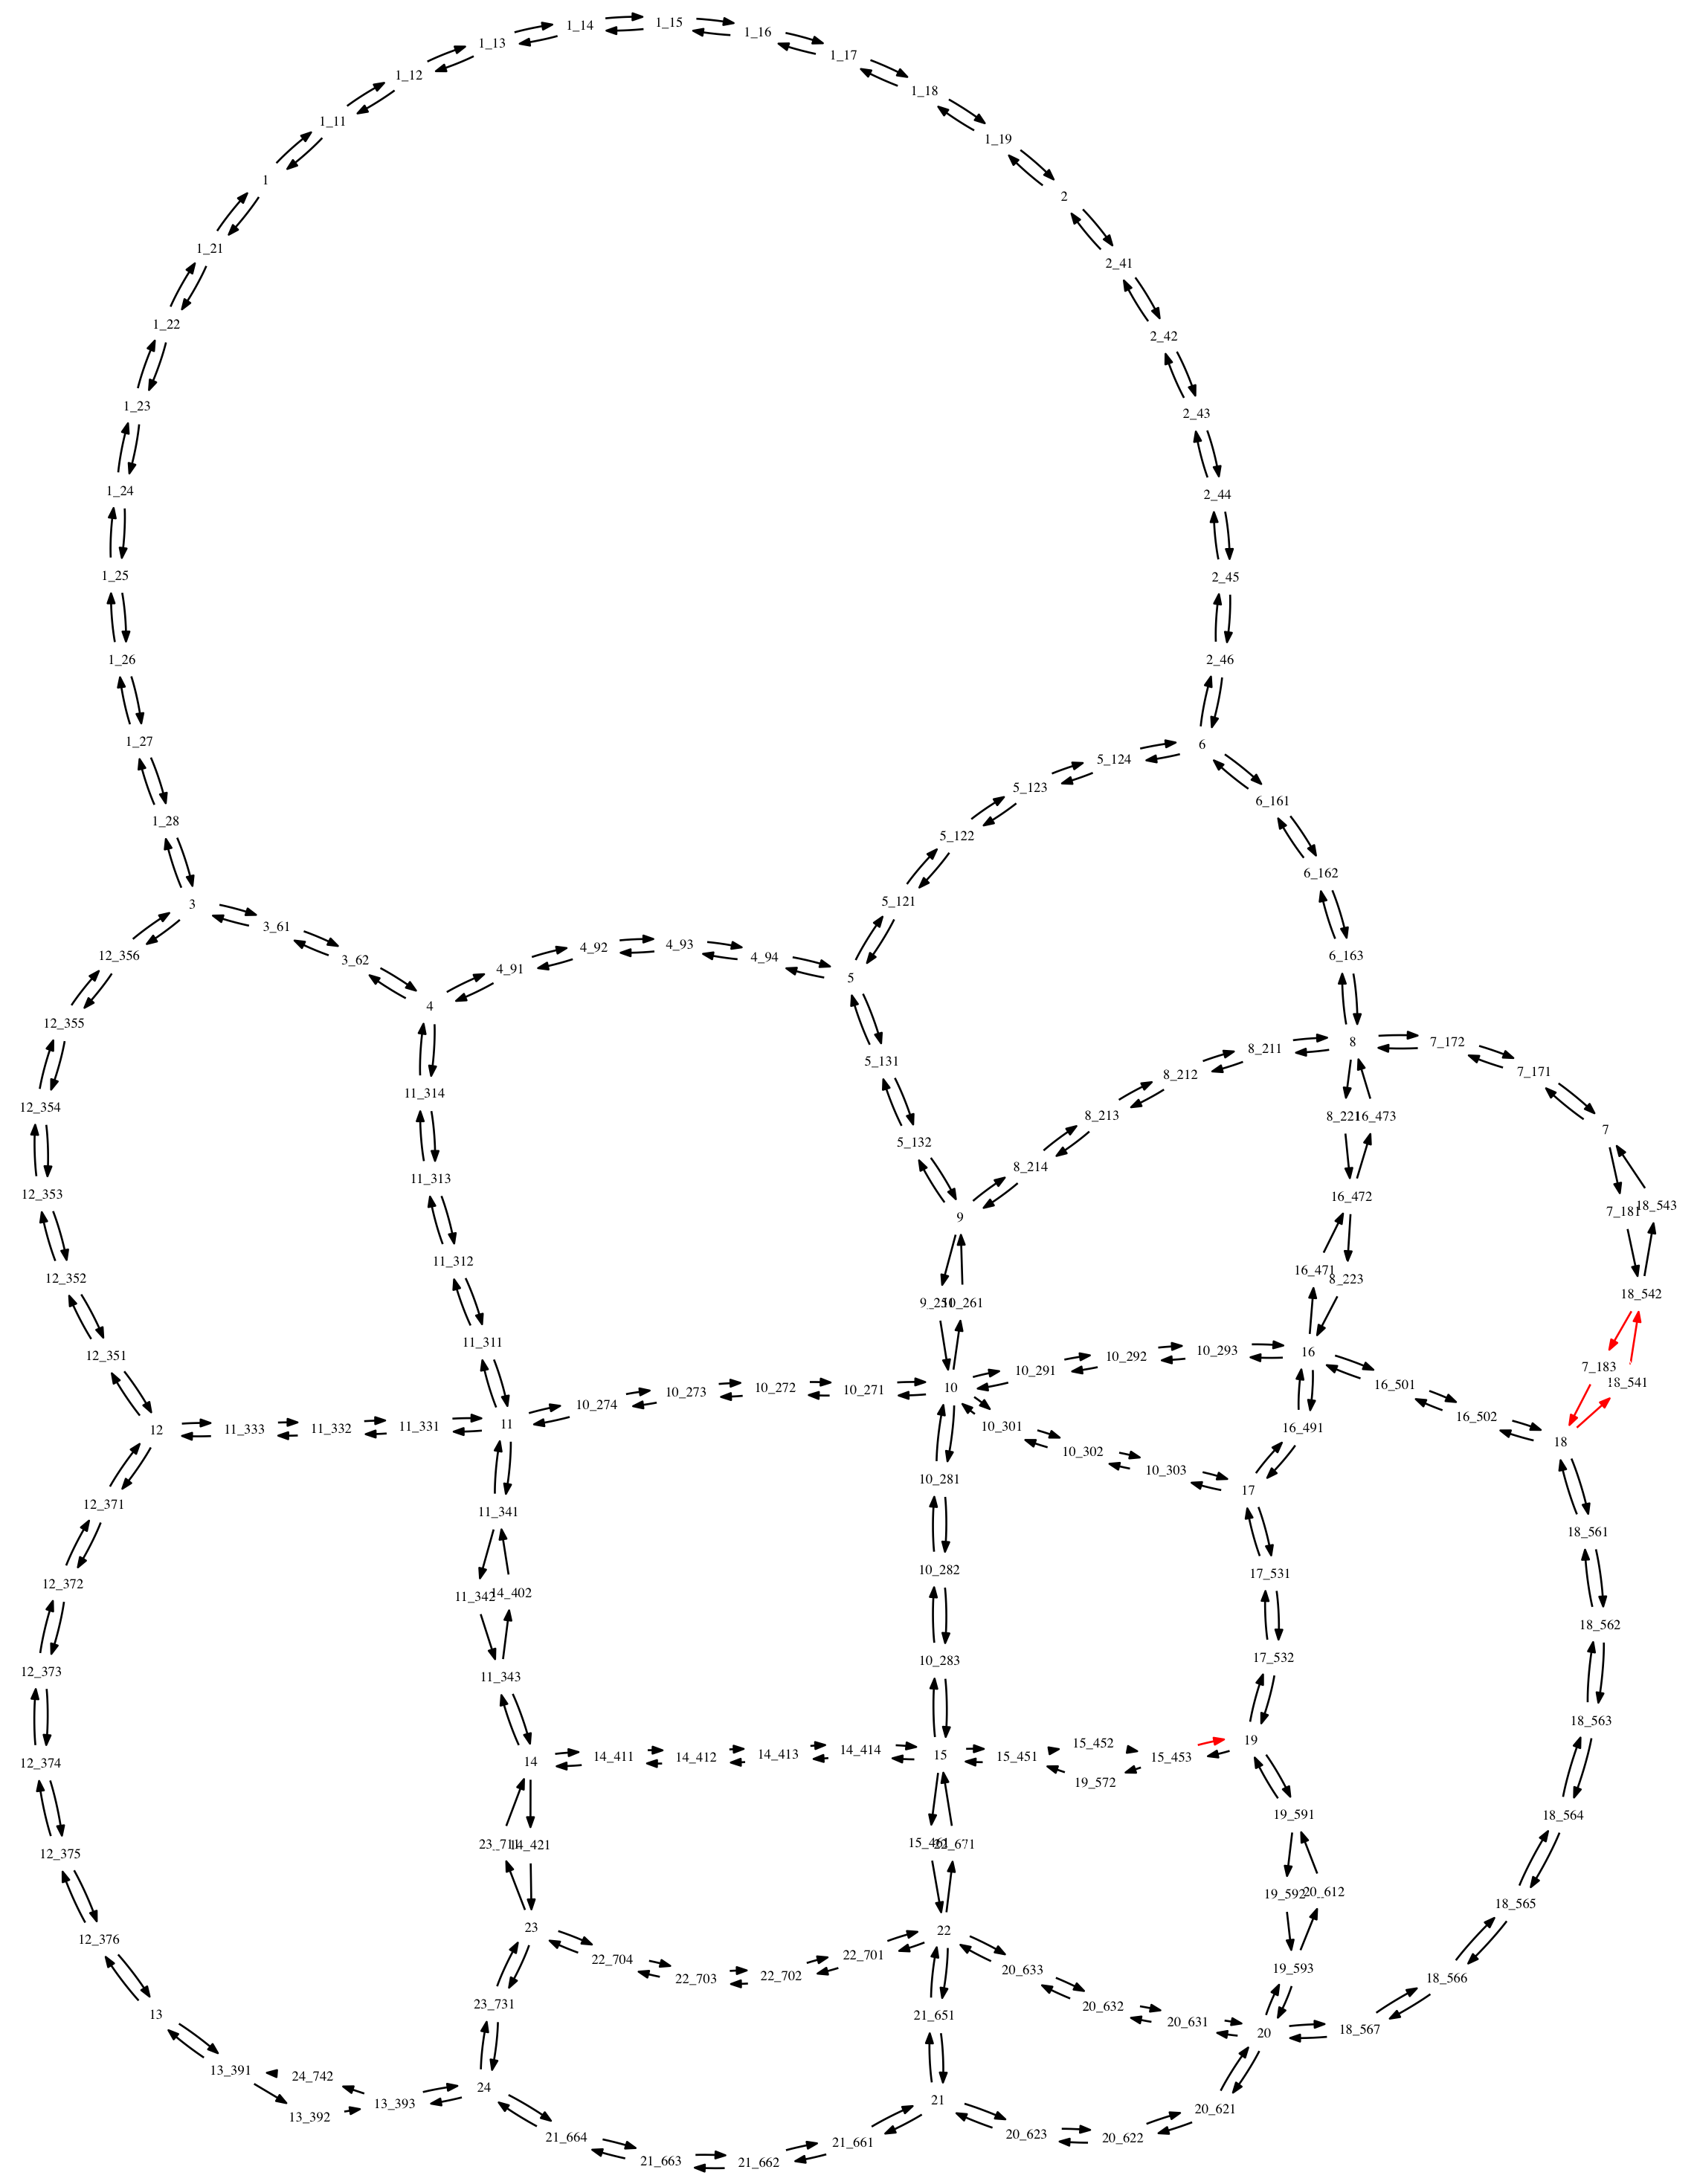
\includegraphics[totalheight=0.550\textheight, angle=90]{img/sioux-out/7/network2}};
	
	\draw[red,ultra thick] (7.7,9.5) rectangle (9.5,0 |- image.north);
%	\draw[red,ultra thick] (4.35,5.15) rectangle (6.75,8.0);
	\draw[red,ultra thick] (10.6,7.2) rectangle (11.5,8.2);
%	\draw[red,ultra thick] (5.3,0) rectangle (9.6,1.6);
\end{tikzpicture}
\caption{Sieć miasta Sioux Falls, rozwiązanie nr 7}
\label{fig:sioux7}
\end{figure}

\begin{figure}[htbp]
\centering
\begin{tikzpicture}
    \node[anchor=south west] (image) at (0,0)
    {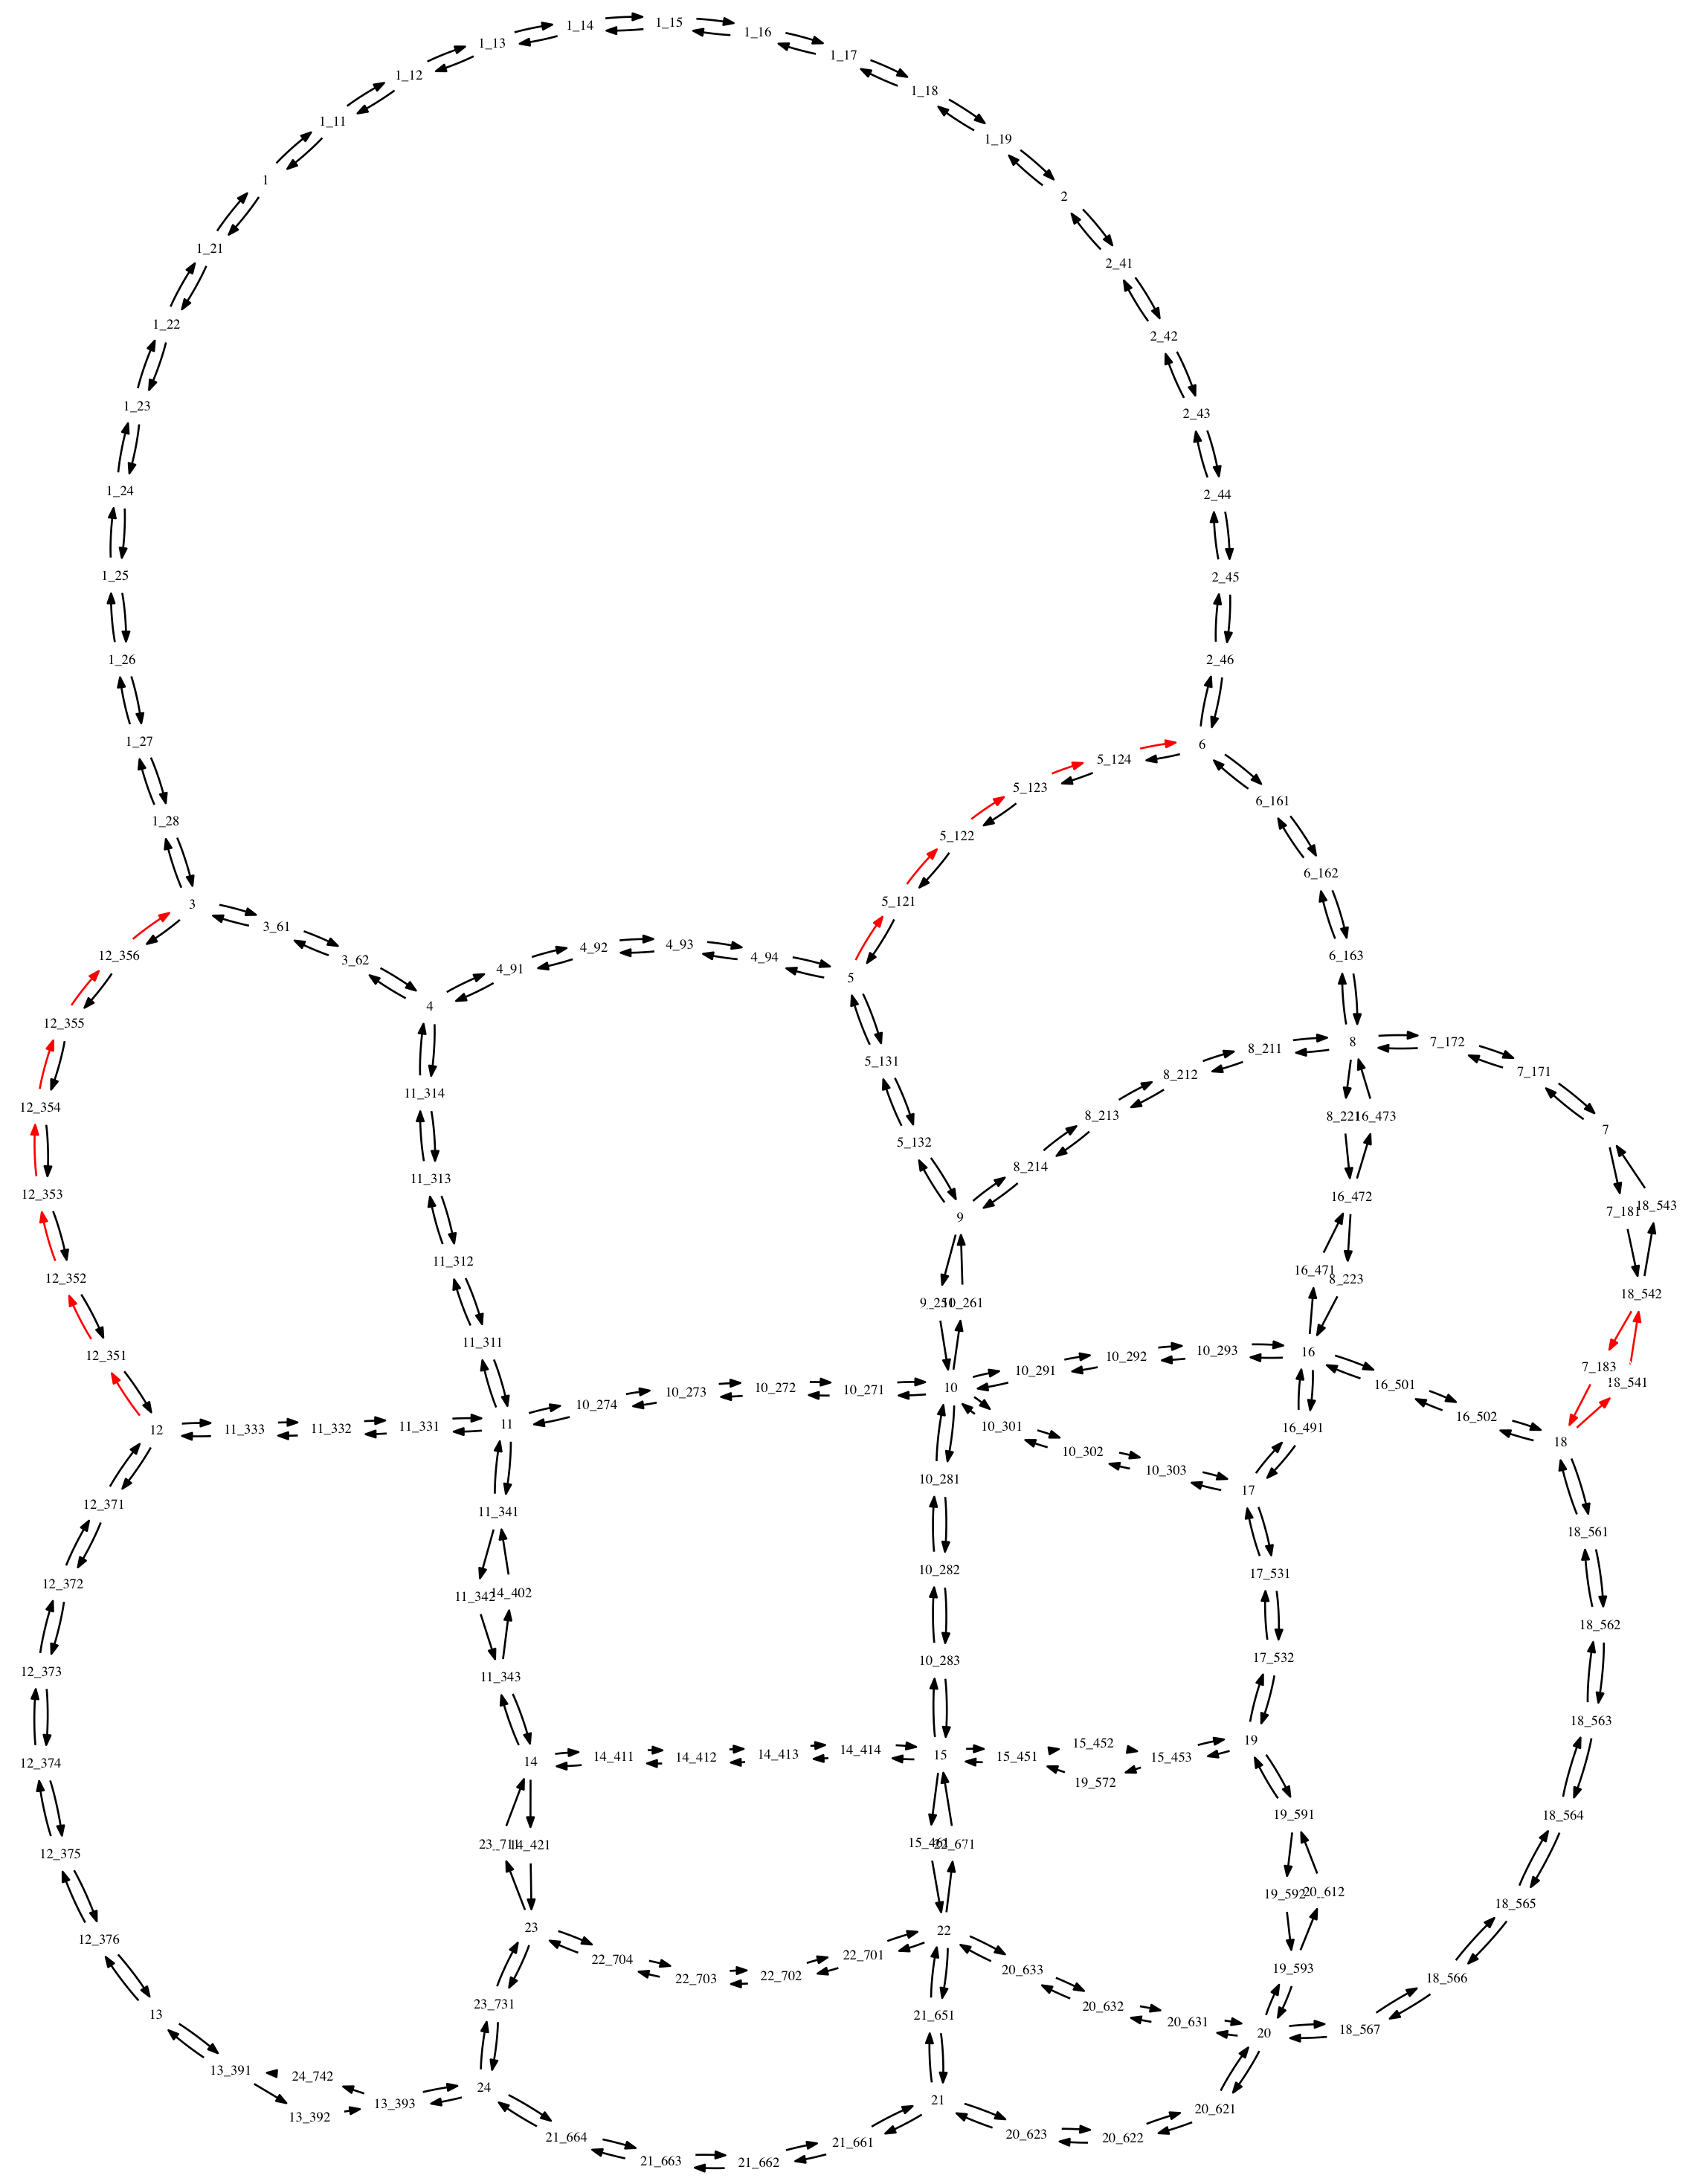
\includegraphics[totalheight=0.550\textheight, angle=90]{img/sioux-out/8/network2}};
	
	\draw[red,ultra thick] (7.7,9.5) rectangle (9.5,0 |- image.north);
	\draw[red,ultra thick] (4.35,5.15) rectangle (6.75,8.0);
%	\draw[red,ultra thick] (10.4,5.5) rectangle (11.8,8.3);
	\draw[red,ultra thick] (5.3,0) rectangle (9.6,1.6);
\end{tikzpicture}
\caption{Sieć miasta Sioux Falls, rozwiązanie nr 8}
\label{fig:sioux8}
\end{figure}

\begin{figure}[htbp]
\centering
\begin{tikzpicture}
    \node[anchor=south west] (image) at (0,0)
    {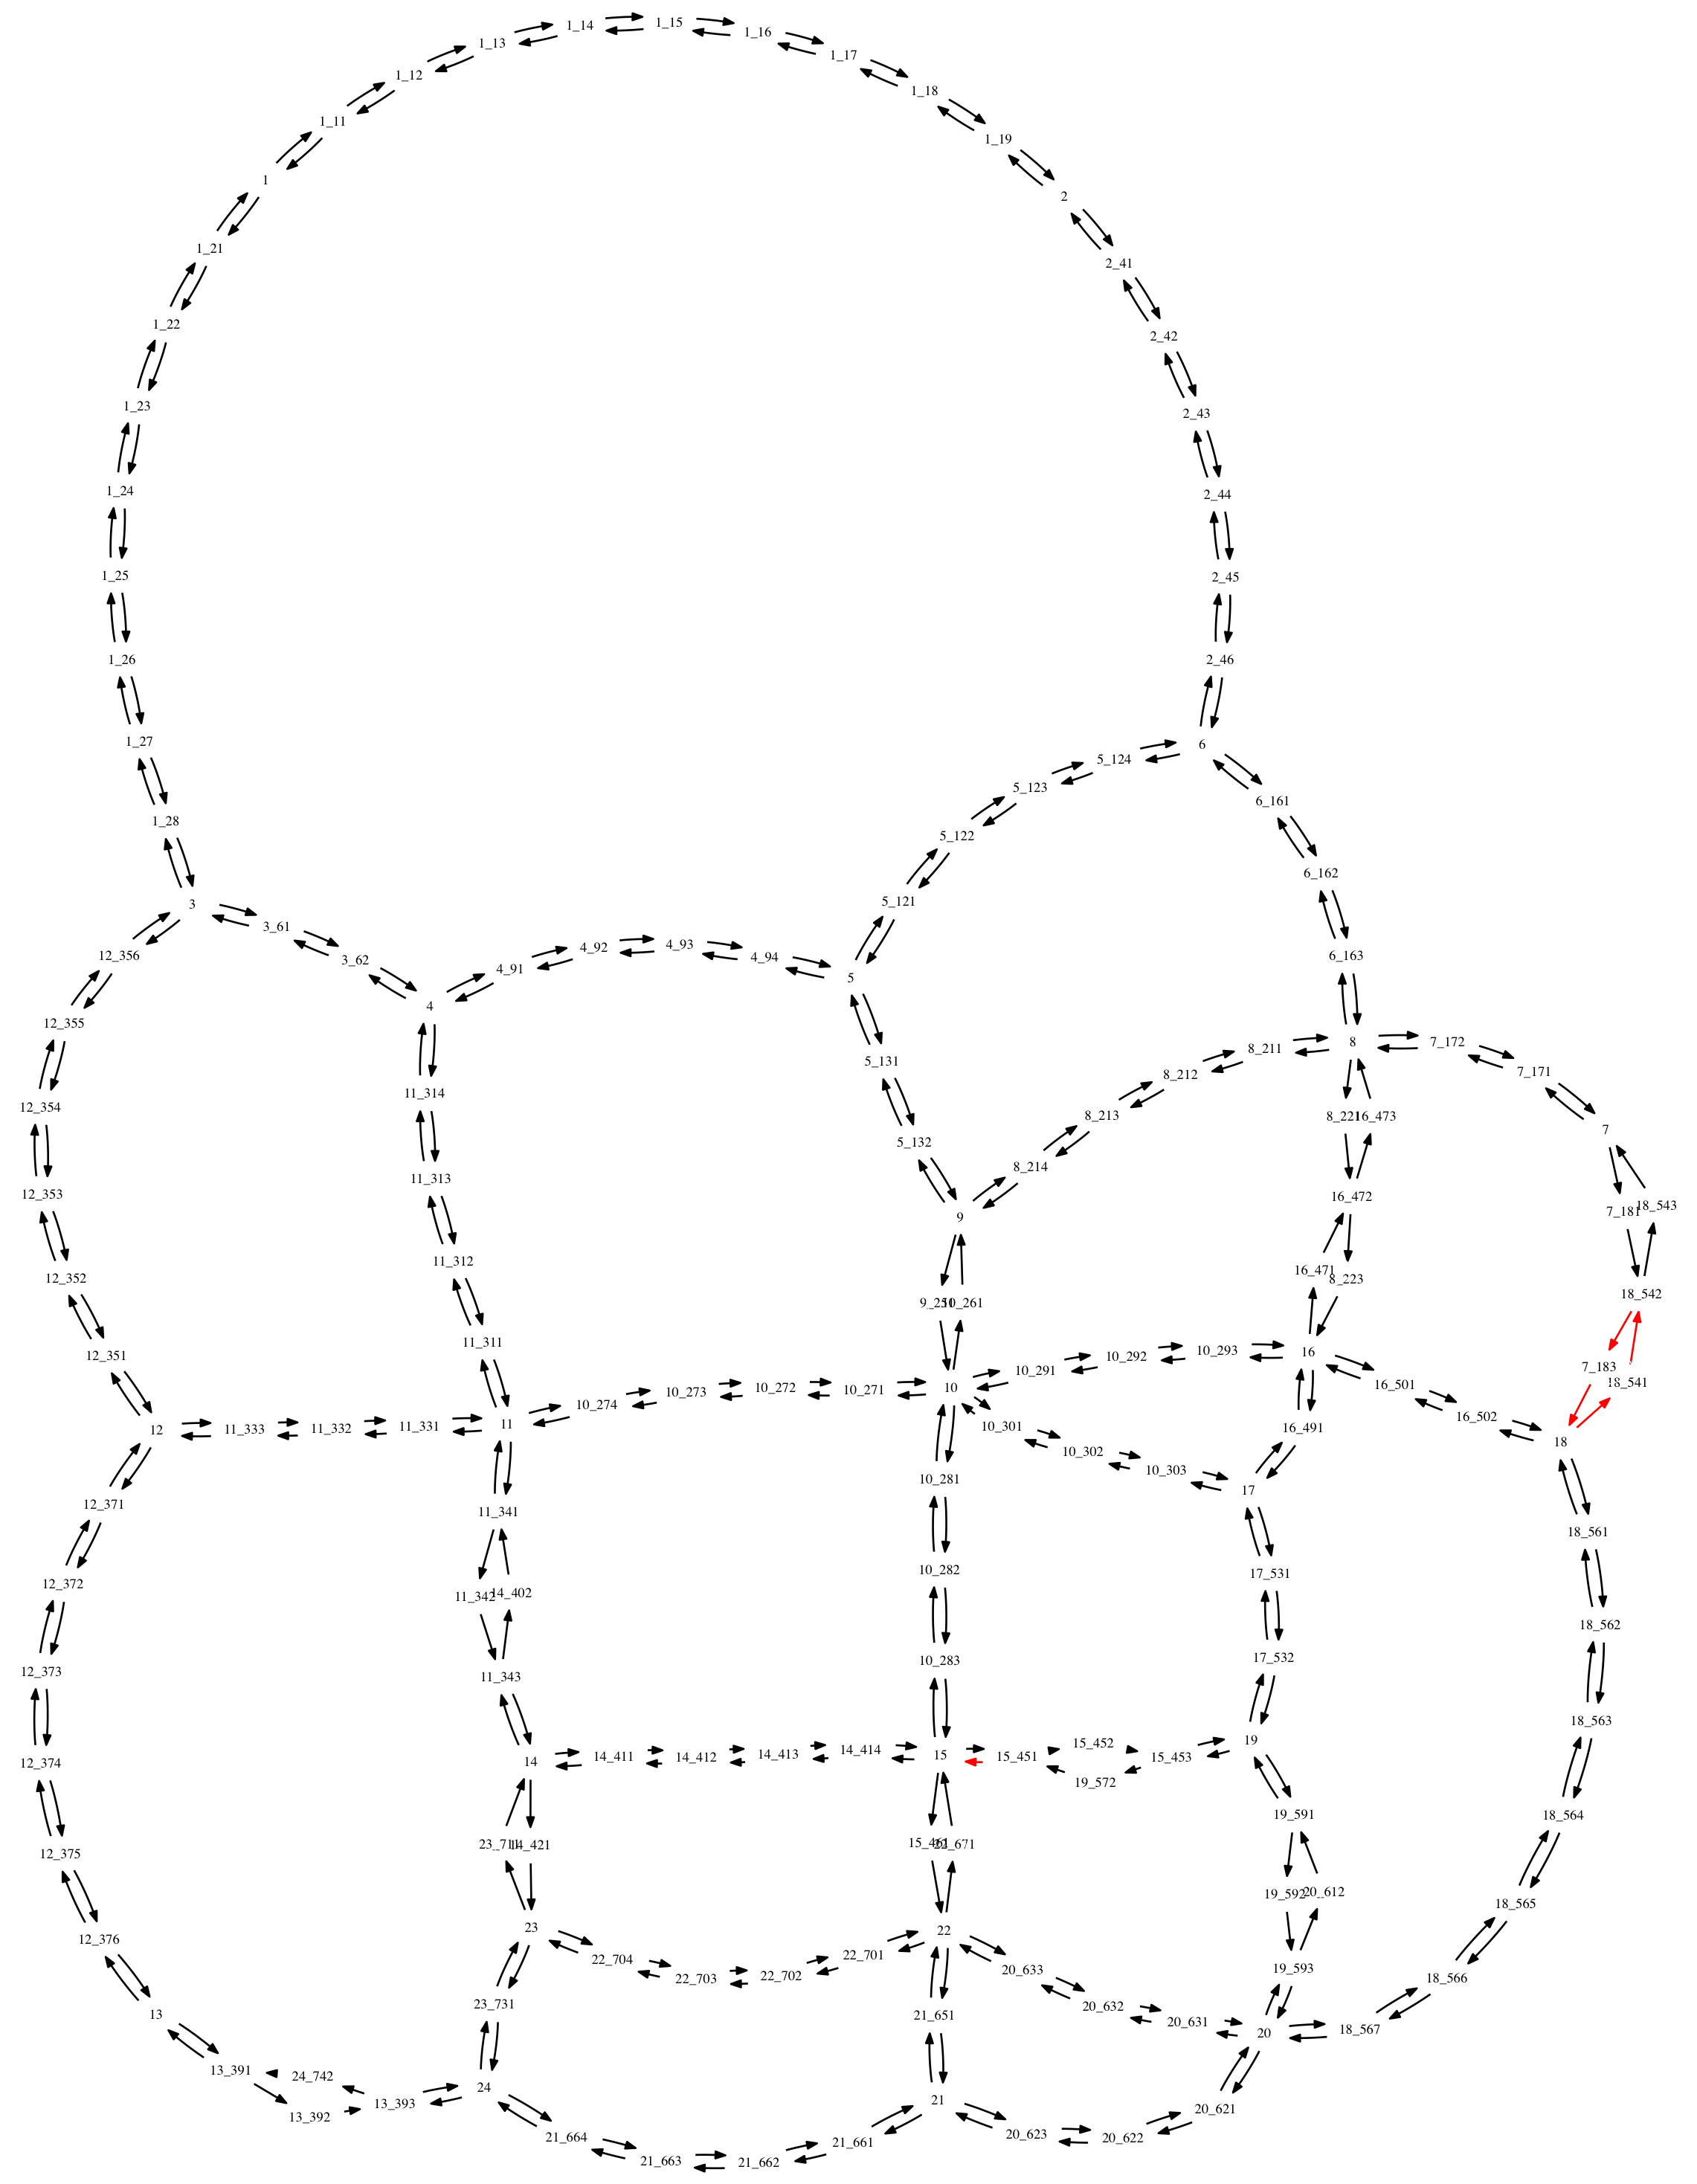
\includegraphics[totalheight=0.550\textheight, angle=90]{img/sioux-out/9/network2}};
	
	\draw[red,ultra thick] (7.7,9.5) rectangle (9.5,0 |- image.north);
%	\draw[red,ultra thick] (4.35,5.15) rectangle (6.75,8.0);
	\draw[red,ultra thick] (10.7,5.7) rectangle (11.5,6.7);
%	\draw[red,ultra thick] (5.3,0) rectangle (9.6,1.6);
\end{tikzpicture}
\caption{Sieć miasta Sioux Falls, rozwiązanie nr 9}
\label{fig:sioux9}
\end{figure}

\begin{figure}[htbp]
\centering
\begin{tikzpicture}
    \node[anchor=south west] (image) at (0,0)
    {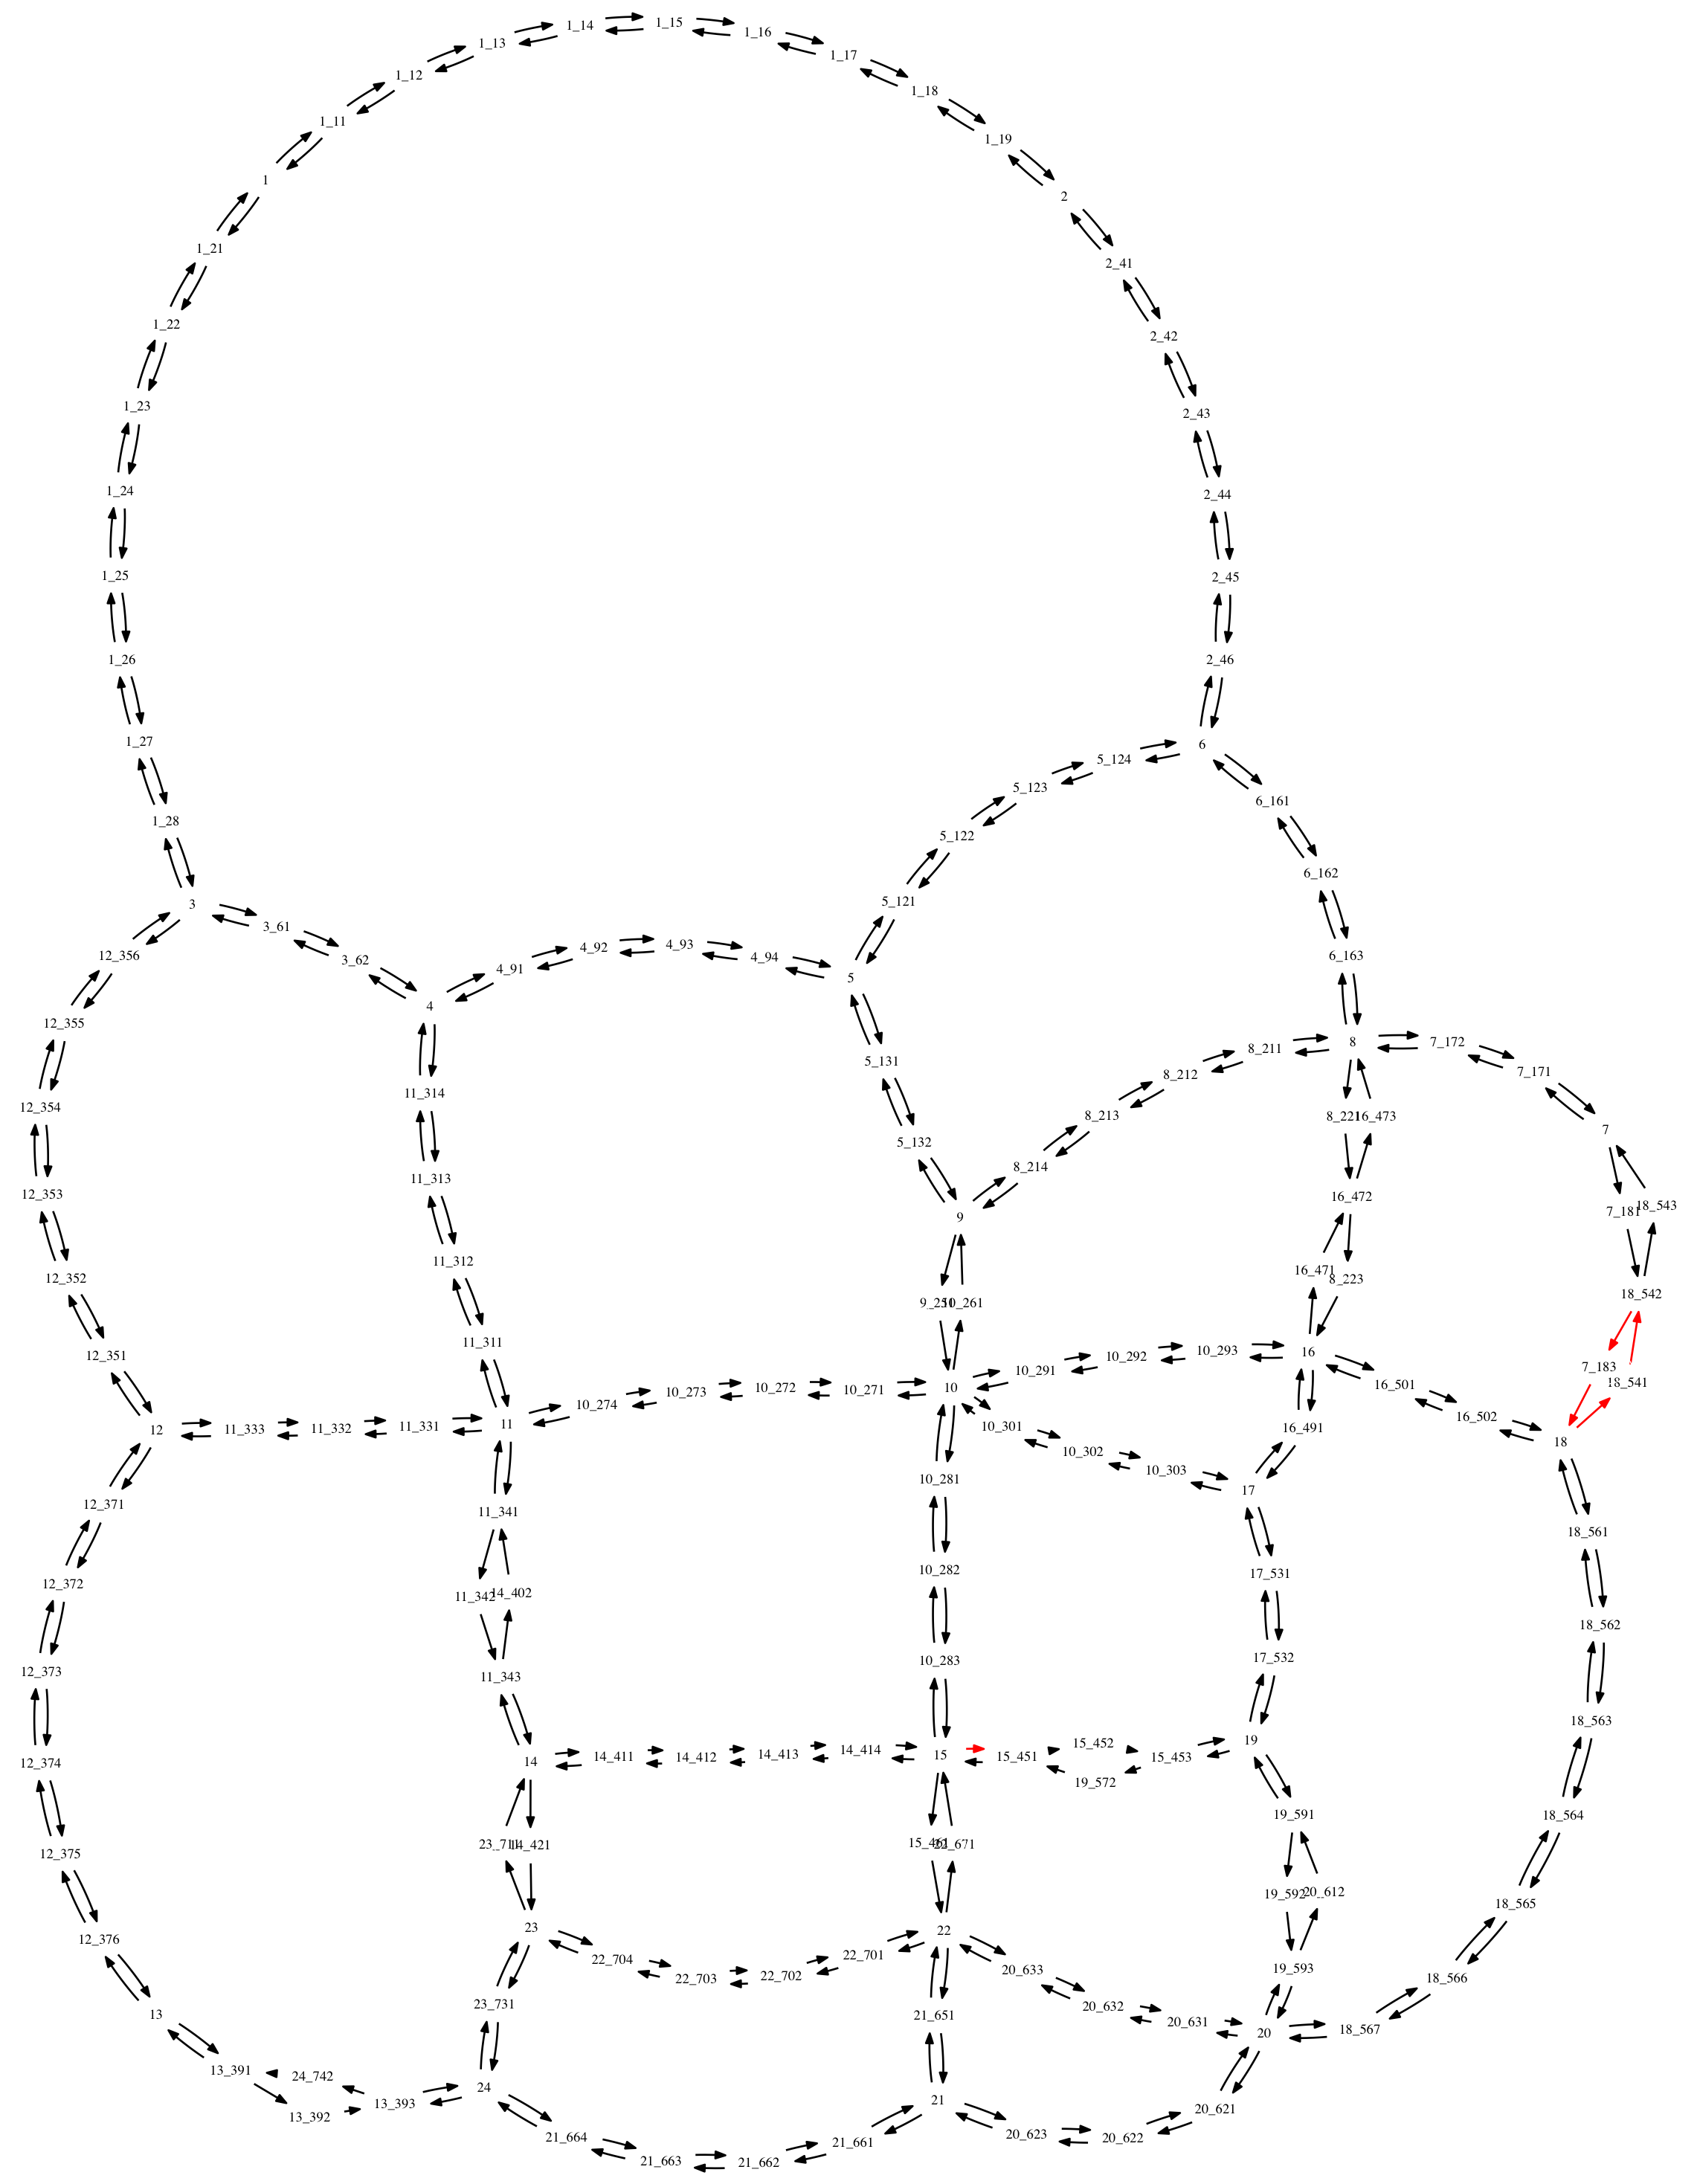
\includegraphics[totalheight=0.550\textheight, angle=90]{img/sioux-out/10/network2}};
	
	\draw[red,ultra thick] (7.7,9.5) rectangle (9.5,0 |- image.north);
%	\draw[red,ultra thick] (4.35,5.15) rectangle (6.75,8.0);
	\draw[red,ultra thick] (10.7,5.7) rectangle (11.5,6.7);
%	\draw[red,ultra thick] (5.3,0) rectangle (9.6,1.6);
\end{tikzpicture}
\caption{Sieć miasta Sioux Falls, rozwiązanie nr 10}
\label{fig:sioux10}
\end{figure}

\begin{figure}[htbp]
\centering
\begin{tikzpicture}
    \node[anchor=south west] (image) at (0,0)
    {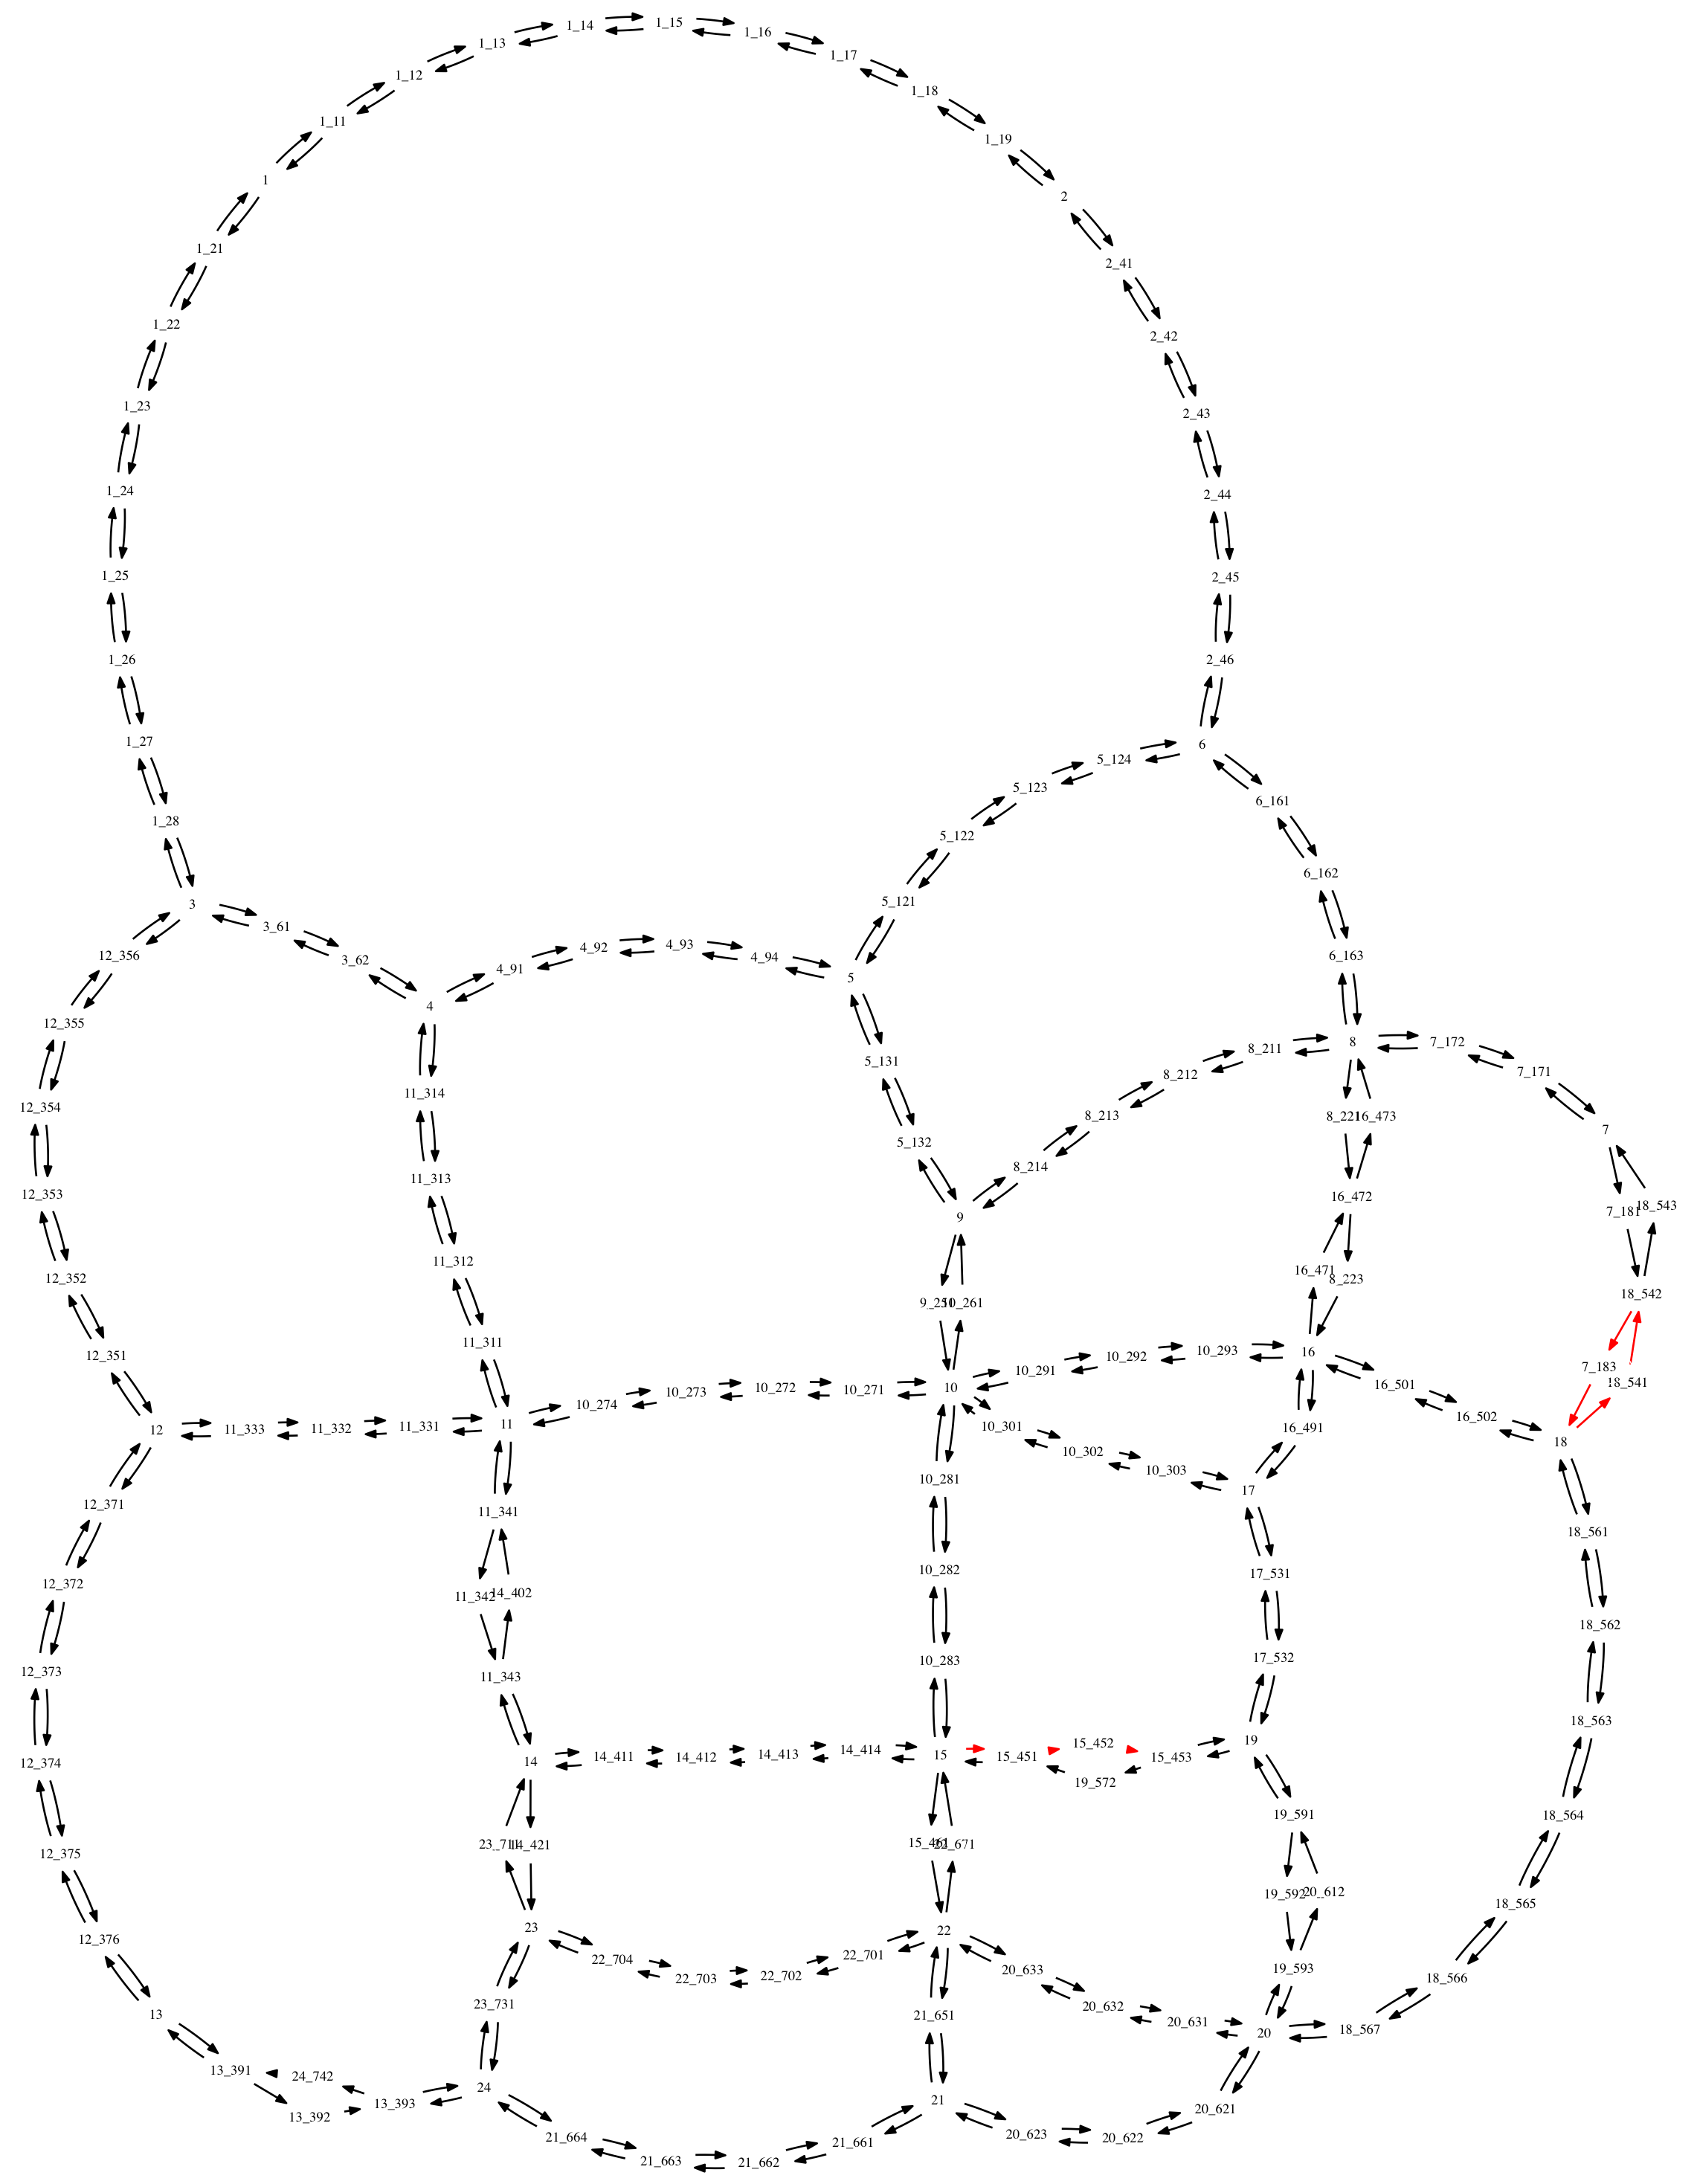
\includegraphics[totalheight=0.550\textheight, angle=90]{img/sioux-out/11/network2}};
	
	\draw[red,ultra thick] (7.7,9.5) rectangle (9.5,0 |- image.north);
%	\draw[red,ultra thick] (4.35,5.15) rectangle (6.75,8.0);
	\draw[red,ultra thick] (10.5,5.5) rectangle (11.8,7.7);
%	\draw[red,ultra thick] (5.3,0) rectangle (9.6,1.6);
\end{tikzpicture}
\caption{Sieć miasta Sioux Falls, rozwiązanie nr 11}
\label{fig:sioux11}
\end{figure}

\begin{figure}[htbp]
\centering
\begin{tikzpicture}
    \node[anchor=south west] (image) at (0,0)
    {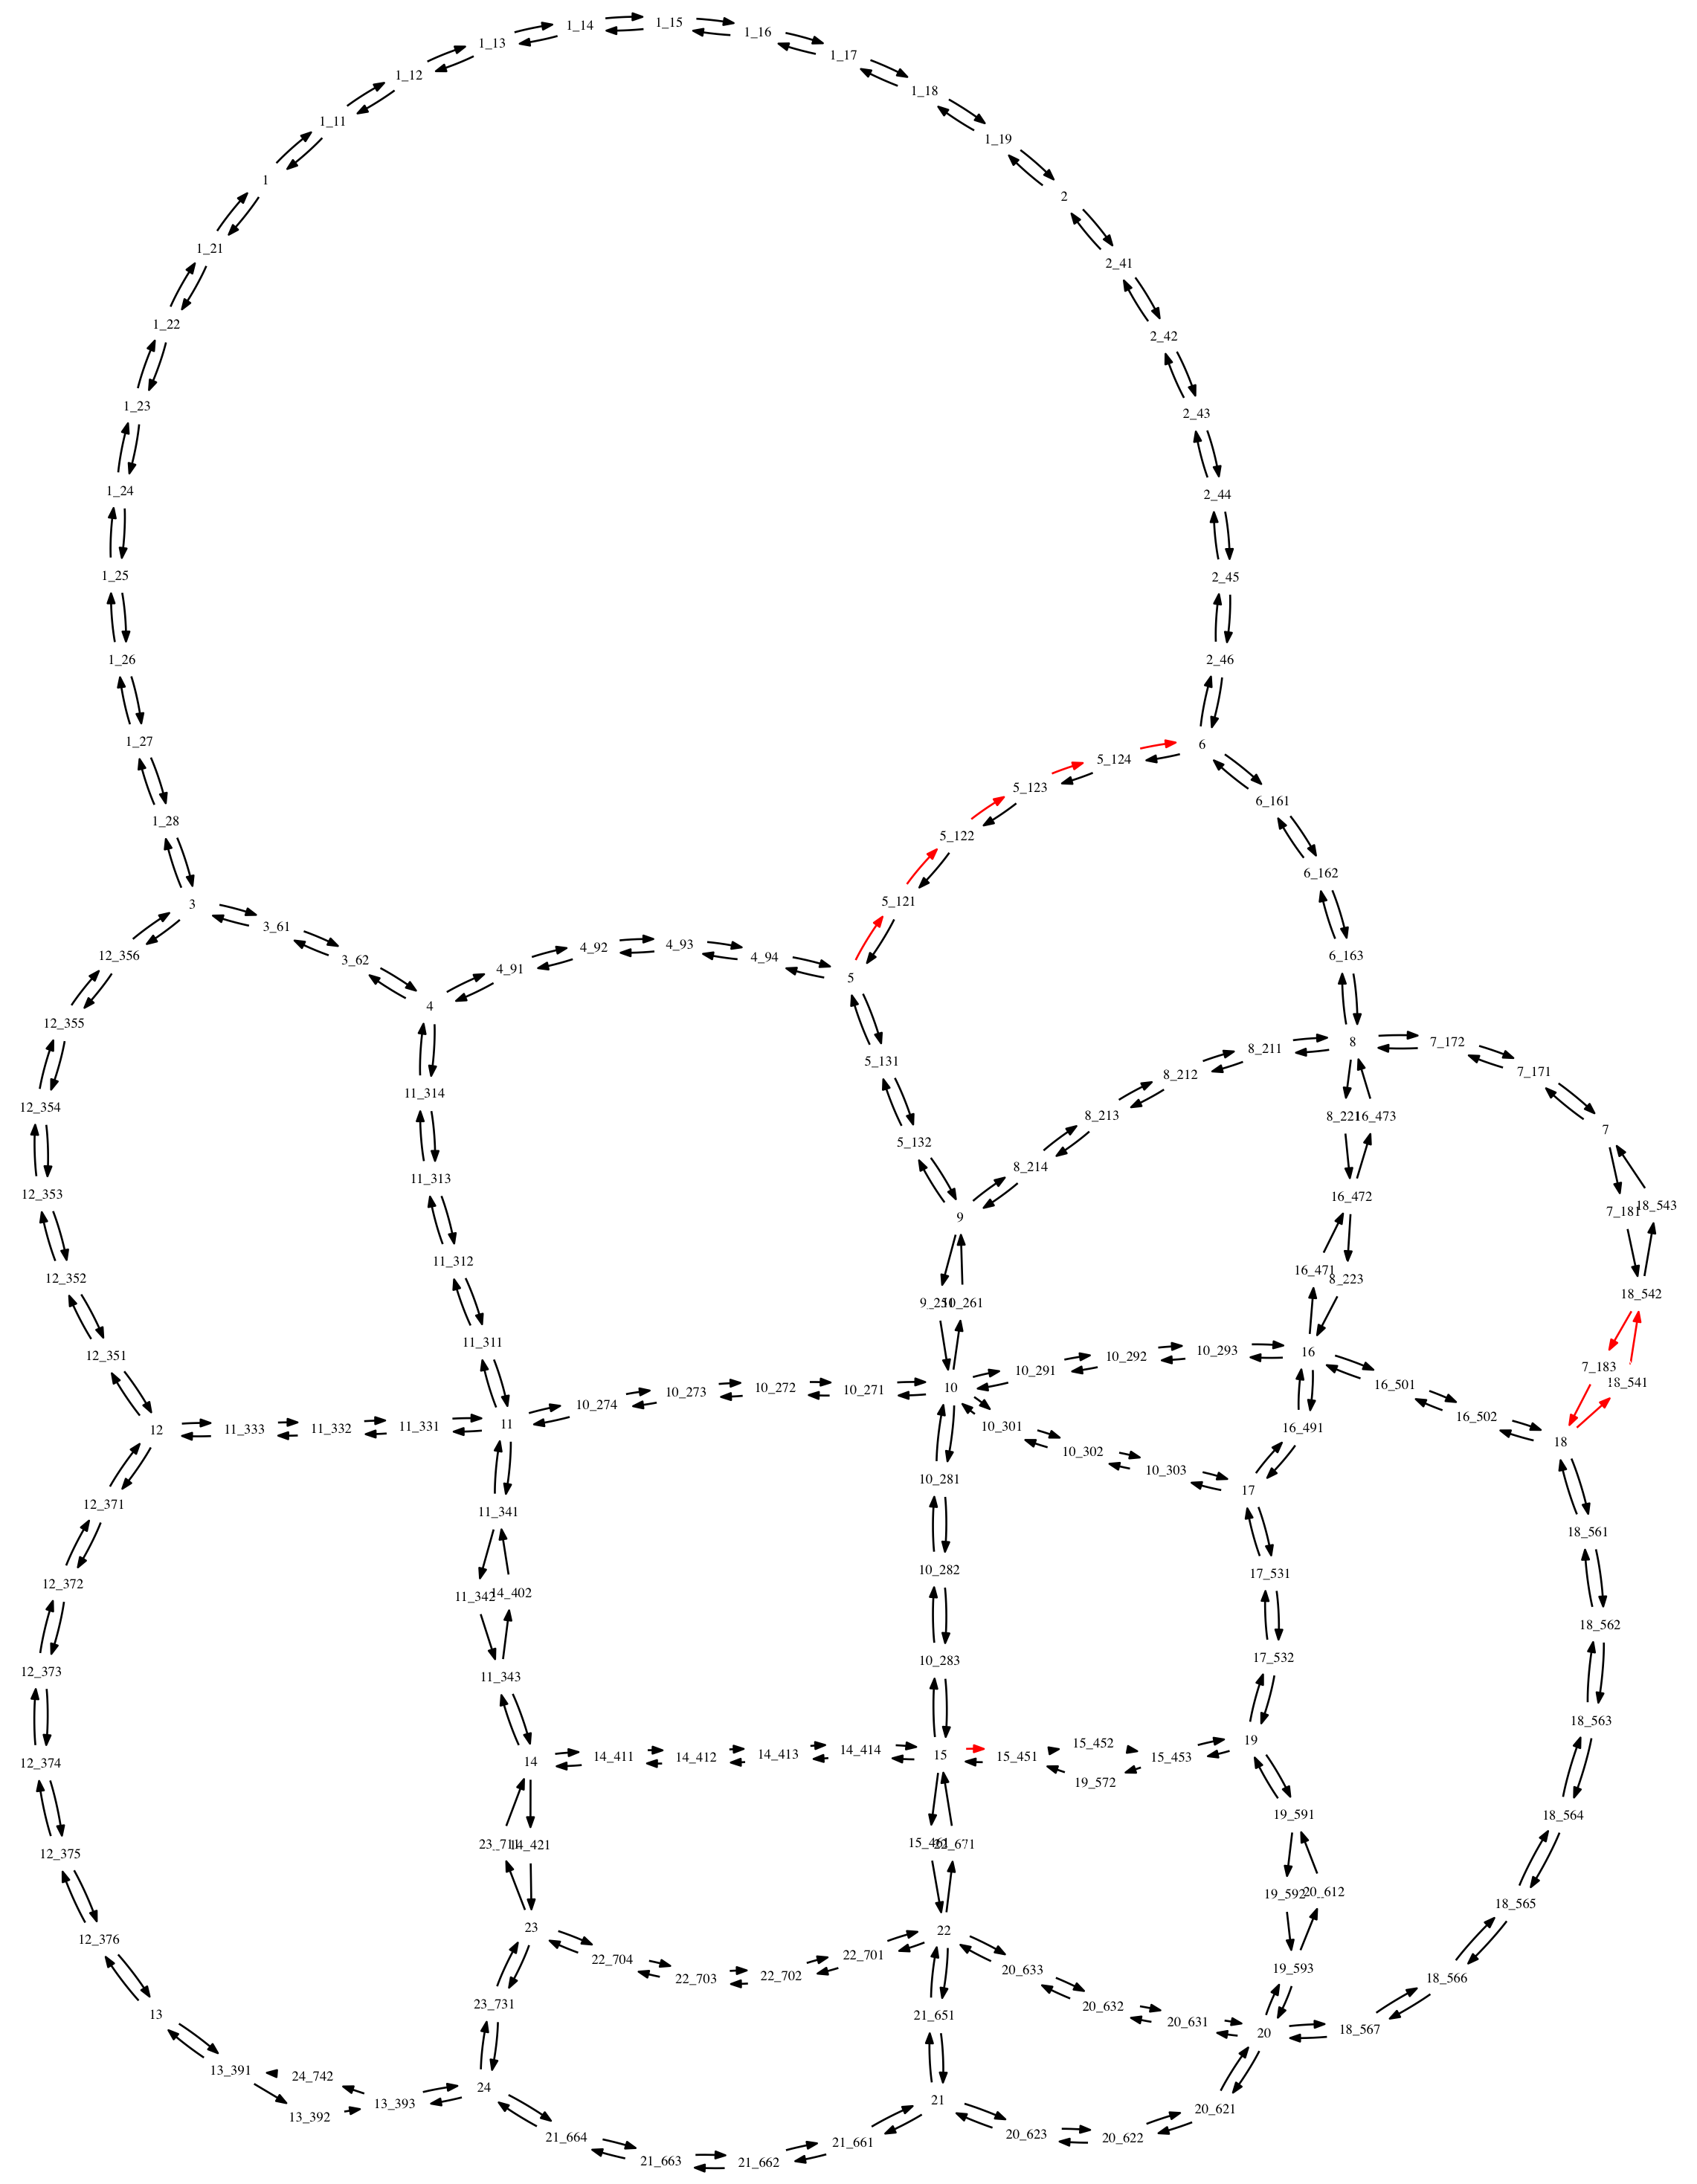
\includegraphics[totalheight=0.550\textheight, angle=90]{img/sioux-out/12/network2}};
	
	\draw[red,ultra thick] (7.7,9.5) rectangle (9.5,0 |- image.north);
	\draw[red,ultra thick] (4.35,5.15) rectangle (6.75,8.0);
	\draw[red,ultra thick] (10.7,5.7) rectangle (11.5,6.7);
%	\draw[red,ultra thick] (5.3,0) rectangle (9.6,1.6);
\end{tikzpicture}
\caption{Sieć miasta Sioux Falls, rozwiązanie nr 12}
\label{fig:sioux12}
\end{figure}

\begin{figure}[htbp]
\centering
\begin{tikzpicture}
    \node[anchor=south west] (image) at (0,0)
    {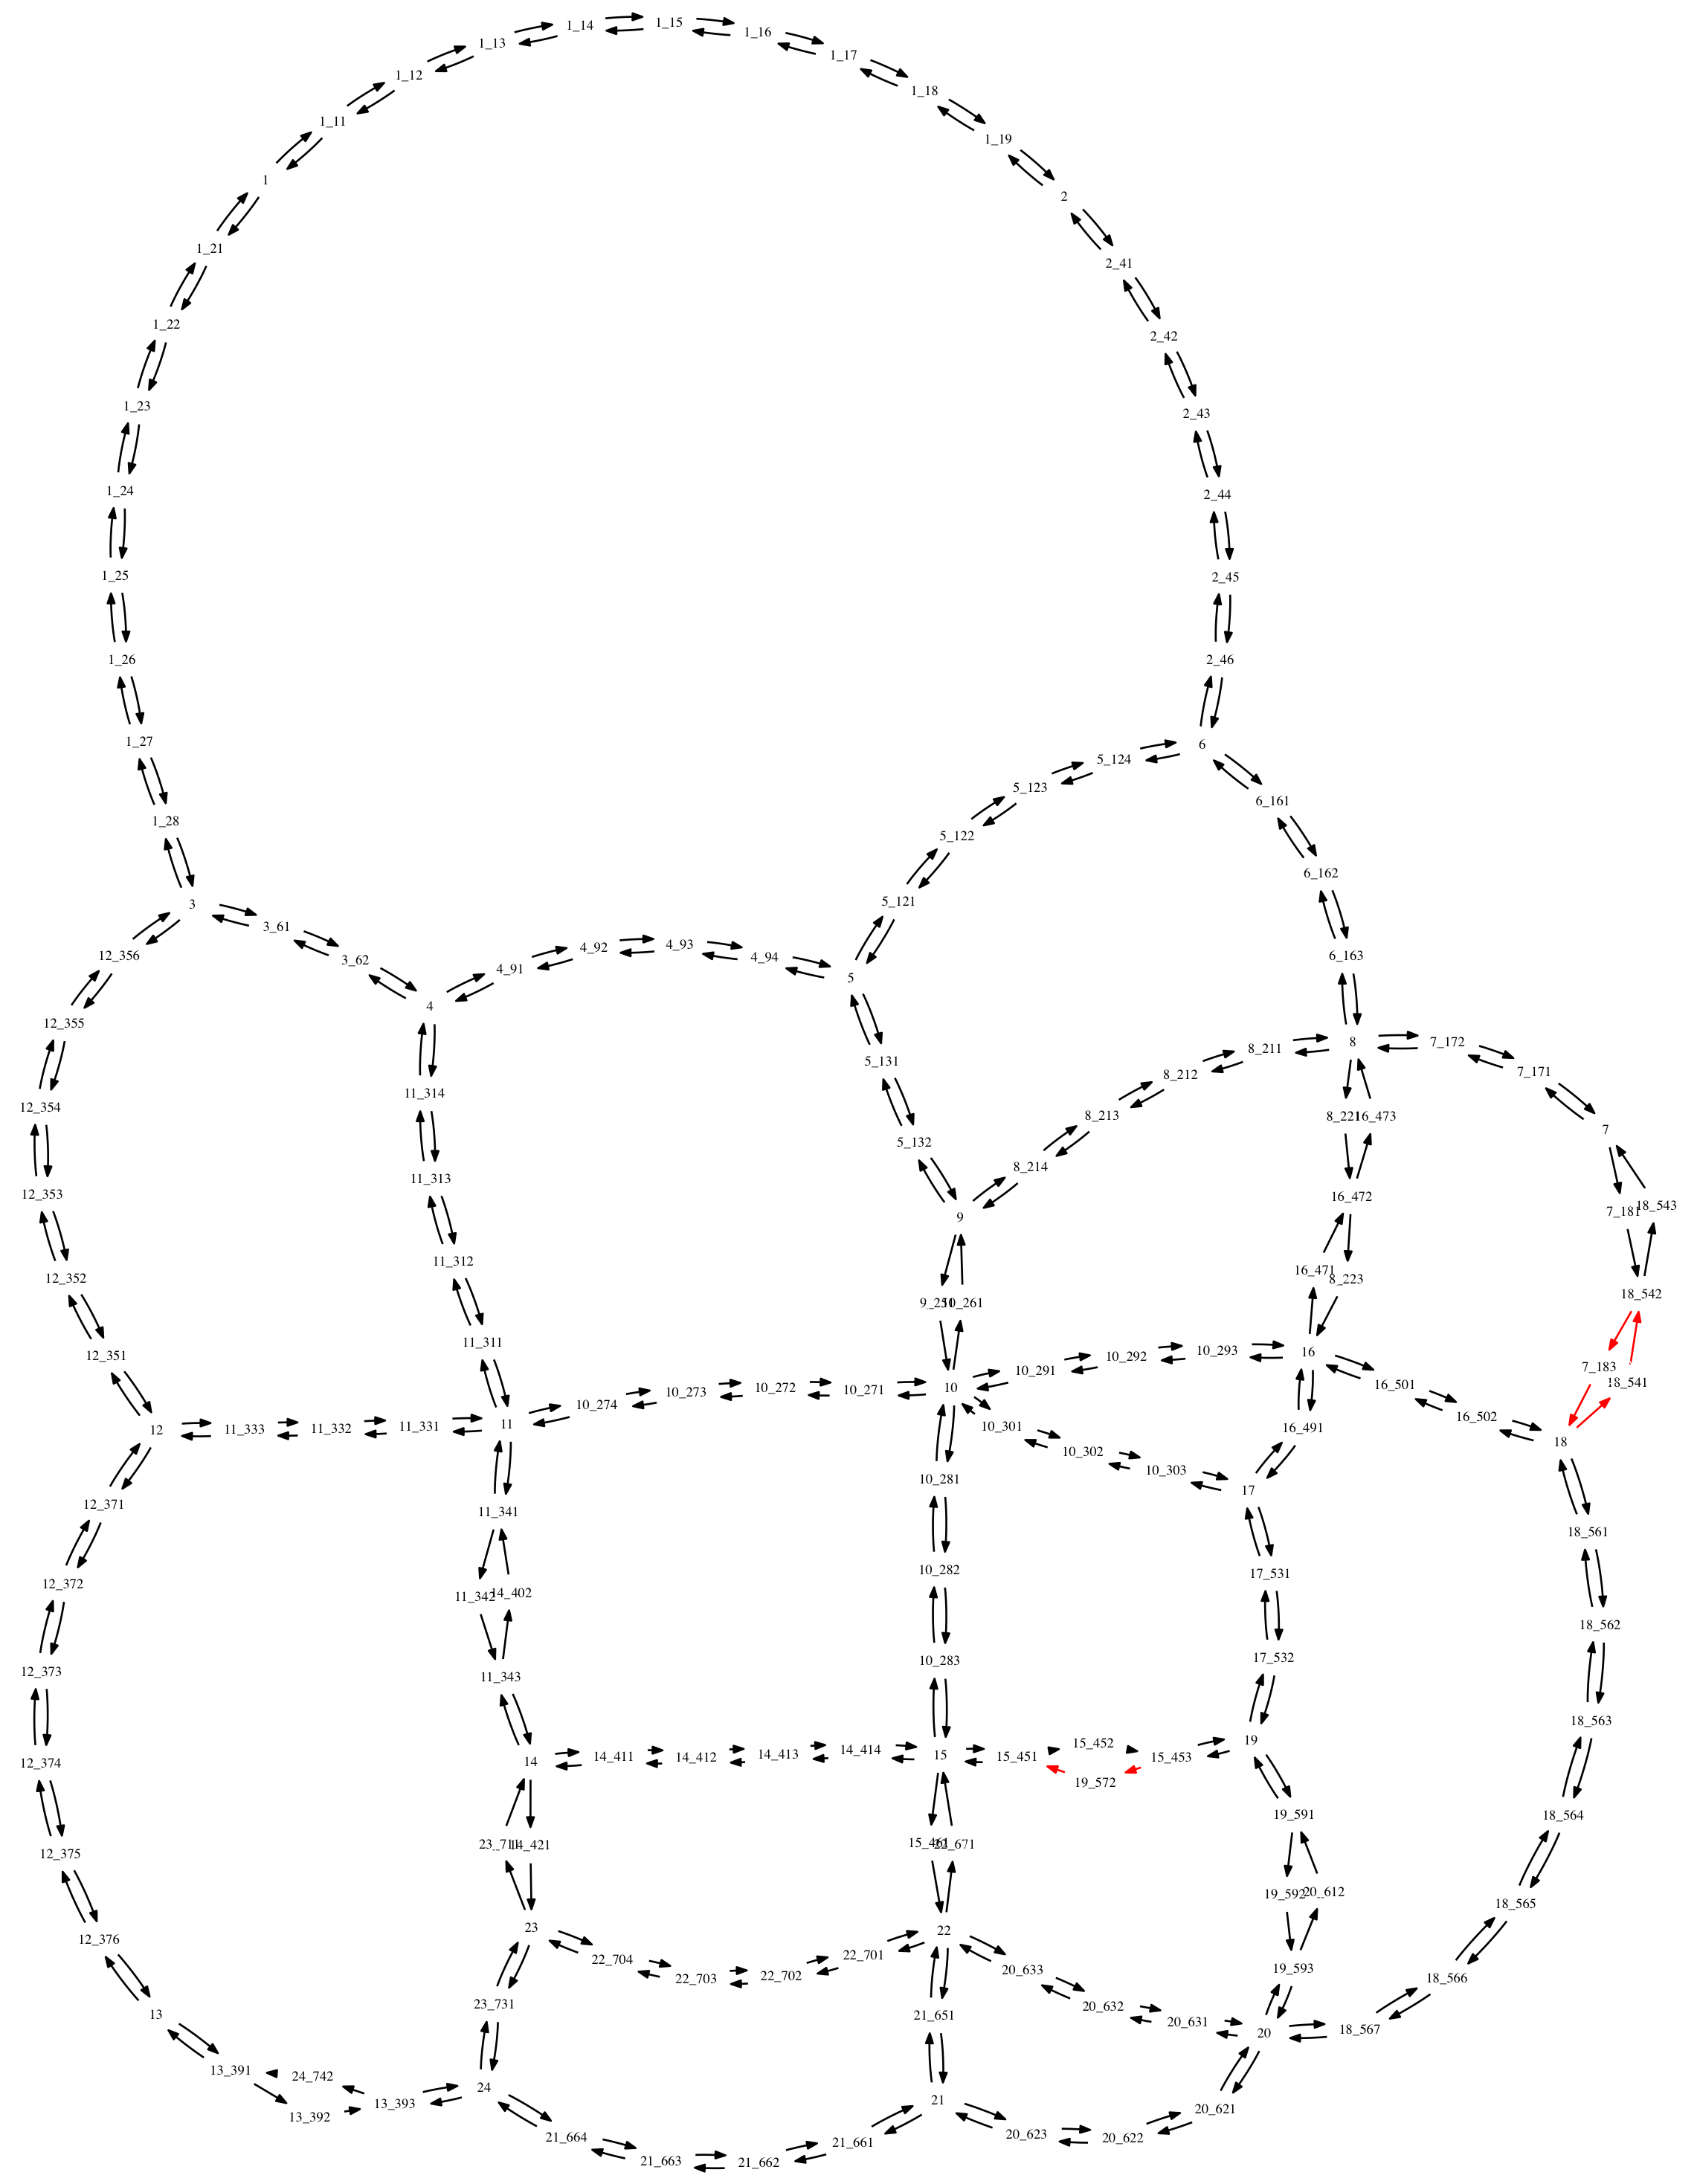
\includegraphics[totalheight=0.550\textheight, angle=90]{img/sioux-out/13/network2}};
	
	\draw[red,ultra thick] (7.7,9.5) rectangle (9.5,0 |- image.north);
%	\draw[red,ultra thick] (4.35,5.15) rectangle (6.75,8.0);
	\draw[red,ultra thick] (10.4,6.2) rectangle (11.8,7.8);
%	\draw[red,ultra thick] (5.3,0) rectangle (9.6,1.6);
\end{tikzpicture}
\caption{Sieć miasta Sioux Falls, rozwiązanie nr 13}
\label{fig:sioux13}
\end{figure}

\begin{figure}[htbp]
\centering
\begin{tikzpicture}
    \node[anchor=south west] (image) at (0,0)
    {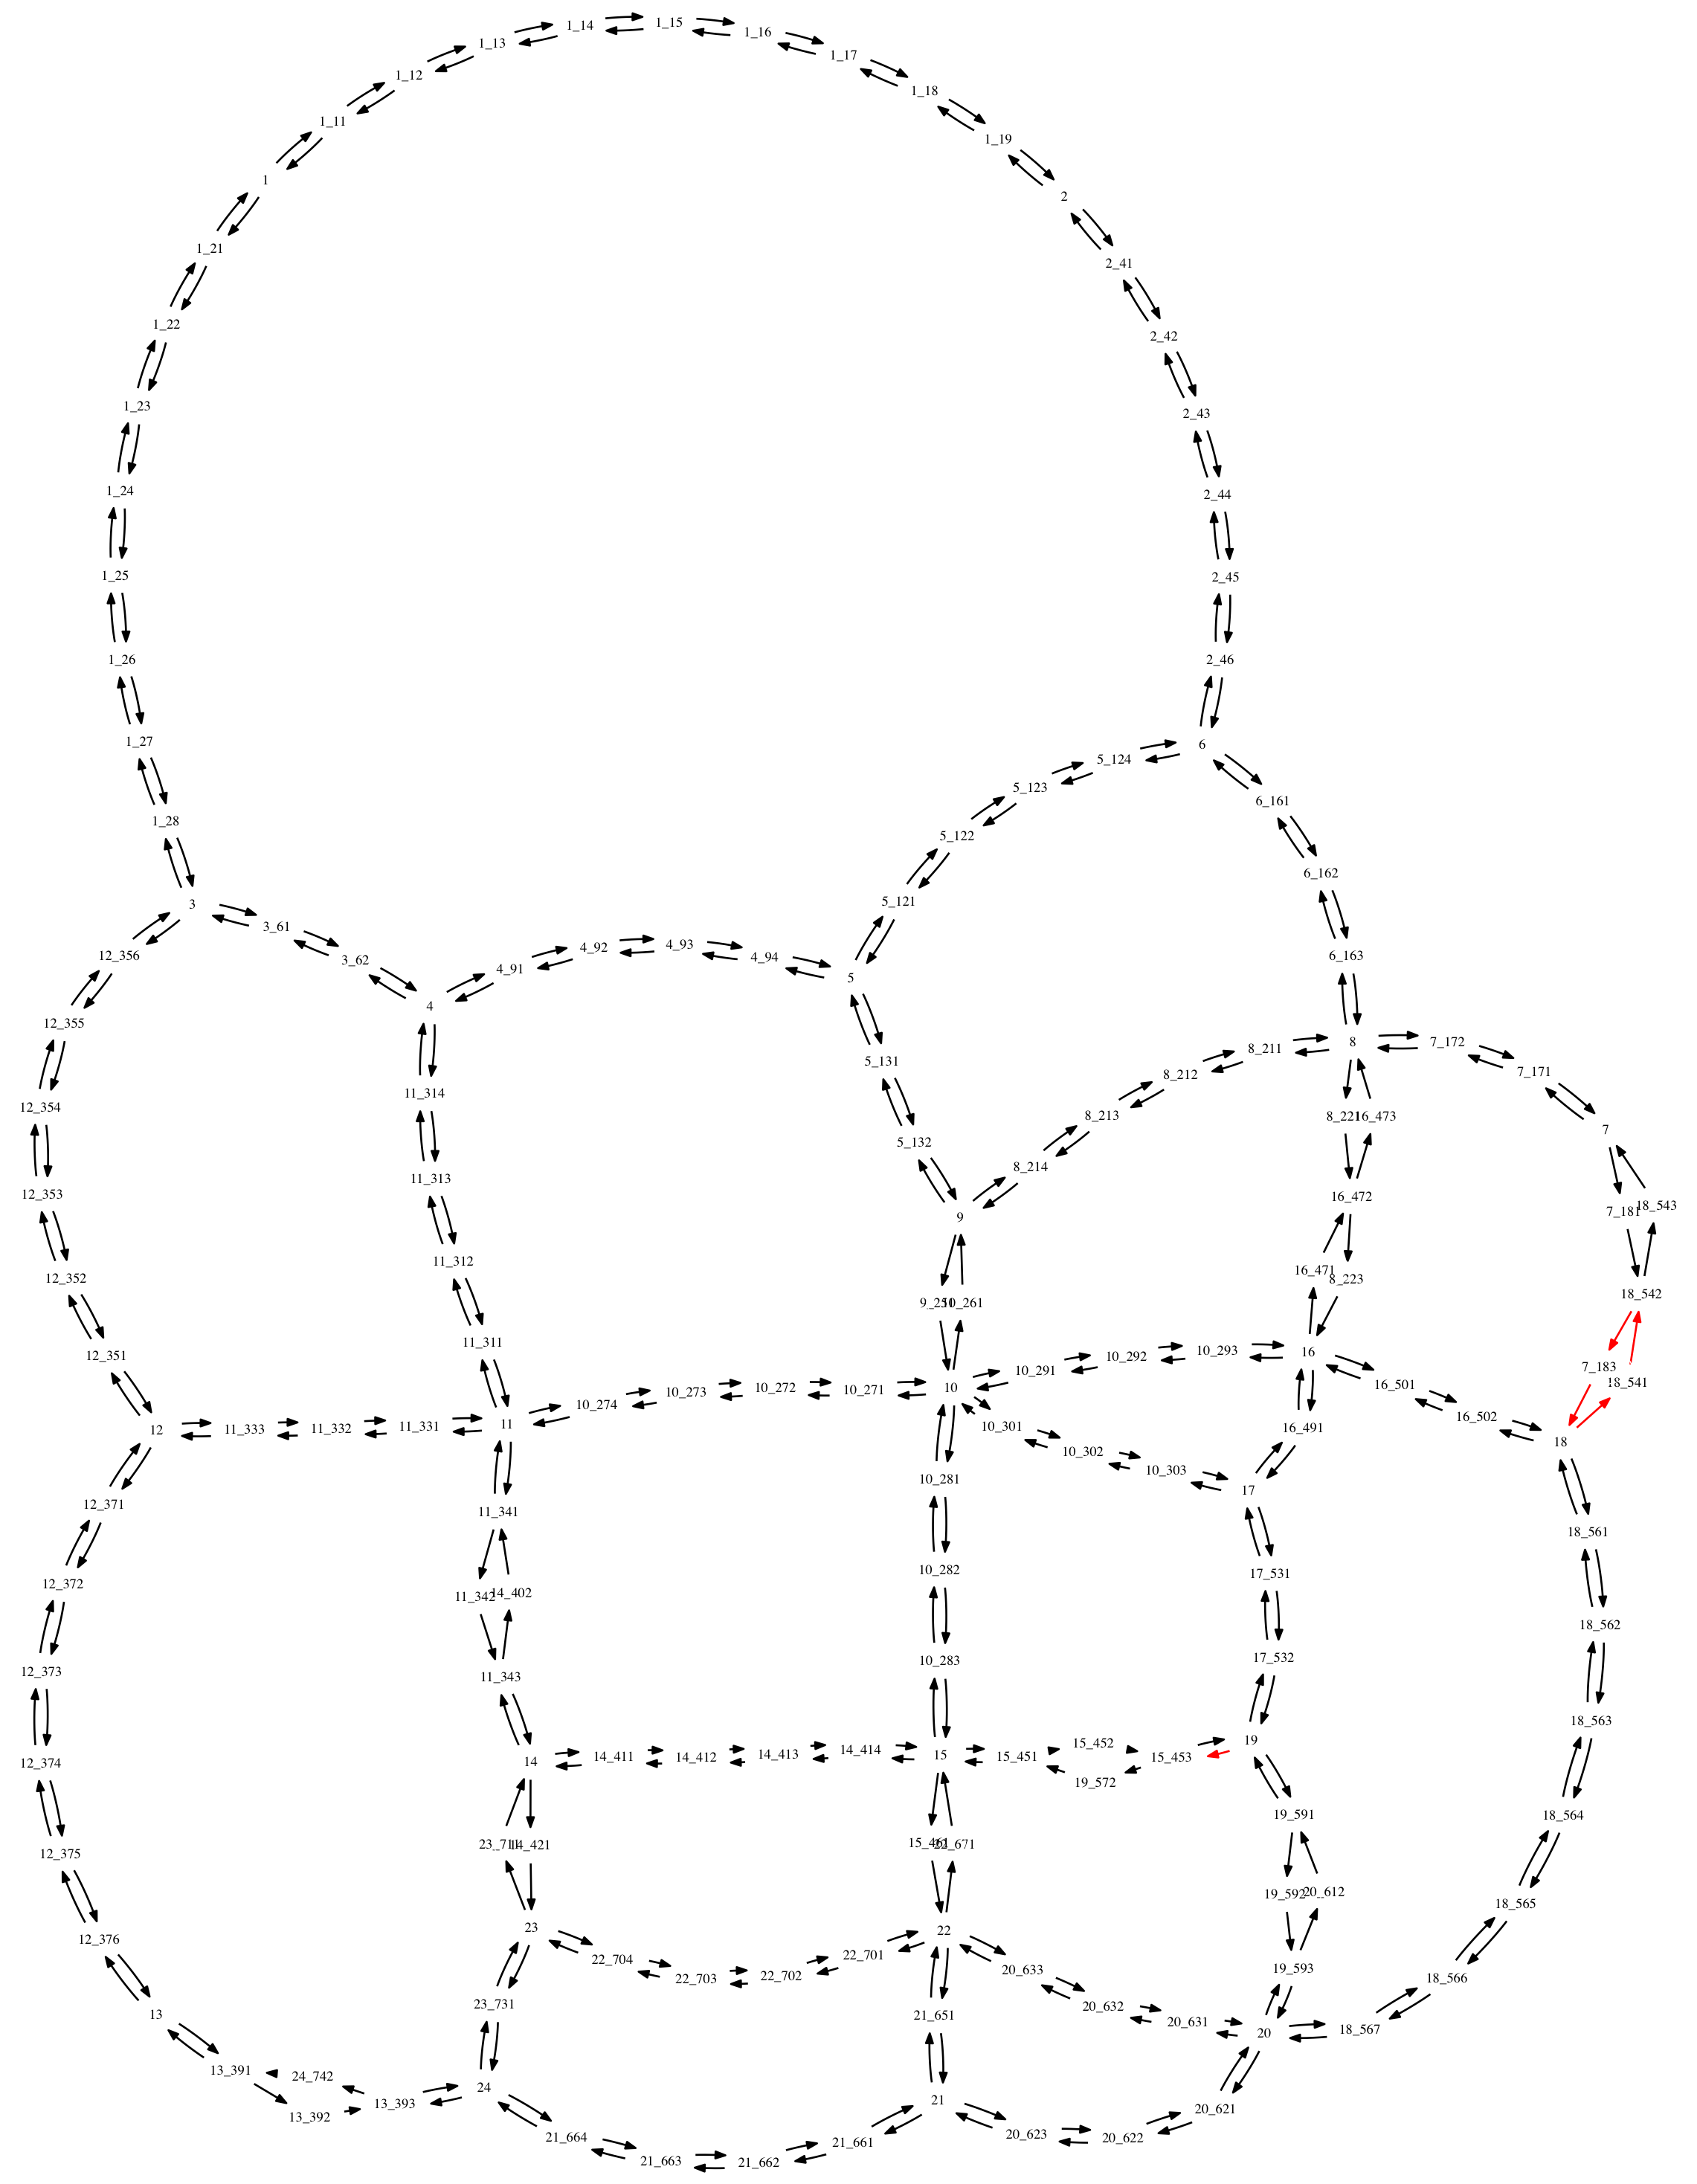
\includegraphics[totalheight=0.550\textheight, angle=90]{img/sioux-out/14/network2}};
	
	\draw[red,ultra thick] (7.7,9.5) rectangle (9.5,0 |- image.north);
%	\draw[red,ultra thick] (4.35,5.15) rectangle (6.75,8.0);
	\draw[red,ultra thick] (10.7,7.2) rectangle (11.4,8.3);
%	\draw[red,ultra thick] (5.3,0) rectangle (9.6,1.6);
\end{tikzpicture}
\caption{Sieć miasta Sioux Falls, rozwiązanie nr 14}
\label{fig:sioux14}
\end{figure}

\begin{figure}[htbp]
\centering
\begin{tikzpicture}
    \node[anchor=south west] (image) at (0,0)
    {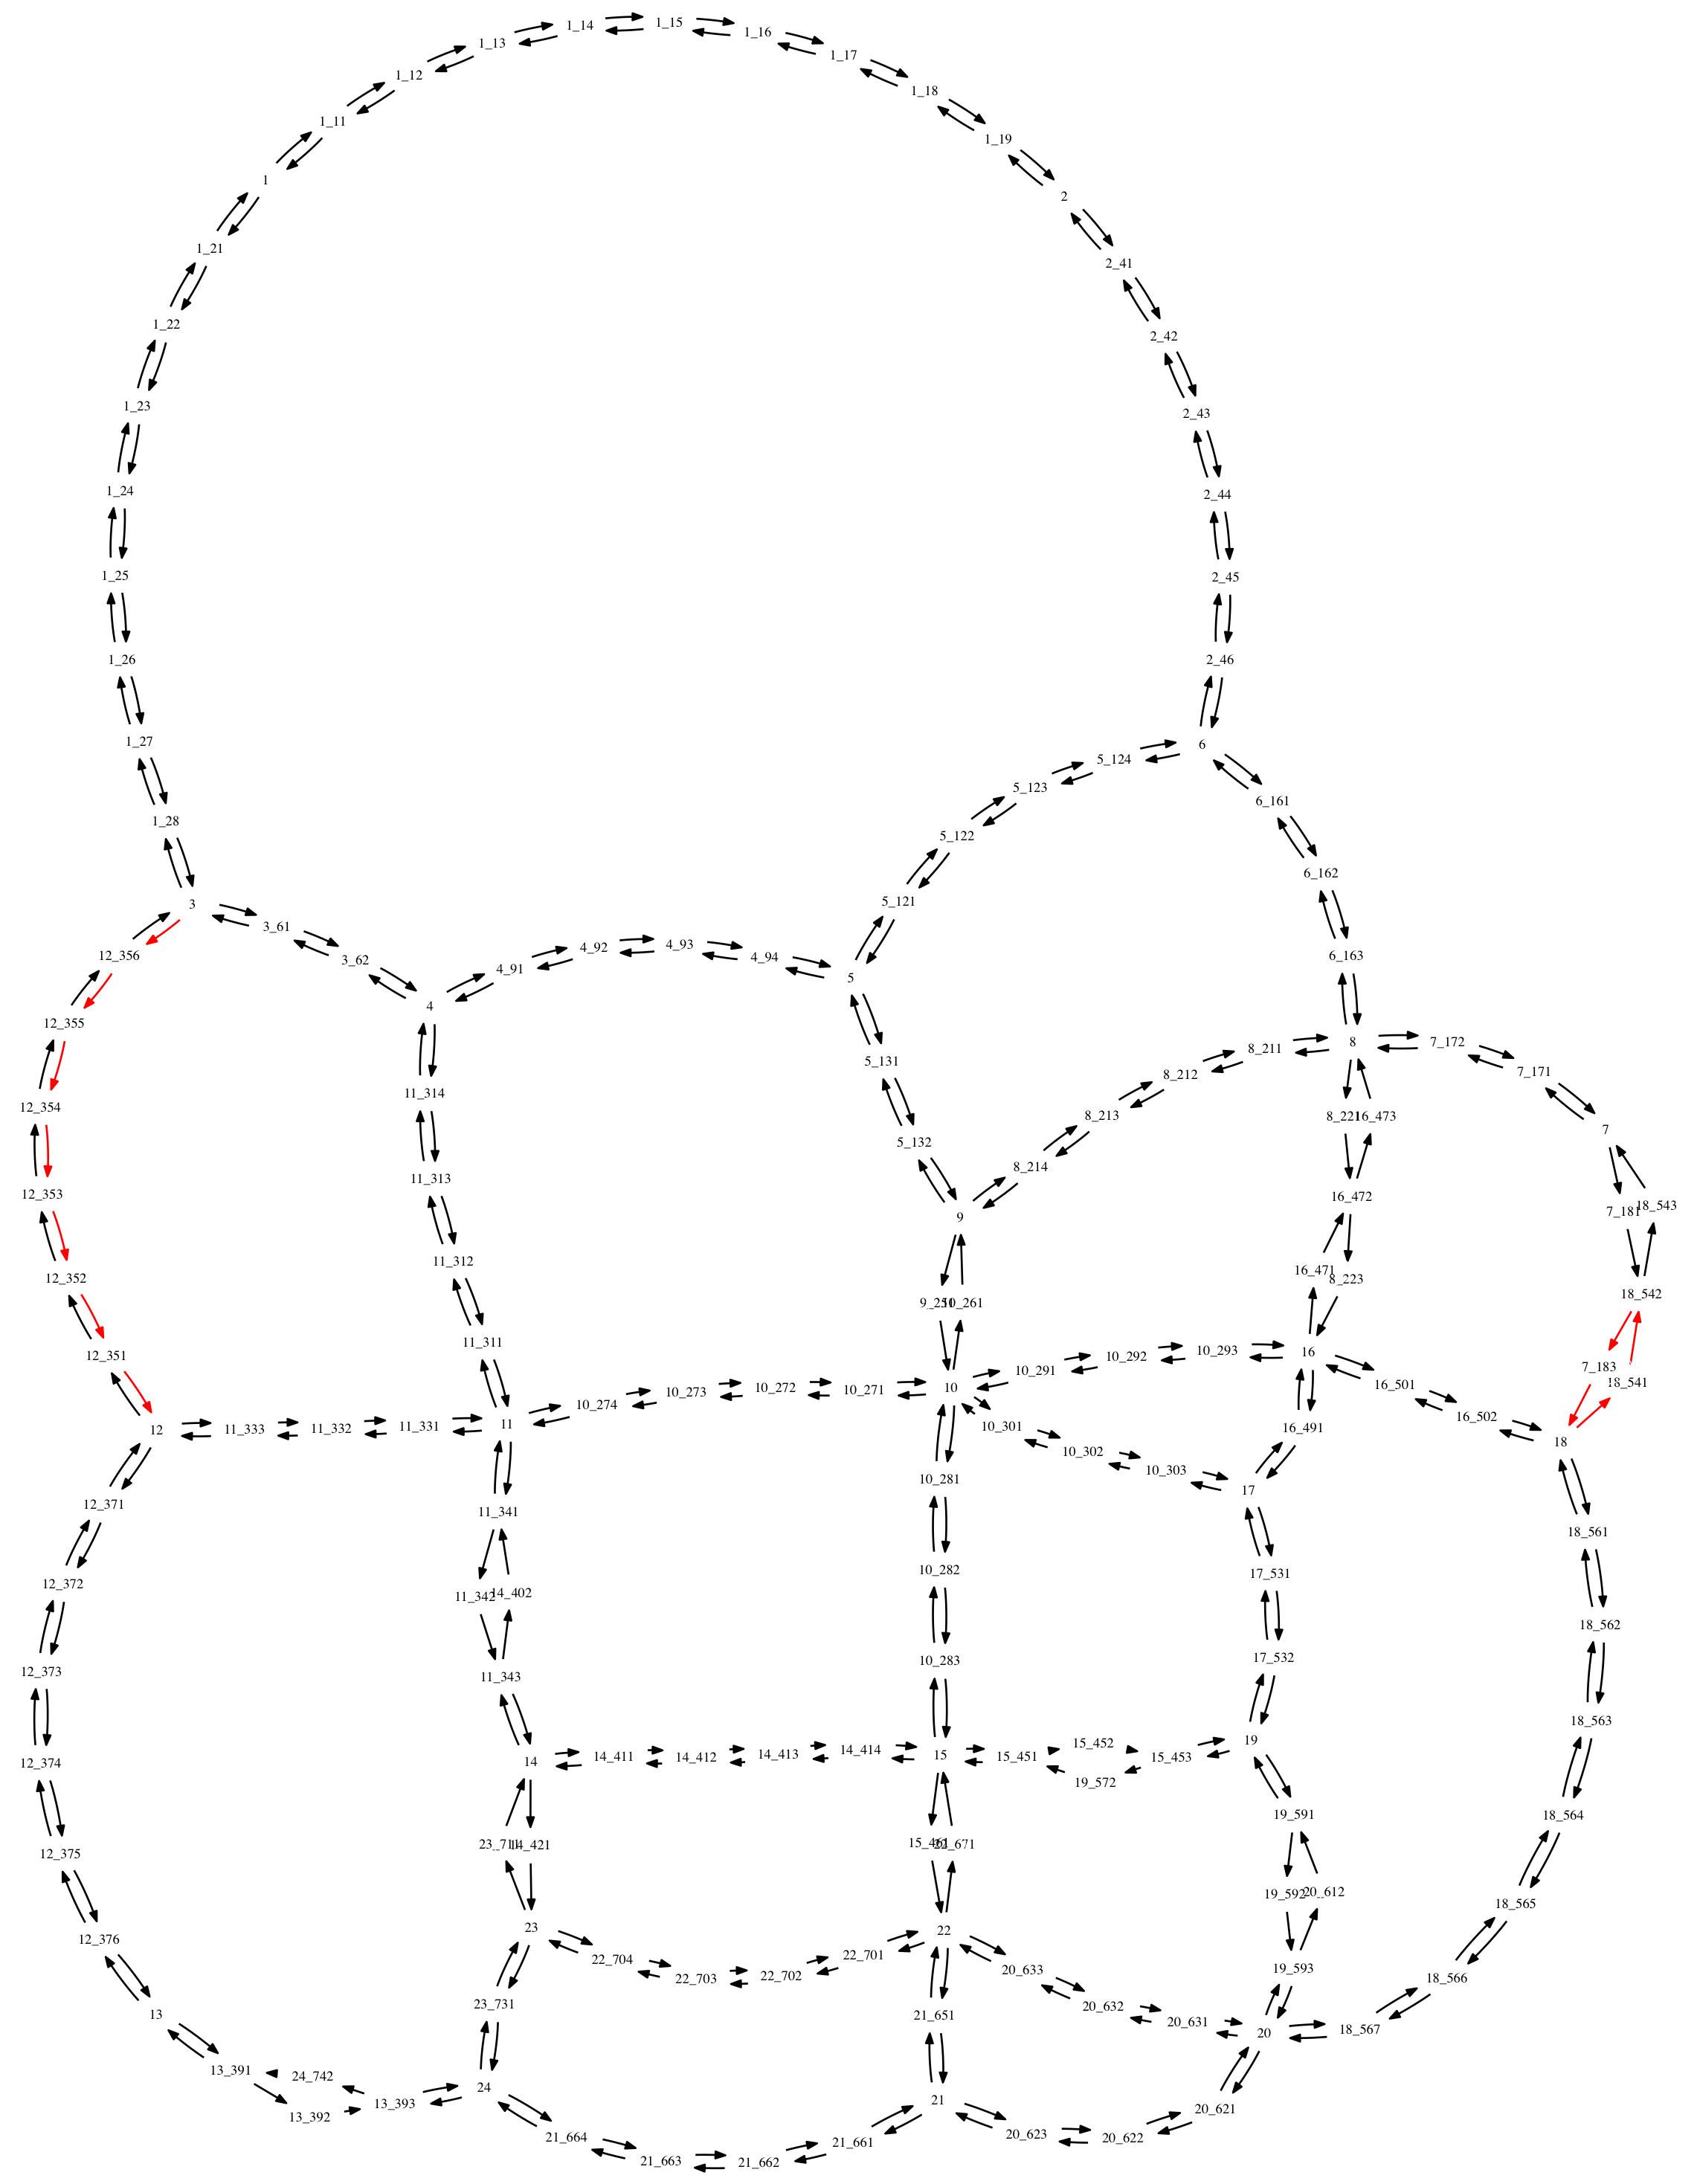
\includegraphics[totalheight=0.550\textheight, angle=90]{img/sioux-out/15/network2}};
	
	\draw[red,ultra thick] (7.7,9.5) rectangle (9.5,0 |- image.north);
%	\draw[red,ultra thick] (4.35,5.15) rectangle (6.75,8.0);
%	\draw[red,ultra thick] (10.4,5.5) rectangle (11.8,8.3);
	\draw[red,ultra thick] (5.3,0) rectangle (9.6,1.6);
\end{tikzpicture}
\caption{Sieć miasta Sioux Falls, rozwiązanie nr 15}
\label{fig:sioux15}
\end{figure}

\begin{figure}[htbp]
\centering
\begin{tikzpicture}
    \node[anchor=south west] (image) at (0,0)
    {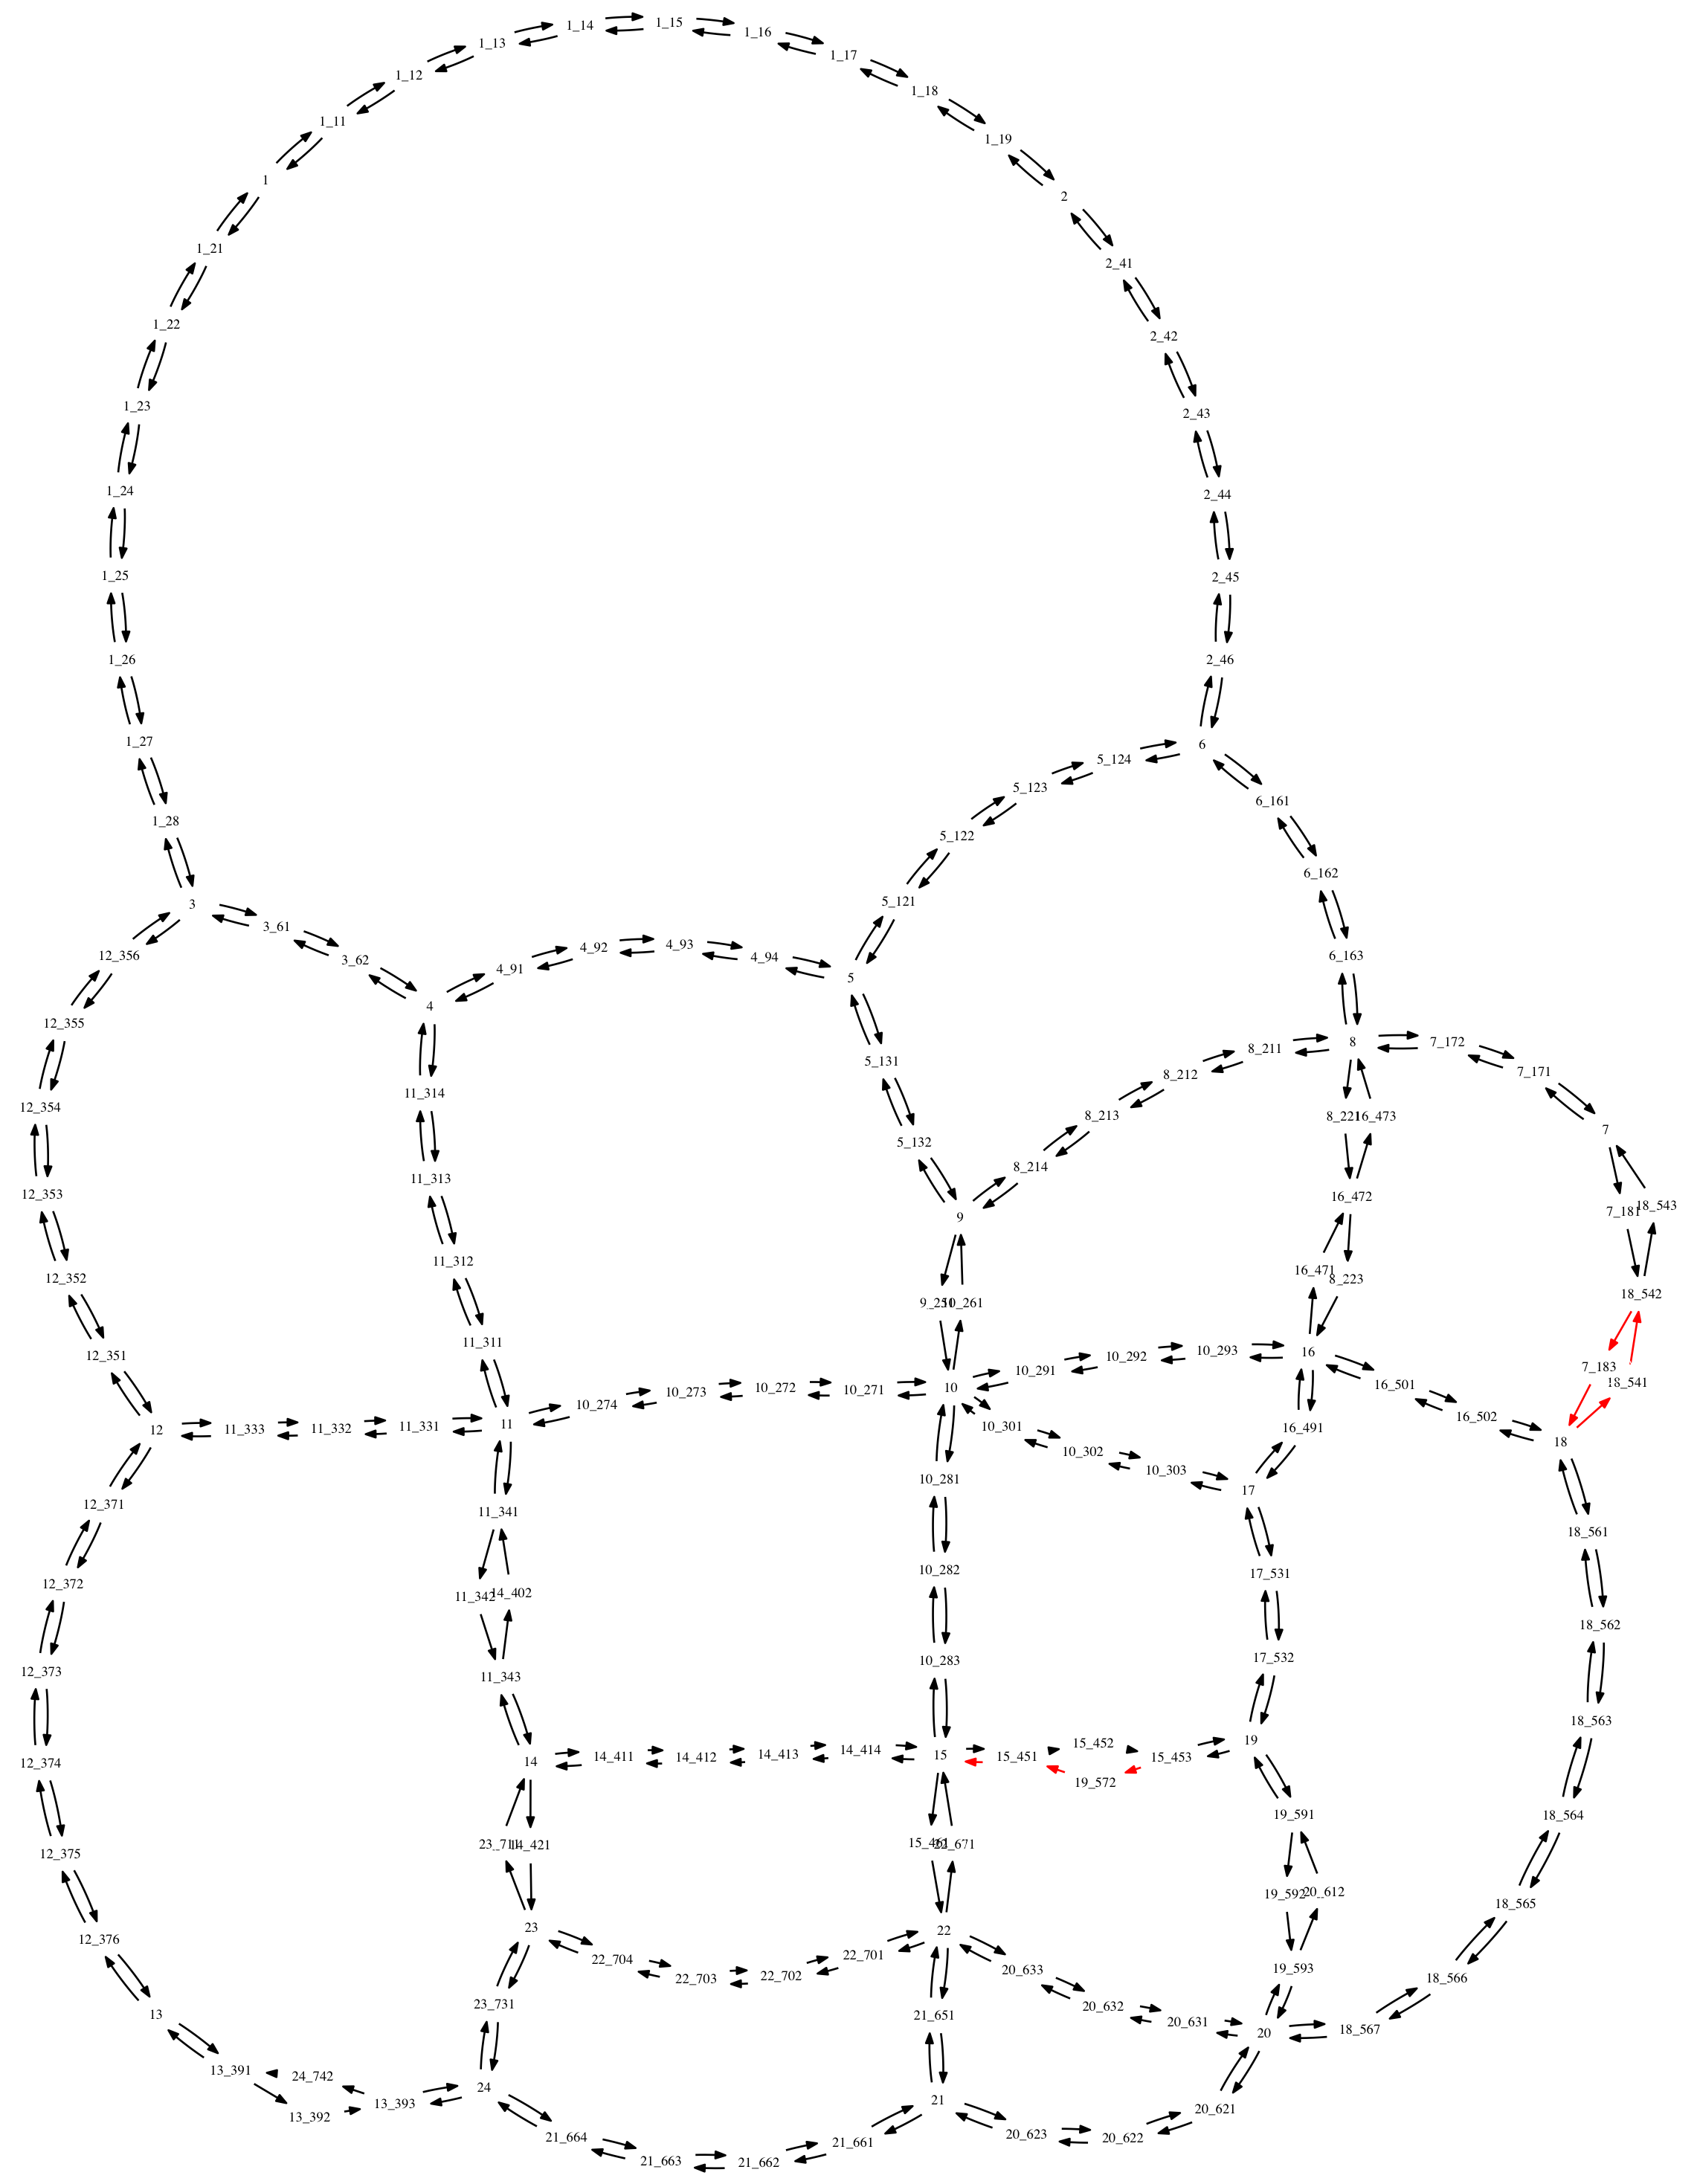
\includegraphics[totalheight=0.550\textheight, angle=90]{img/sioux-out/16/network2}};
	
	\draw[red,ultra thick] (7.7,9.5) rectangle (9.5,0 |- image.north);
%	\draw[red,ultra thick] (4.35,5.15) rectangle (6.75,8.0);
	\draw[red,ultra thick] (10.5,5.8) rectangle (11.7,7.5);
%	\draw[red,ultra thick] (5.3,0) rectangle (9.6,1.6);
\end{tikzpicture}
\caption{Sieć miasta Sioux Falls, rozwiązanie nr 16}
\label{fig:sioux16}
\end{figure}

\begin{figure}[htbp]
\centering
\begin{tikzpicture}
    \node[anchor=south west] (image) at (0,0)
    {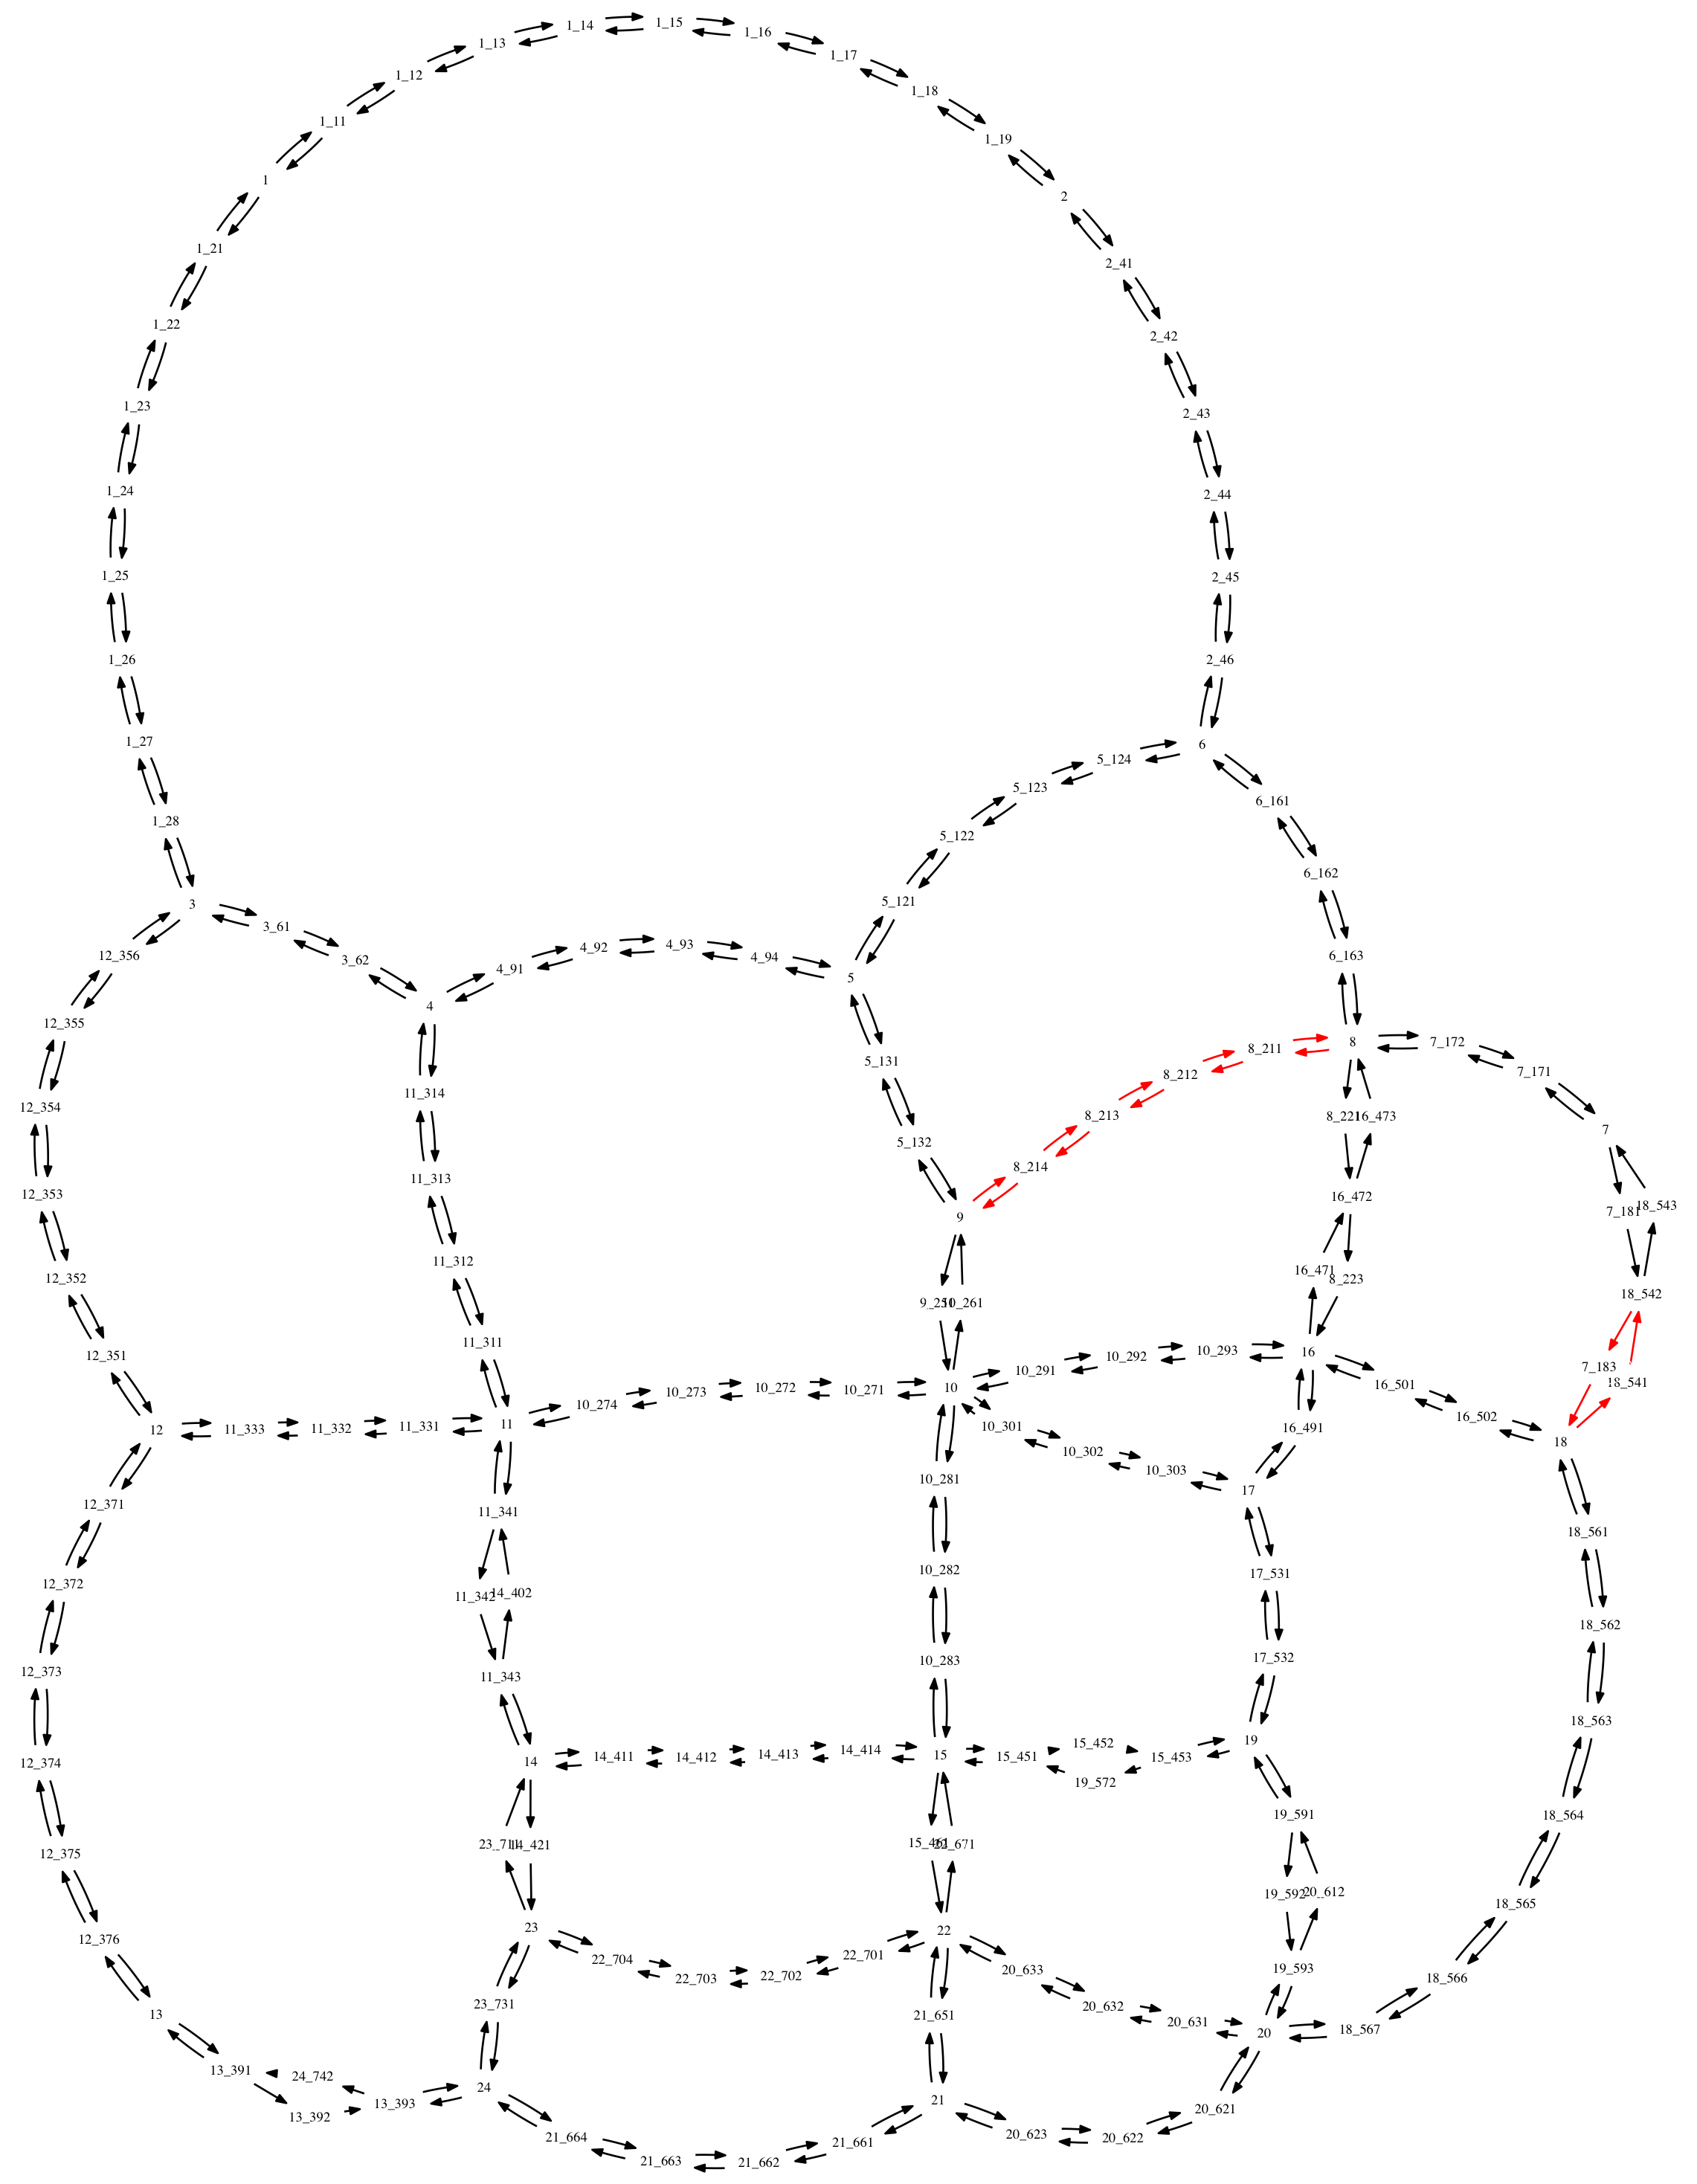
\includegraphics[totalheight=0.550\textheight, angle=90]{img/sioux-out/17/network2}};
	
	\draw[red,ultra thick] (7.7,9.5) rectangle (9.5,0 |- image.north);
	\draw[red,ultra thick] (6.3,5.8) rectangle (8,8.7);
%	\draw[red,ultra thick] (10.4,5.5) rectangle (11.8,8.3);
%	\draw[red,ultra thick] (5.3,0) rectangle (9.6,1.6);
\end{tikzpicture}
\caption{Sieć miasta Sioux Falls, rozwiązanie nr 17}
\label{fig:sioux17}
\end{figure}

\clearpage
\section{Analiza uzyskanych wyników}\label{rozdz.analiza_uzyskanych_wynikow}
Pierwszym krokiem, który pomaga w~analizie otrzymanych wyników jest ich zgrupowanie. Dość intuicyjnym jest grupowanie w~zbiory zamykające podobne obszary (węzły). Wyniki należy interpretować z~uwzględnieniem natężenia ruchu panującego w~mieście oraz rozkładu budynków. Informacje te zostały przybliżone w~podrozdziale~\ref{rozdz.opis_siouxfalls} Natężenie ruchu prezentowane jest na rysunkach \ref{fig:siouxfalls_natezenie_1} i~\ref{fig:siouxfalls_natezenie_2}, natomiast rozkład budynków znajduje się na rysunku \ref{fig:siouxfalls_budynki}

,,Na pierwszy rzut oka'' widać wyraźną zbieżność w~jednym rejonie. Niestety, choć zdecydowanie musi mieć on wpływ na poprawę czasu symulacji, nie wydaje się on punktem ,,strategicznym'' komunikacji w~mieście. Mowa oczywiście o~zamknięciu węzłów między $18$ i~$18\_542$ (zaznaczony fragment na rysunku~\ref{fig:frag_1}, obrócony o~$90^{\circ}$ w~lewo). Analizując ten fragment pod kątem rozkładu budynków w~mieście, można zauważyć duże skupienie w~pobliżu tego węzła. Bardzo prawdopodobnym jest tutaj wpływ zamknięcia tych ulic na odległość domostw od najbliższego, możliwego punktu zostawienia samochodu. Podczas zamknięcia tego fragmentu, nastąpiło wydłużenie odcinka pokonywanego bez samochodu dla wielu mieszkańców. Mogło to zmusić ich do wcześniejszego wychodzenia z~domu, oraz wcześniejszego rozpoczęcia podróży. To z~kolei wpłynęło na bardziej równomierne rozłożenie ruchu w~godzinach szczytu.

\begin{figure}[htbp]
\centering
\begin{tikzpicture}
    \node[anchor=south west] (image) at (0,0)
    {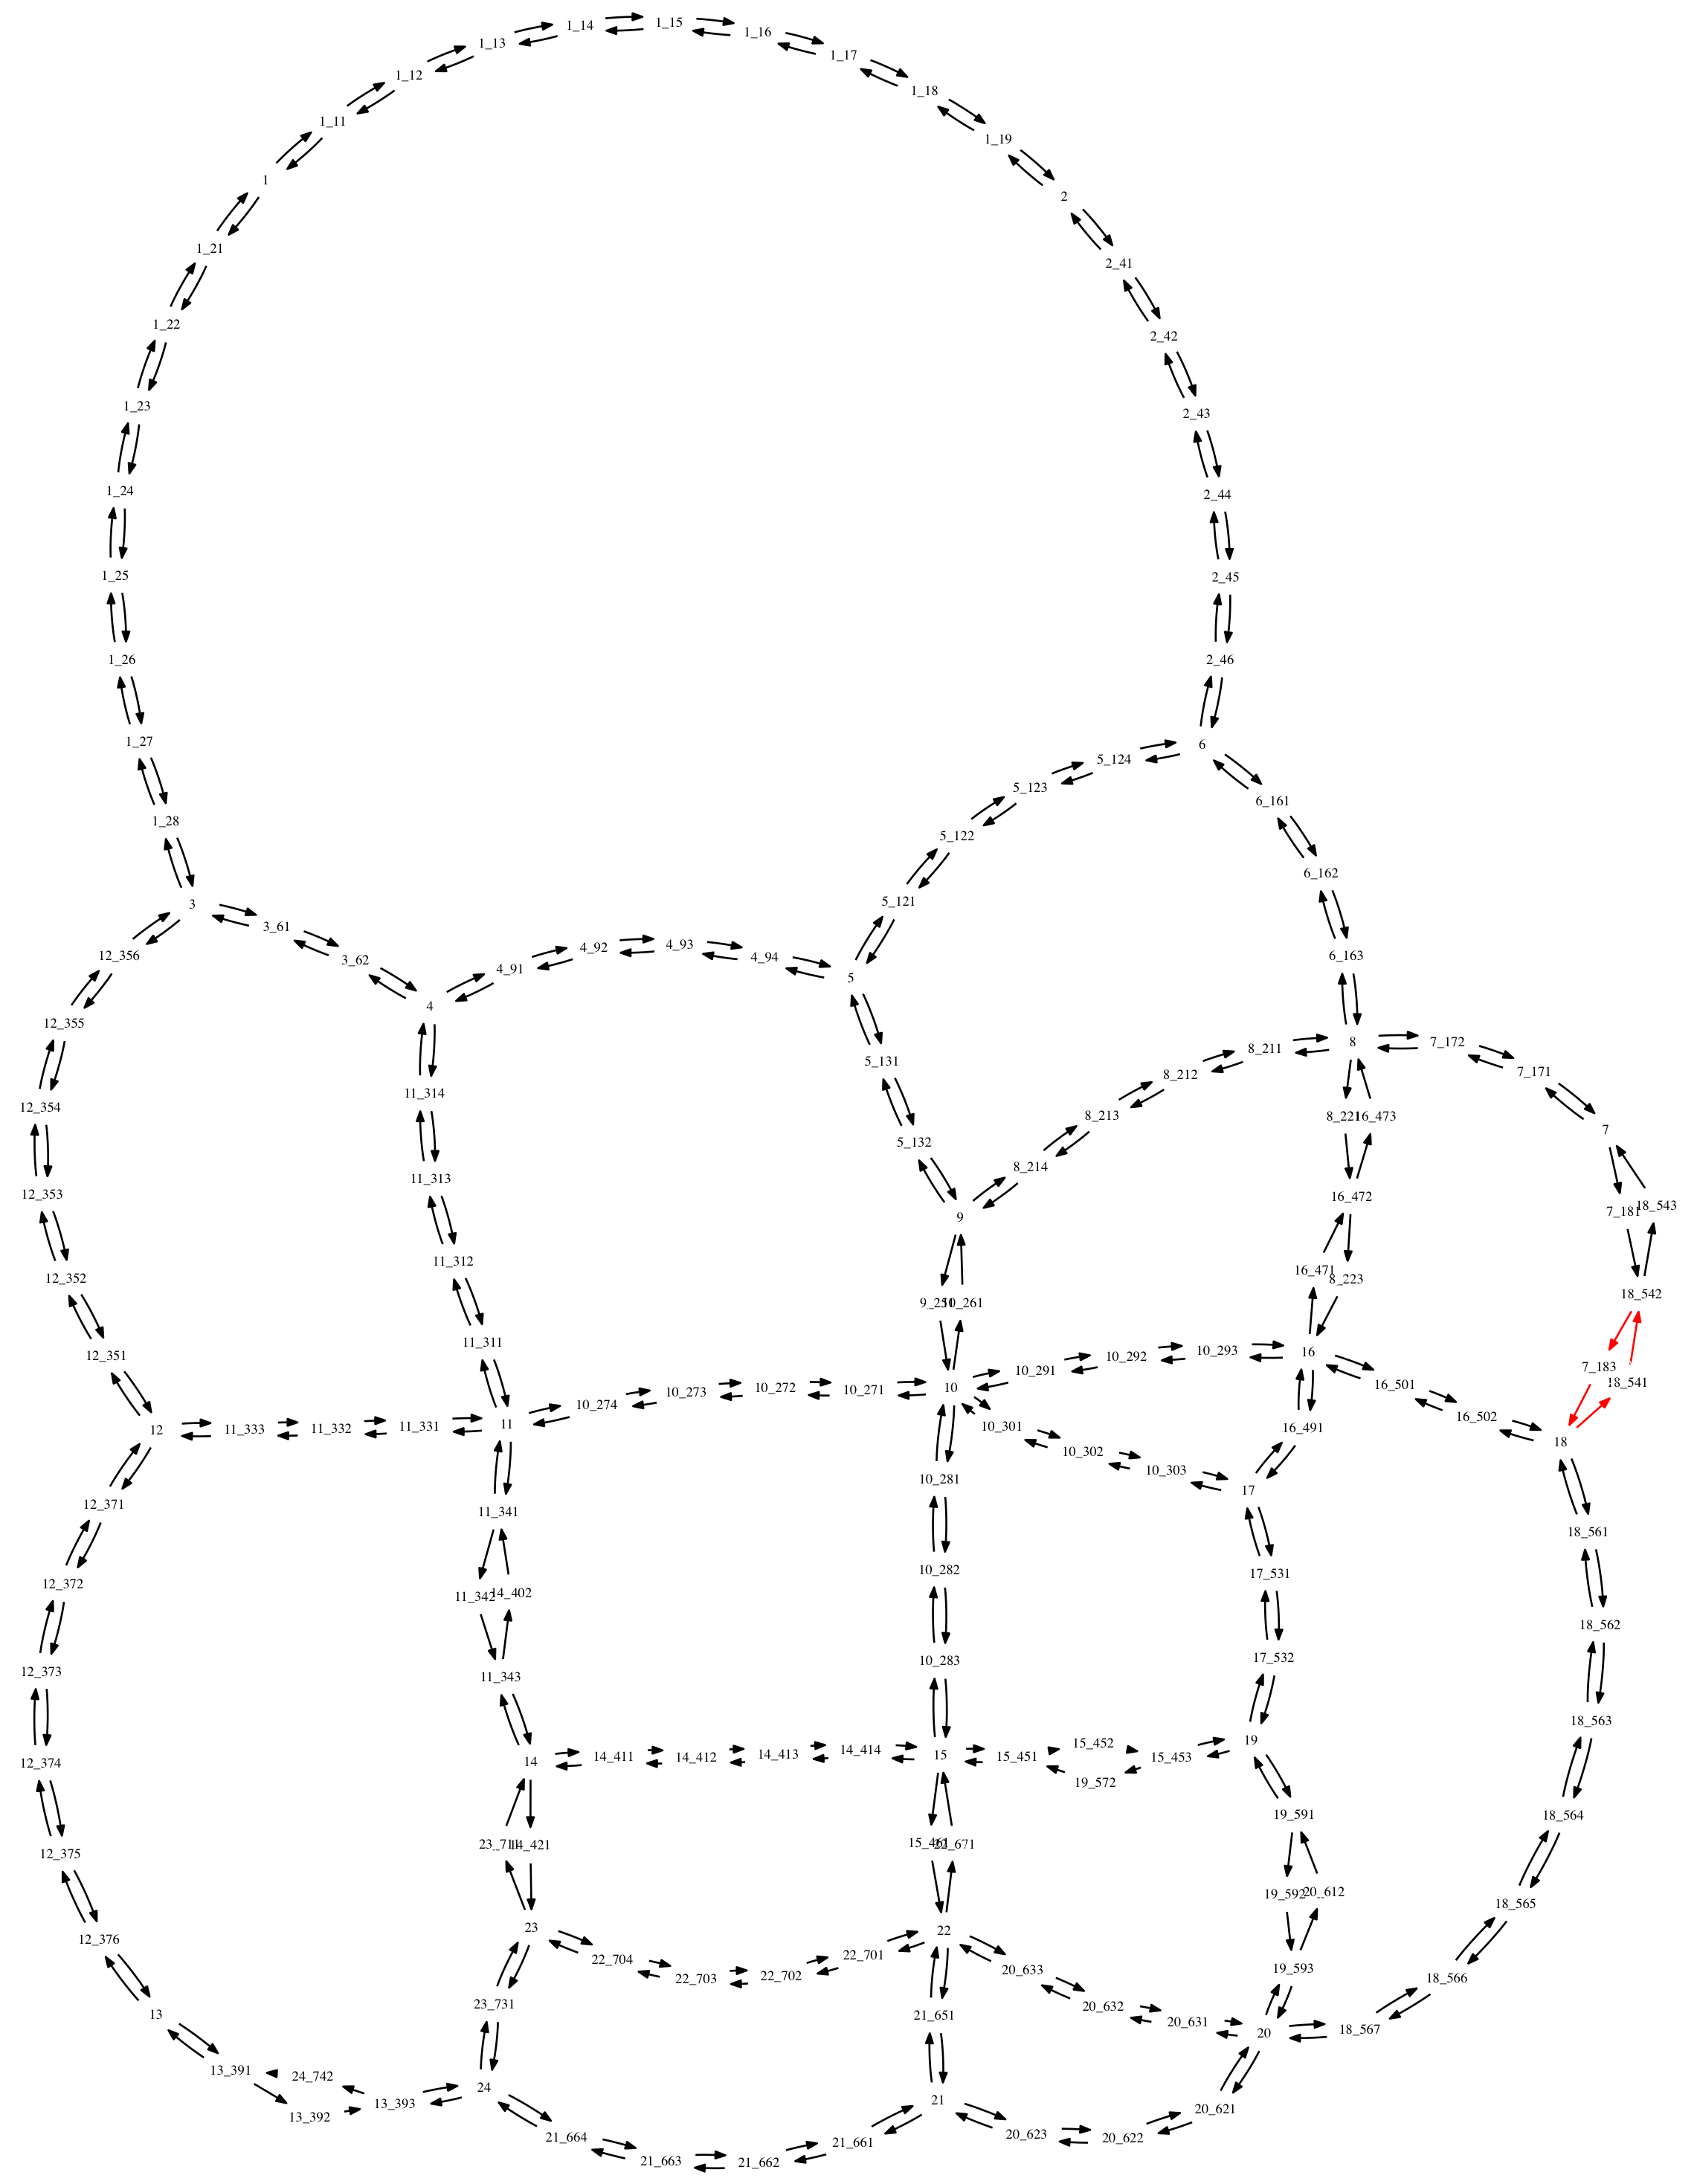
\includegraphics[totalheight=0.550\textheight, angle=90]{img/sioux-out/network1}};
	
	\draw[red,ultra thick] (7.7,9.5) rectangle (9.5,0 |- image.north);
	\fill [draw=none, fill=white, fill opacity=0.8] 
		(image.south west) 			rectangle (7.7	,0 |- image.north)
		(7.7	,0 |- image.south) 	rectangle (9.5	,9.5)
		(9.5	,0 |- image.south) 	rectangle (image.north east);
\end{tikzpicture}
\caption{Fragment grafu z zaznaczonym wspólnym obszarem pierwszym}
\label{fig:frag_1}
\end{figure}

Ciekawym jest jednak obszar wspólny dla wyników prezentowanych na rysunkach~\ref{fig:sioux5}, \ref{fig:sioux7}, \ref{fig:sioux9}, \ref{fig:sioux10}, \ref{fig:sioux11}, \ref{fig:sioux12}, \ref{fig:sioux13}, \ref{fig:sioux14}, \ref{fig:sioux16} Jest to obszar znajdujący się pomiędzy wierzchołkami $15$ i~$19$. Analizując położenie tych ulic w~mieście, obszar ten znajduje się niedaleko bardzo zakorkowanych ulic, często używanych przez agentów symulacji. Region ten można określić jako centrum miasta. Na pewno wielu agentów dociera tam w~ramach pracy lub swoich zainteresowań.~Jego usunięcie może znacząco wpływać na wybór drogi, jak również na sposób dojazdu do miejsc znajdujących się w~okolicy. Oczywiście, pomimo że w~symulatorze węzły te nie były dostępne dla aut, agenci dalej mogli docierać do swoich celów, zostawiając auto w~uprzednio wybranym punkcie. Opisywany fragment został przedstawiony na rysunku \ref{fig:frag_2}

\begin{figure}[htbp]
\centering
\begin{tikzpicture}
    \node[anchor=south west] (image) at (0,0)
    {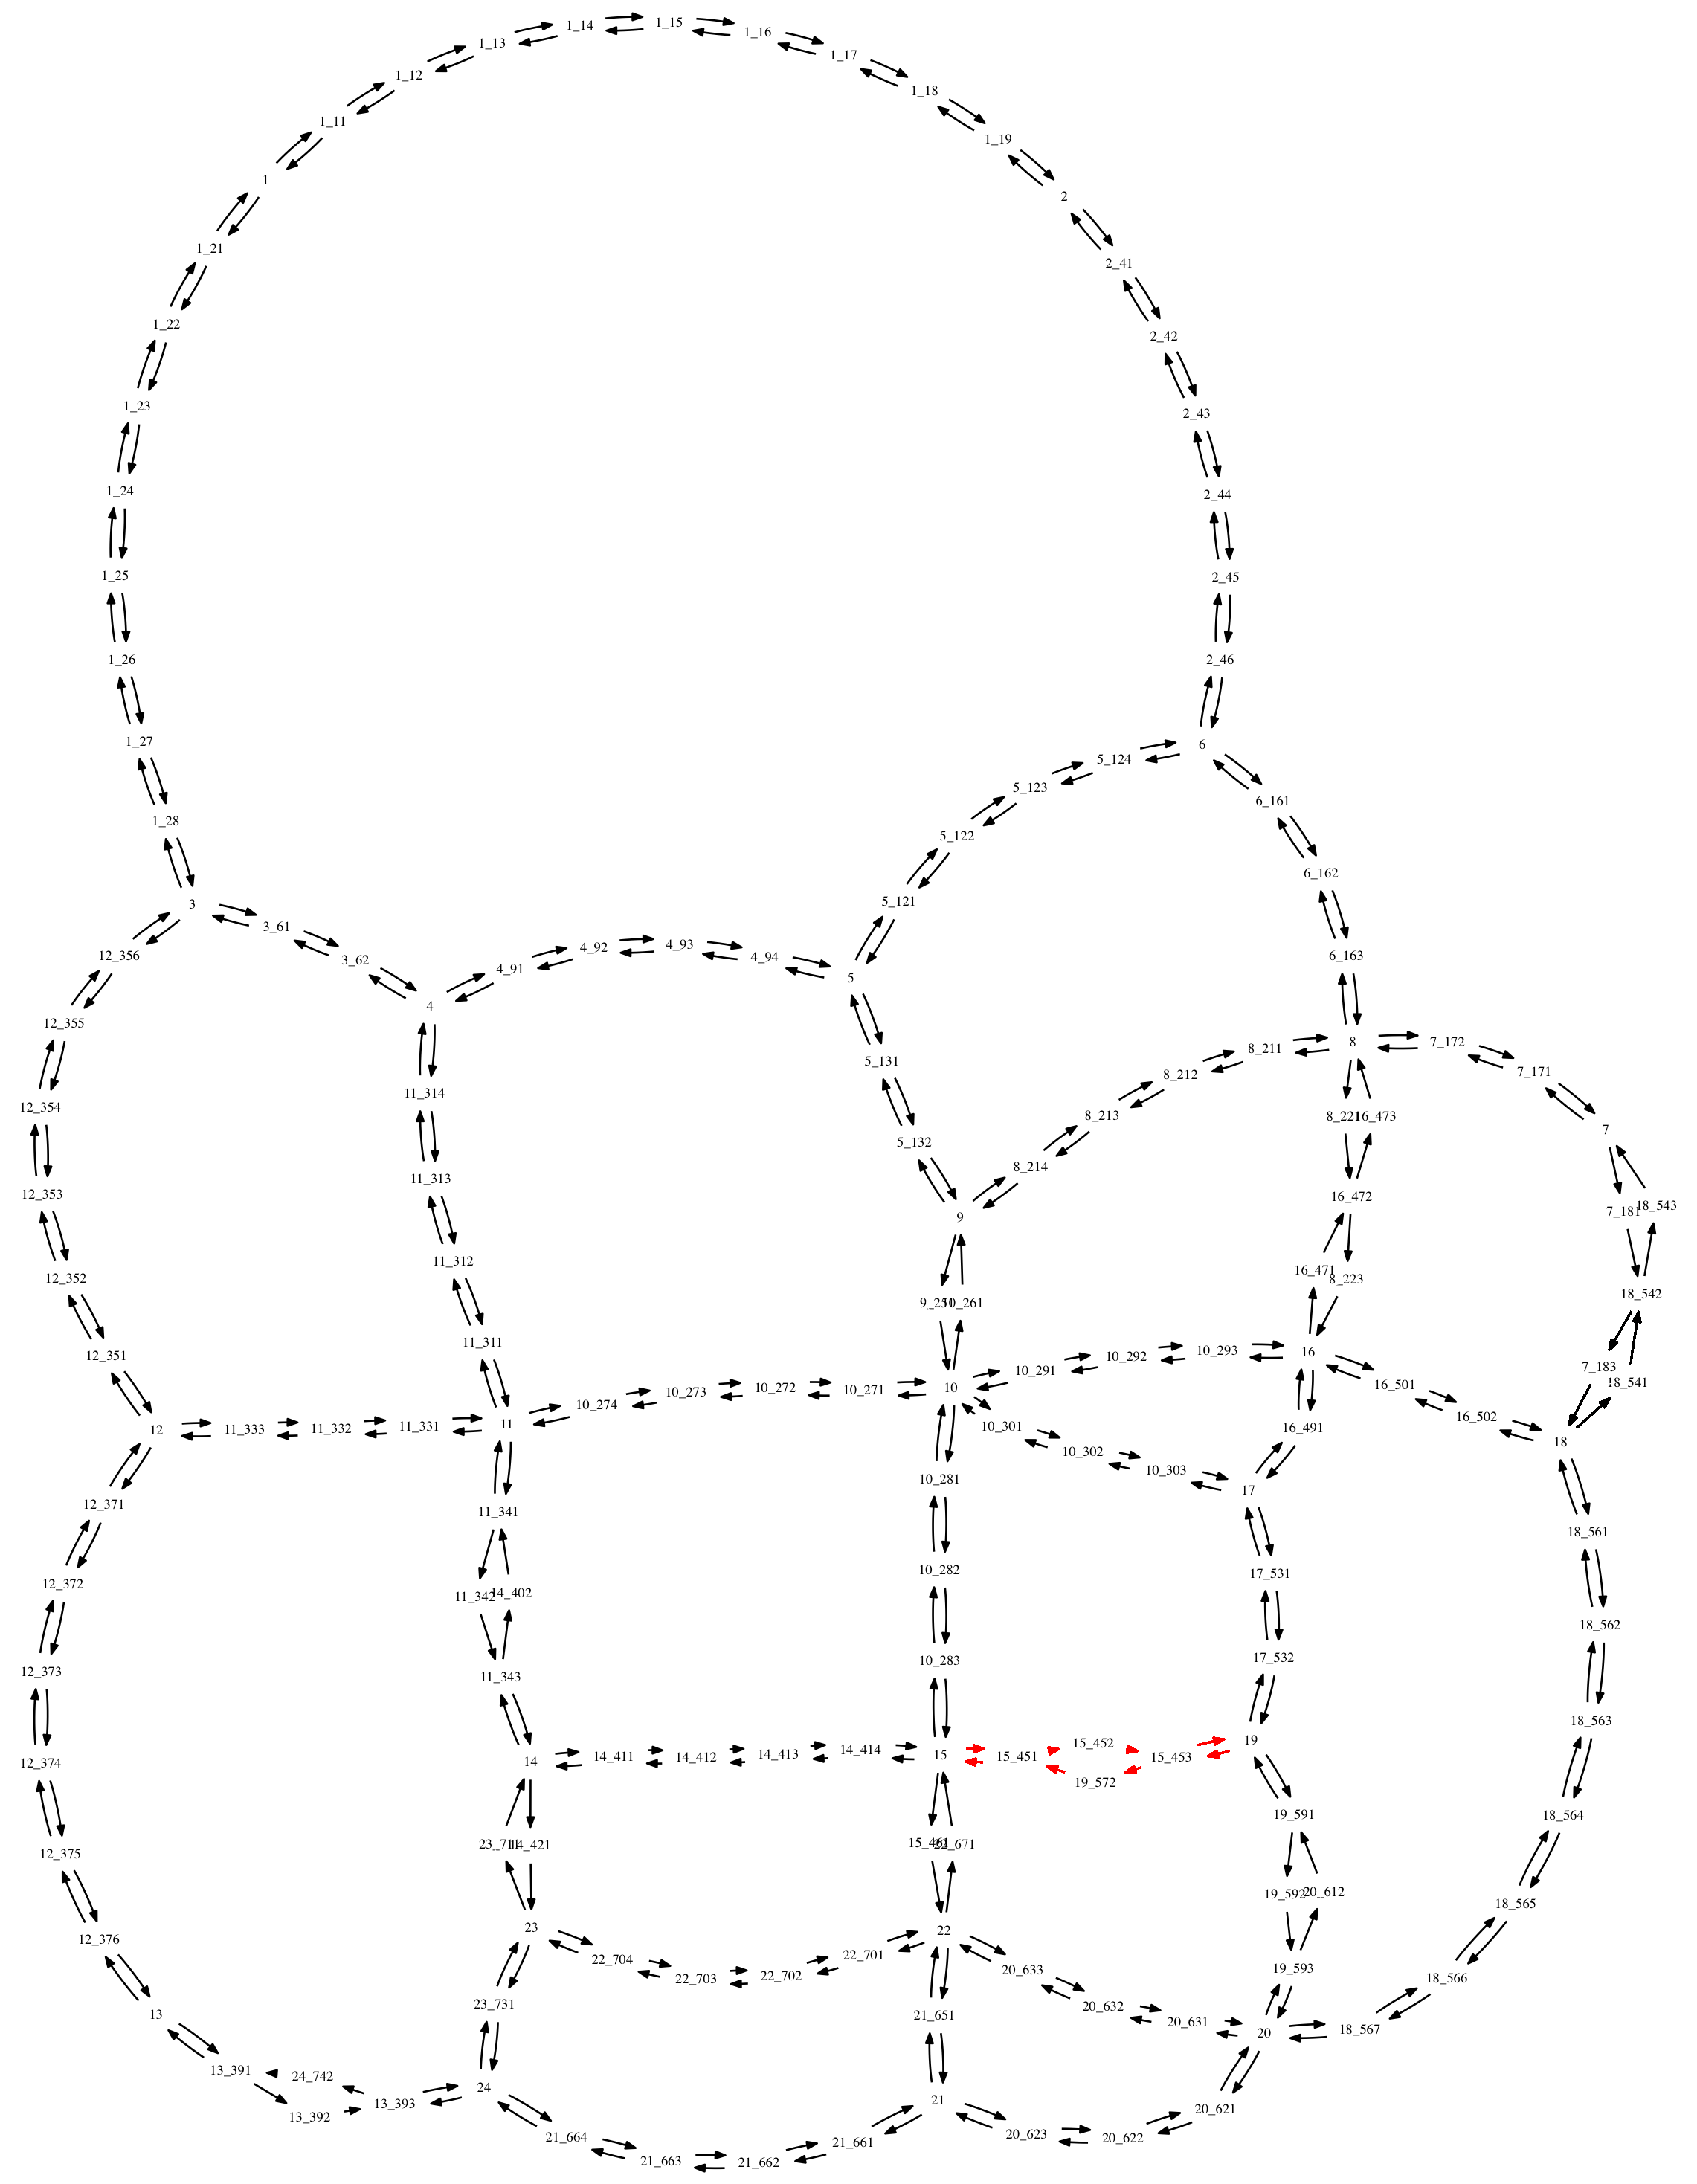
\includegraphics[totalheight=0.550\textheight, angle=90]{img/sioux-out/network2}};
	
	\draw[red,ultra thick] (10.4,5.5) rectangle (11.8,8.3);
	\fill [draw=none, fill=white, fill opacity=0.8] 
		(image.south west) 			rectangle (10.4		,0 |- image.north)
		(10.4	,0 |- image.south) 	rectangle (11.8		,5.5)
		(10.4	,8.3) 				rectangle (11.8		,0 |- image.north)
		(11.8	,0 |- image.south) 	rectangle (image.north east);
\end{tikzpicture}
\caption{Fragment grafu z zaznaczonym wspólnym obszarem drugim}
\label{fig:frag_2}
\end{figure}

Drugim obszarem, który został wybrany w~przypadku paru rozwiązań, są ulice pomiędzy skrzyżowaniem (wierzchołkiem) $5$ i~$6$. Został on wybrany przez rozwiązania prezentowane na rysunkach:~\ref{fig:sioux2}, \ref{fig:sioux4}, \ref{fig:sioux6}, \ref{fig:sioux8}, \ref{fig:sioux12} Region ten jest jednak oddalony od centrum i~prawdopodobnym jest, że zamknięcie drogi wpłynęłoby przede wszystkim negatywnie na dojazd dla wielu osób. Jest to sytuacja analogiczna do tej z~analizowanego wcześniej przypadku przedstawionego na rysunku \ref{fig:frag_1}. Omawiany fragment prezentowany jest na rysunku \ref{fig:frag_3}

\begin{figure}[htbp]
\centering
\begin{tikzpicture}
    \node[anchor=south west] (image) at (0,0)
    {\includegraphics[totalheight=0.550\textheight, angle=90]{img/sioux-out/network3}};
	
	\draw[red,ultra thick] (4.35,5.15) rectangle (6.75,8.0);
	\fill [draw=none, fill=white, fill opacity=0.8] 
		(image.south west) 			rectangle (4.35,0 |- image.north)
		(4.35	,0 |- image.south) 	rectangle (6.75,5.15)
		(4.35	,8.0) 				rectangle (6.75,0 |- image.north)
		(6.75	,0 |- image.south)	rectangle (image.north east);
\end{tikzpicture}
\caption{Fragment grafu z zaznaczonym wspólnym obszarem trzecim}
\label{fig:frag_3}
\end{figure}

Ostatni obszar, który charakteryzował się wspólnym wynikiem dla więcej niż jednego rozwiązania, to jest dla wyników prezentowanych na rysunkach:~\ref{fig:sioux3}, \ref{fig:sioux8}, \ref{fig:sioux15} znajduje się pomiędzy wierzchołkiem $3$ i~$12$. Zaznaczony fragment przedstawiono na rysunku \ref{fig:frag_4}, obróconym o~$90^{\circ}$ w~lewo. Wyraźnie jednak region ten nie znajduje się ani na drodze wielu agentów, ani nie jest węzłem często użytkowanym przez agentów. Jego zamknięcie wpłynęło prawdopodobnie na brak gorszej drogi alternatywnej, którą ten węzeł reprezentował w~wielu przypadkach.

\begin{figure}[htbp]
\centering
\begin{tikzpicture}
    \node[anchor=south west] (image) at (0,0)
    {\includegraphics[totalheight=0.550\textheight, angle=90]{img/sioux-out/network4}};
	
	\draw[red,ultra thick] (5.3,0) rectangle (9.6,1.6);
	\fill [draw=none, fill=white, fill opacity=0.8] 
		(image.south west) 		rectangle (5.3,0 |- image.north)
		(5.3,1.6) 				rectangle (9.6,0 |- image.north)
		(9.6,0 |- image.south) 	rectangle (image.north east);
\end{tikzpicture}
\caption{Fragment grafu z zaznaczonym wspólnym obszarem czwartym}
\label{fig:frag_4}
\end{figure}

Powyższe sugestie mogą zostać użyte w~przypadku poszerzonych badań nad danymi obszarami. Decydując, czy faktycznie mają one wpływ na komunikację w~mieście trzeba przede wszystkim sprawdzić dokładnie drogi wybierane przez agentów scenariusza. W~prezentowanych na rysunkach~\ref{fig:frag_1} --- \ref{fig:frag_4} sieciach drogowych zamknięte drogi zwykle nie znajdowały się w~kluczowych punktach komunikacyjnych, co przede wszystkim wymusza dogłębniejsze zbadanie algorytmu samej symulacji. Otrzymane wyniki nie oznaczają również, że nie istnieje bardziej optymalne rozwiązanie. Przestrzeń przeszukiwań dla powyższego grafu wynosiła $2^{90}$, a~więc zbadanie wszystkich możliwych rozwiązań problemu jest praktycznie niewykonalne.

\section{Analiza zastosowanych ustawień symulacji}
Zgodnie z~wcześniejszymi założeniami, podczas poszukiwań bardziej optymalnej sieci drogowej wybrano ustawienie $10$ iteracji symulacji do oceny sieci. W~celu zweryfikowania wyników, dla najlepszych $17$ sieci przeprowadzono ponowną symulację dla $100$ iteracji. Wyniki te porównano z~wynikami sieci wejściowej. Rysunki~\ref{fig:iters1} --- \ref{fig:iters5} przedstawiają wyniki tych porównań.~Dla poprawienia czytelności wykresy zostały podzielone, prezentując za każdym razem tylko część sieci drogowych. \textbf{Legenda wykresów odnosi się do wyniku uzyskanego przez rozwiązanie, które jest przedstawiane w~tabeli \ref{tab:tabela_wynikow} Numer wyniku sieci odnosi się do numeru identyfikacyjnego sieci.} \textbf{Wyjątek stanowi numer sieci $0$, który odnosi się do sieci wejściowej}, czyli sieci z~dostępnymi wszystkimi ulicami. Rysunek \ref{fig:iters5} przedstawia porównanie najlepszego rozwiązania uzyskanego podczas badań, z~najgorszym oraz z~siecią wejściową.

\begin{figure}[htbp]
\centering
\includegraphics[width=1\textwidth]{img/iters/iters1}
\caption{Wykres zmiany średniego czasu przejazdu od iteracji dla sieci wynikowych o ID 1, 2, 3, 4 z ujęciem sieci wejściowej - 0}
\label{fig:iters1}
\end{figure}

Najbardziej interesującymi punktami na rysunku~\ref{fig:iters1} jest sytuacja podczas pierwszych dwudziestu iteracji i~ta zachodząca w~końcowych iteracjach, osiemdziesiątej i~kolejnych. Przede wszystkim zauważalna jest wyraźna przewaga sieci z~zamkniętymi węzłami, występująca w~początkowych iteracjach, która stopniowo maleje. Ważnym jest również, że podczas gdy wynik uzyskiwany w~kolejnych iteracjach dla sieci wejściowej stopniowo poprawia się, zmiana ta nie jest tak widoczna w~przypadku sieci uzyskanych podczas badań. W~iteracji setnej, ostatniej sieć z~numerem 4 (Rys. \ref{fig:sioux4}) uzyskuje gorszy wynik niż sieć wejściowa, natomiast wyniki pozostałych sieci (Rys. \ref{fig:sioux1} --- \ref{fig:sioux3}) są marginalnie lepsze.

\begin{figure}[htbp]
\centering
\includegraphics[width=1\textwidth]{img/iters/iters2}
\caption{Wykres zmiany średniego czasu przejazdu od iteracji dla sieci wynikowych  o ID 5, 6, 7, 8 z ujęciem sieci wejściowej - 0}
\label{fig:iters2}
\end{figure}

Nie jest zaskoczeniem, że w~przypadku danych, pokazanych na rysunku~\ref{fig:iters2} sytuacja powtarza się. Początkowo duża przewaga sieci uzyskanych podczas badań zaciera się. Iteracje ponownie nieznacznie wpływają na polepszanie się wyników uzyskanych przez rozwiązania o~identyfikatorach: 5, 6, 7, 8 (Rys. \ref{fig:sioux5} --- \ref{fig:sioux8}). Wszystkie sieci oprócz sieci o~identyfikatorze 6 (Rys. \ref{fig:sioux6}) w~setnej iteracji okazują się jednak lepsze od sieci wejściowej, posiadającej wszystkie dostępne ulice (węzły). Wartym zauważenia jest, że w~przypadku dłuższej symulacji kolejność rozwiązań byłaby inna niż obecnie.

\begin{figure}[htbp]
\centering
\includegraphics[width=1\textwidth]{img/iters/iters3}
\caption{Wykres zmiany średniego czasu przejazdu od iteracji dla sieci wynikowych  o ID 9, 10, 11, 12 z ujęciem sieci wejściowej - 0}
\label{fig:iters3}
\end{figure}

W przypadku rozwiązań o~identyfikatorach: 9, 10, 11, 12 (Rys.~\ref{fig:sioux9} --- \ref{fig:sioux12}) wyniki nie są już jednak tak obiecujące. Trend poprzednich wykresów utrzymuje się i~w~przypadku wykresu na rysunku \ref{fig:iters3} wyraźnie widać, że sieć wejściowa w~setnej iteracji uzyskuje lepszy wynik niż uzyskane rozwiązania. Sytuacja jest jeszcze bardziej widoczna dla kolejnych rozwiązań: 13, 14, 15, 16 i~17 (Rys. \ref{fig:sioux13} --- \ref{fig:sioux17}), których wyniki jeszcze bardziej różnią od tych uzyskanych przez sieć wejściową (Rys. \ref{fig:iters4}). Wybór wyższego parametru iteracji symulacji MATSim, omawianej w~podrozdziale \ref{rozdz.ustawienia_symulatora}, wpłynąłby zatem znacznie  na liczbę otrzymanych sieci wynikowych, zmniejszając tę pulę o~połowę.

\begin{figure}[htbp]
\centering
\includegraphics[width=1\textwidth]{img/iters/iters4}
\caption{Wykres zmiany średniego czasu przejazdu od iteracji dla sieci wynikowych o ID 13, 14, 15, 16, 17 z ujęciem sieci wejściowej - 0}
\label{fig:iters4}
\end{figure}

\begin{figure}[htbp]
\centering
\includegraphics[width=1\textwidth]{img/iters/iters5}
\caption{Wykres zmiany średniego czasu przejazdu od iteracji dla sieci najlepszej i najgorszej (1, 17) z ujęciem sieci wejściowej - 0}
\label{fig:iters5}
\end{figure}

Wykresy prezentowane  na rysunkach~\ref{fig:iters1} --- \ref{fig:iters4} doskonale podsumowuje wykres na rysunku \ref{fig:iters5}, gdzie najlepsze rozwiązanie porównywane jest z~najgorszym. Sieć wejściowa oraz zmiana wyniku pozwala wyciągnąć wnioski na temat działania samego symulatora.

Symulator \textit{MATSim} zadziałał zgodnie z~oczekiwaniami, wykazując dużą zdolność adaptacji agentów do sieci. Przypadek ten można opisać, zadając sobie pytanie, skąd właściwie biorą się ,,korki'' i~zatory drogowe? Są one zwykle efektem braku poprawnego planu podróży uczestników ruchu. Symulator potrafi znaleźć taki plan, który w~sposób idealny dobiera czas podróży oraz najlepszą drogę. Jest to oczywiście możliwe dzięki powtarzającym się w~każdej iteracji \textbf{tym samym} warunkom drogowym, które panują w~sieci. Scenariusz symulacji transportu ruchu drogowego jest bowiem pozbawiony losowych wypadków oraz czynników ludzkich. Nie jest to więc sytuacja rzeczywista.

Mając na uwadze ten ,,idealny'' aspekt symulacji, wybory w~iteracjach wcześniejszych są mniej idealne, można powiedzieć, bardziej ludzkie. Wykresy zaprezentowane na rysunkach~\ref{fig:iters1} --- \ref{fig:iters5} wyraźnie pokazują, że dla zmodyfikowanej sieci, znacznie trudniej jest popełnić błąd przy planowaniu trasy, mając ograniczoną wiedzę na temat warunków drogowych. Wymuszenie określonych dróg na agentach pozwoliło im szybciej dokonywać prawidłowych wyborów.

W przypadku długiej symulacji, część sieci zmodyfikowanych osiągała gorszy rezultat niż sieć wejściowa. Oprócz wyżej wymienionych czynników, trzeba bowiem pamiętać, że generalnie większa liczba węzłów oznacza większe możliwości przepływowe sieci. Efekt dłuższej symulacji można porównać z~dopasowaniem sieci drogowej do potrzeb zadanego modelu agentów. Taka sieć spełniałaby idealnie wymogi danej symulacji. Nie sprawdziłaby się jednak, gdyby model został zmieniony. W~przypadku długiej nauki agentów, na temat danej sieci, zachodzi sytuacja odwrotna. Ich wiedza nie musiałaby sprawdzić się w~przypadku zmiany ich planów dnia lub wystąpienia losowych czynników na drodze.

W powyższym rozdziale przedstawiono wyniki potwierdzające możliwość optymalizacji sieci drogowej przy użyciu algorytmów genetycznych i~paradoksu Braessa. Wyniki zawierają opis oraz omówiono konsekwencje użytych parametrów symulacji. Kolejny rozdział zawiera podsumowanie pracy oraz możliwości jej rozwoju.

\chapter{Podsumowanie}\label{rozdz.podsumowanie} 
Uzyskane wyniki w~ramach poniższej pracy dyplomowej potwierdzają możliwość zoptymalizowania sieci drogowej poprzez zamknięcie określonych ulic, przy użyciu algorytmu genetycznego. Dla zadanej sieci drogowej, poprzez optymalizację, uzyskano kilkanaście rozwiązań, które mogą posłużyć jako baza do dalszych badań.~Zastosowana metoda oceny rozwiązań, czyli zewnętrzny symulator ruchu drogowego również spełnił oczekiwania projektowe. Trzeba jednak pamiętać, że uzyskane wyniki są czysto teoretyczne, a~całość eksperymentu została przeprowadzona przy wielu uproszczeniach.

Pierwszym uproszczeniem jest oczywiście sam symulator. Po pierwsze, w~założeniu został zbadany tylko jeden model populacji oraz aktywności dnia (agentów). Model ten przedstawia pewne uśrednienie demograficzne mieszkańców miasta Sioux Falls oraz ich planów komunikacyjnych. Po drugie, w~badanym wariancie miasto zostało pozbawione komunikacji miejskiej, co miało na celu zintensyfikowanie ruchu transportu prywatnego. Po trzecie, symulator w~sposób nierzeczywisty dokonuje optymalizacji planów dnia agentów, które mogą zostać uznane za nierzeczywiste. Trudnym jest jednak oszacowanie stopnia ,,sztuczności'' dopasowania planu do spodziewanych warunków drogowych.

Drugim uproszczeniem jest model miasta. Z~założenia stosowana jest sieć z~pominięciem pomniejszych dróg, mało istotnych dla ogółu komunikacji w~mieście. Kontynuując, model zakłada jedynie ruch, który jest generowany przez mieszkańców, z~pominięciem ruchu napływającego z~innych rejonów. Ostatnim są sytuacje losowe, spowodowane zwykle przez czynnik ludzki. Model nie przewiduje awarii, remontów, wypadków, które oczywiście są składnikiem codziennych sytuacji w~mieście. 

Podczas badań możliwe jest zastosowanie innego kryterium oceny rozwiązań.~Zmiana symulatora lub zupełnie inna metoda oceny tworzonych sieci wpłynie bezsprzecznie na otrzymane wyniki.

Pamiętając zatem, że prezentowane rozwiązanie miało  dostarczyć pewnej sugestii w~sprawie usprawnienia ruchu, spełnia ono swoje zadanie. Innowacja nawet tak dobrze rozwiniętych miast, jak te w~USA jest możliwa, niekoniecznie poprzez kosztowne inwestycje w~tworzenie nowej infrastruktury. 

\section{Perspektywy dalszych badań w~dziedzinie}
Dość oczywistym kierunkiem rozwoju może być oczywiście dalsze przeszukiwanie opisanego problemu. Jak już zostało wspomniane wyżej, ilość możliwych rozwiązań jest bardzo duża ($2^{90}$). Jak zostało przedstawione, zmiana parametrów samej symulacji, również wpłynie na otrzymywane wyniki.

Ciekawszym wydaje się być jednak przeszukiwanie nowych zbiorów. W~przypadku symulatora \textit{MATSim} istnieje pokaźna liczba przykładów opartych o~rzeczywiste miasta, na których były prowadzone symulacje. Jeden z~dostępnych modeli jest odwzorowaniem miasta Berlin (Rys.~\ref{fig:berlin}), przy okazji, wykonanym z~dużo większą dokładnością niż Sioux Falls.

\begin{figure}[htbp]
\centering
\includegraphics[width=0.82\textwidth]{img/berlin2}
\caption{Sieć drogowa miasta Berlin w postaci grafu}
\label{fig:berlin}
\end{figure}

Ponadto, w~pracy można wykorzystać inne twierdzenia i~paradoksy dotyczące m.in. transportu miejskiego. Niestety, jak już było wspomniane wcześniej, wiele z~tych praw jest opartych o~psychologiczne tezy, bez matematycznego podparcia, co powoduje, że wyniki są trudne do przewidzenia.

\cleardoublepage
\phantomsection
\addcontentsline{toc}{chapter}{\listfigurename} 
\listoffigures

\cleardoublepage
\phantomsection
\addcontentsline{toc}{chapter}{\listtablename} 
\listoftables

\cleardoublepage
\phantomsection
\addcontentsline{toc}{chapter}{\lstlistlistingname}
\lstlistoflistings

\cleardoublepage
\phantomsection
\addcontentsline{toc}{chapter}{\bibname} 
\begin{thebibliography}{99}

\bibitem{genetyczne}
	D.~Rutkowska, M.~Piliński i~L.~Rutkowski,
	\textit{Sieci neuronowe, algorytmy genetyczne i~systemy rozmyte},
	PWN, Warszawa 1997.
	
\bibitem{genetyczne-dane=ewo}
	Michalewicz Z., 
	\textit{Algorytmy genetyczne + struktury danych = programy ewolucyjne}, 
	Wydawnictwo Naukowo-Techniczne, Warszawa 1999.
	
\bibitem{genetyczne-immunologiczne}
	S.~T.~Wierzchoń, 
	\textit{Sztuczne systemy immunologiczne. Teoria i~zastosowania},
	Akademicka Oficyna Wydawnicza EXIT, Warszawa 2001

\bibitem{gene}
	Mitchell Melanie,
	\textit{An Introduction to Genetic Algorithms},
	A~Bradford Book The MIT Press, 1998.	
	
\bibitem{investigation} 
	Leslie Arthur Keith Bloy, 
	\textit{An investigation into Braess’ paradox}, 
	Thesis, 02/2007.

\bibitem{paradox}
	Dietrich Braess,
	\textit{Über ein Paradoxon aus der Verkehrsplanung. ,,Unternehmensforschung''},
	1968 (niem.).
	
\bibitem{paradox-eng}
	A.~Nagurney, and T.~Wakolbinger,
	\textit{On a~Paradox of Traffic Planning, translated from the (1968) original D.~Braess paper from German to English by D.~Braess},
	Transportation Science 39/4, 2005.

\bibitem{newinsights}
	Rric Pas and Shari Principio,
	\textit{Braess’ paradox: Some new insights}, 
	April 1996.
	
\bibitem{paradox-dowod}
	Richard Steinberg and Willard I.~Zangwill,
	\textit{The Prevalence of Braess' Paradox},
	Transportation Science Vol.~17, No. 3, August 1983. 

\bibitem{grafy}
	Łukasz Kowalik,
	\textit{Algorytmy i~struktury danych, grafy},
	Wykład, 2003.
	
\bibitem{teoria-grafow}
	Robin J.~Wilson,
	\textit{Introduction to Graph Theory},
	5th edition, Pearson, 2010.
	
\bibitem{teoria-grafow-z-zast}
	J.~A.~Bondy and U. S.~R.~Murty,
	\textit{Graph theory with applications},
	North Holland, 5th printing, 1982.
	
\bibitem{siux}
	A.~Chakirov,
	\textit{Enriched Sioux Falls Scenario with Dynamic Demand},
	MATSim User Meeting, Zurich/Singapore, June 2013.
		
\bibitem{matsim-userg}
	M.~Rieser, C.~Dobler, T.~Dubernet, D.~Grether, A.~Horni, G.~Lammel, R.~Waraich, M.~Zilske, Kay W.~Axhausen, Kai Nagel,
	\textit{MATSim User Guide},
	updated October 30, 2014.

\bibitem{reducingtheeffects}
	Ana L.~C.~Bazzan and Franziska Klügl,
	\textit{Reducing the Effects of the Braess Paradox with Information Manipulation}.

\bibitem{conference} 
	Wataru Nanya, Hiroshi Kitada, Azusa Hara, Yukiko Wakita, Tatsuhiro Tamaki, and Eisuke Kita,
	\textit{Road Network Optimization for Increasing Traffic Flow},
	Int. Conference on Simulation Technology, JSST 2013.

\bibitem{tarjan}
	Tarjan, R. E.,
	\textit{Depth-first search and linear graph algorithms},
	SIAM Journal on Computing, Vol 1, No. 2, 06.1972
	
\bibitem{braess}
	Polskie tłumaczenie paradoksu Braessa,
	\url{http://pl.wikipedia.org/wiki/Paradoks_Braessa},
	dostęp 10.04.2015.
	
\bibitem{urban}
	Marek Karabon, Kontr-intuicyjne metody ograniczania korków w~miastach,
	\url{http://www.tnn.pl/k_675_m_3.html},
	dostęp 10.04.2015.
	
\bibitem{lewis}
	Wojciech Szymalski: Prawo Lewisa-Mogridge’a w~Warszawie – wprowadzenie,
	\url{http://www.zm.org.pl/?a=lewis-mogridge-14-00_wprowadzenie},
	dostęp 10.04.2015.
	   
\bibitem{silniespojny}
	Matematyczne twierdzenie grafu silnie spójnego,
	\url{http://mathworld.wolfram.com/StronglyConnectedDigraph.html},
	dostęp 10.04.2015.	

\bibitem{matsim}
	Strona główna projektu MATSim,
	\url{http://matsim.org},
	dostęp 10.04.2015.

\bibitem{math}
	Strona główna projektu Apache Commons Math,
	\url{http://commons.apache.org/proper/commons math},
	dostęp 10.04.2015.
	
\bibitem{networkx}
	Strona główna projektu NetworkX,
	\url{http://networkx.github.io},
	dostęp 10.04.2015.
	
\bibitem{ubuntu}
	Strona główna systemu Linux Ubuntu,
	\url{http://www.ubuntu.com},
	dostęp 10.04.2015.
	
\bibitem{azure}
	Strona główna chmury Microsoft Azure,
	\url{http://azure.microsoft.com},
	dostęp 10.04.2015.
		
\bibitem{elektrony}
	Max Planck Institute, 
	\textit{Study: Solar and wind energy may stabilize the power grid},
	R\&D Magazine, 14.09.2012	

\bibitem{nanoskopia}
	M.~Pala, S.~Baltazar, P.~Liu, H.~Sellier, B.~Hackens, F.~Martins, V.~Bayot, X.~Wallart, L.~Desplanque, S.~Huant,
	\textit{Transport Inefficiency in Branched-Out Mesoscopic Networks: An Analog of the Braess Paradox},
	Physical Review Letters 108, 06.12.2011.

\end{thebibliography}

\clearpage
\phantomsection
\addcontentsline{toc}{chapter}{Abstract}
\chapter*{Abstract}

The purpose of the present master thesis was to find an optimal solution of the given road network using genetic algorithm. The optimisation is performed using fixed set in advance parameters. This thesis covers two main fields of presented subject. Firstly it introduces the topic of road network optimisation and Braess paradox. Secondly, it describes the techniques used to achieve the final goal.

The application performing the optimisation process uses an external ranking system. In the case described in the thesis, a~multiagent simulator, MATsim. The aspects of the simulation concering the final results of the project are also described. 

The solution is prepared using Java and Python programming languages. During the research, the process was conducted by a~machine operating on Linux Ubuntu 12.04 LTS.

The final result proves the validity of the introduced methods: the genetic algorithm, regarding searching of the optimal solution, as well as the simlation based rank using the multiagent  simulator resulted in several solutions of the given network with given parameters.

The discussion regarding the \textit{MATSim's} iteration results and configuration also explain the differences in long-term evaluation of the simulation. Since the optimal parameters for any simulation are discussable, in the thesis the main goal was to find a~simple, fast solution to experienced problem. Therefore, lower average time of travel for agents during longer iterations would be a~separate case of study.

\clearpage
\thispagestyle{empty}
\mbox{}
\includepdf[pages=-]{doc/Zalacznik1.pdf}

\clearpage
\includepdf[pages=-]{doc/Zalacznik2.pdf}

\end{document}
